% \documentclass[landscape,final]{baposter}
\documentclass[a0poster,portrait,final,movebody=-5pt]{baposter}
% \documentclass[a4shrink,portrait,final]{baposter}
% Use a4shrink for an a4 sized paper.

%\tracingstats=2

\usepackage[english]{babel}
\usepackage{times}
\usepackage{calc}
\usepackage{graphicx}
\usepackage{amsfonts} 
\usepackage{cmbright}
\usepackage{amsmath}
\usepackage{amsthm}
\usepackage{amssymb}
\usepackage{relsize}
\usepackage{multirow}
\usepackage{bm}
\usepackage{lpic}
\usepackage{fontspec}
\setsansfont [ BoldFont={Akkurat Office},  ItalicFont={Akkurat Light Office Italic}, BoldItalicFont={Akkurat Office Italic} ] {Akkurat Light Office}
\setmainfont [ BoldFont={Akkurat Office},  ItalicFont={Akkurat Light Office Italic}, BoldItalicFont={Akkurat Office Italic} ] {Akkurat Light Office}

\newboolean{articletitles}
\setboolean{articletitles}{true}
\newboolean{uprightparticles}
\usepackage{xspace}
\usepackage{fancyvrb}
\usepackage{rccol}
\rcRoundingfalse
\usepackage{tabularx}
\usepackage{siunitx}
\usepackage{upgreek}
\usepackage{paralist}
%\setdefaultleftmargin{0pt}{}{}{}{}{}
%% JpsiKS specific
\def\BdToJPsiKS  {\decay{\Bd}{\jpsi\KS}}
\def\BdToJPsiKstar  {\decay{\Bd}{\jpsi\Kstar}}
\def\BuToJPsiK  {\decay{\Bu}{\jpsi\Kp}}
\def\SJpsiKS     {\ensuremath{S_{\jpsi\KS}}\xspace}
\def\CJpsiKS     {\ensuremath{C_{\jpsi\KS}}\xspace}
\def\Sf     {\ensuremath{S_{f}}\xspace}
\def\Cf     {\ensuremath{C_{f}}\xspace}
\def\sintwobeta   {\ensuremath{\sin 2\beta}\xspace}
\def\etaOS {\eta^{\text{OS}}}
\def\Deltaomega {\Delta p_0}
\def\JPsiTomumu	{\decay{\jpsi}{\mumu}}
\def\KSTopipi	{\decay{\KS}{\pipi}}
\def\BdToDstmunu	{\decay{\Bd}{\Dstarm\mup\neum}}
\def\DsTophiKKpi	{\decay{\Ds}{\phi(\KpKm)\pim}}
\def\DsToKstKpiK	{\decay{\Ds}{\Kstarz(\Kp\pim)\Km}}
\def\DsToKKpi		{\decay{\Ds}{\KpKm\pim}}
\def\DsToKpipi		{\decay{\Ds}{\Km\pipi}}
\def\DsTopipipi		{\decay{\Ds}{\pim\pipi}}

\newcommand{\Bztag}{\ensuremath{\widehat{\B^0}}\xspace}
\newcommand{\Bzbtag}{\ensuremath{\widehat{\Bbar^0}}\xspace}

\newcommand{\pref}[1]{\ref{#1} on page~\pageref{#1}\xspace}

% Convenience functions
\newcommand{\asymbol}[3]{
\ensuremath{#1
^{\ForEach{;}{
\ifboolexpr{test {\ifnumcomp{\the\thislevelcount}{=}{1}}}
  {\text{\thislevelitem}}
  {, \text{\thislevelitem}}
}{#2}}
_{\ForEach{;}{
\ifboolexpr{test {\ifnumcomp{\the\thislevelcount}{=}{1}}}
  {\text{\thislevelitem}}
  {, \text{\thislevelitem}}
}{#3}}
\xspace}
}

\newcommand{\pdf}[2]{\asymbol{\mathcal{P}}{#1}{#2}}
\newcommand{\res}[2]{\asymbol{\mathcal{R}}{#1}{#2}}
\newcommand{\norm}[2]{\asymbol{\mathcal{N}}{#1}{#2}}
\newcommand{\effc}[2]{\asymbol{\epsilon}{#1}{#2}}
\newcommand{\yield}[2]{\asymbol{N}{#1}{#2}}
\newcommand{\parvec}[2]{\asymbol{\lambda}{#1}{#2}}
\newcommand{\param}[3]{\asymbol{#1}{#2}{#3}}

\newcommand{\SPlot}{\ensuremath{_{s}\mathcal{P}lot}\xspace}
\newcommand{\SPlots}{\ensuremath{_{s}\mathcal{P}lots}\xspace}
\newcommand{\SPlotweight}{\ensuremath{_{s}\mathcal{P}_\text{n}}\xspace}

\SaveVerb{Hlt1u}=Hlt1u=
\SaveVerb{Hlt2u}=Hlt2u=
\SaveVerb{Hlt2b}=Hlt2b=


% Definitions to have correct line numbering even when using AMS math's align
% taken from http://phaseportrait.blogspot.de/2007/08/lineno-and-amsmath-compatibility.html

%\newcommand*\patchAmsMathEnvironmentForLineno[1]{%
%  \expandafter\let\csname old#1\expandafter\endcsname\csname #1\endcsname
%  \expandafter\let\csname oldend#1\expandafter\endcsname\csname end#1\endcsname
%  \renewenvironment{#1}%
%     {\linenomath\csname old#1\endcsname}%
%     {\csname oldend#1\endcsname\endlinenomath}}% 
%\newcommand*\patchBothAmsMathEnvironmentsForLineno[1]{%
%  \patchAmsMathEnvironmentForLineno{#1}%
%  \patchAmsMathEnvironmentForLineno{#1*}}%
%\AtBeginDocument{%
%\patchBothAmsMathEnvironmentsForLineno{equation}%
%\patchBothAmsMathEnvironmentsForLineno{align}%
%\patchBothAmsMathEnvironmentsForLineno{flalign}%
%\patchBothAmsMathEnvironmentsForLineno{alignat}%
%\patchBothAmsMathEnvironmentsForLineno{gather}%
%\patchBothAmsMathEnvironmentsForLineno{multline}%
%}
%%% $Id: lhcb-symbols-def.tex 13914 2012-01-20 18:57:29Z jwishahi $
%%% ======================================================================
%%% Purpose: standard LHCb aliases
%%% Author: Originally Ulrik Egede, adapted by Tomasz Skwarnicki for templates,
%%% rewritten by Chris Parkes
%%% Created on: 2009-09-24
%%% =======================================================================

%%% this has to go before \begin{document}
%%%\usepackage{ifthen} 
%%%\newboolean{uprightparticles}
%%%\setboolean{uprightparticles}{true} %Set to false to get italic particle symbols

%%% Add comments with at least three %%% preceding.
%%% Add new sections with one % preceding
%%% Add new subsections with two %% preceding

%%%%%%%%%%%%%
% Experiments
%%%%%%%%%%%%%
\def\lhcb {LHCb\xspace}
\def\ux85 {UX85\xspace}
\def\cern {CERN\xspace}
\def\lhc {LHC\xspace}
\def\atlas {ATLAS\xspace}
\def\cms {CMS\xspace}
\def\babar  {BaBar\xspace}
\def\belle  {Belle\xspace}
\def\aleph  {ALEPH\xspace}
\def\delphi {DELPHI\xspace}
\def\opal   {OPAL\xspace}
\def\lthree {L3\xspace}
\def\lep    {LEP\xspace}
\def\cdf    {CDF\xspace}
\def\dzero  {D0\xspace}
\def\sld    {SLD\xspace}
\def\cleo   {CLEO\xspace}
\def\uaone  {UA1\xspace}
\def\uatwo  {UA2\xspace}
\def\tevatron {TEVATRON\xspace}

%% LHCb sub-detectors and sub-systems

\def\pu     {PU\xspace}
\def\velo   {VELO\xspace}
\def\rich   {RICH\xspace}
\def\richone {RICH1\xspace}
\def\richtwo {RICH2\xspace}
\def\ttracker {TT\xspace}
\def\intr   {IT\xspace}
\def\st     {ST\xspace}
\def\ot     {OT\xspace}
\def\Tone   {T1\xspace}
\def\Ttwo   {T2\xspace}
\def\Tthree {T3\xspace}
\def\Mone   {M1\xspace}
\def\Mtwo   {M2\xspace}
\def\Mthree {M3\xspace}
\def\Mfour  {M4\xspace}
\def\Mfive  {M5\xspace}
\def\ecal   {ECAL\xspace}
\def\spd    {SPD\xspace}
\def\presh  {PS\xspace}
\def\hcal   {HCAL\xspace}
\def\bcm    {BCM\xspace}

\def\ode    {ODE\xspace}
\def\daq    {DAQ\xspace}
\def\tfc    {TFC\xspace}
\def\ecs    {ECS\xspace}
\def\lone   {L0\xspace}
\def\hlt    {HLT\xspace}
\def\hltone {HLT1\xspace}
\def\hlttwo {HLT2\xspace}

%%% Upright (not slanted) Particles

\ifthenelse{\boolean{uprightparticles}}%
{\def\Palpha      {\ensuremath{\upalpha}\xspace}
 \def\Pbeta       {\ensuremath{\upbeta}\xspace}
 \def\Pgamma      {\ensuremath{\upgamma}\xspace}                 
 \def\Pdelta      {\ensuremath{\updelta}\xspace}                 
 \def\Pepsilon    {\ensuremath{\upepsilon}\xspace}                 
 \def\Pvarepsilon {\ensuremath{\upvarepsilon}\xspace}                 
 \def\Pzeta       {\ensuremath{\upzeta}\xspace}                 
 \def\Peta        {\ensuremath{\upeta}\xspace}                 
 \def\Ptheta      {\ensuremath{\uptheta}\xspace}                 
 \def\Pvartheta   {\ensuremath{\upvartheta}\xspace}                 
 \def\Piota       {\ensuremath{\upiota}\xspace}                 
 \def\Pkappa      {\ensuremath{\upkappa}\xspace}                 
 \def\Plambda     {\ensuremath{\uplambda}\xspace}                 
 \def\Pmu         {\ensuremath{\upmu}\xspace}                 
 \def\Pnu         {\ensuremath{\upnu}\xspace}                 
 \def\Pxi         {\ensuremath{\upxi}\xspace}                 
 \def\Ppi         {\ensuremath{\uppi}\xspace}                 
 \def\Pvarpi      {\ensuremath{\upvarpi}\xspace}                 
 \def\Prho        {\ensuremath{\uprho}\xspace}                 
 \def\Pvarrho     {\ensuremath{\upvarrho}\xspace}                 
 \def\Ptau        {\ensuremath{\uptau}\xspace}                 
 \def\Pupsilon    {\ensuremath{\upupsilon}\xspace}                 
 \def\Pphi        {\ensuremath{\upphi}\xspace}                 
 \def\Pvarphi     {\ensuremath{\upvarphi}\xspace}                 
 \def\Pchi        {\ensuremath{\upchi}\xspace}                 
 \def\Ppsi        {\ensuremath{\uppsi}\xspace}                 
 \def\Pomega      {\ensuremath{\upomega}\xspace}                 

 \def\PDelta      {\ensuremath{\Delta}\xspace}                 
 \def\PXi      {\ensuremath{\Xi}\xspace}                 
 \def\PLambda      {\ensuremath{\Lambda}\xspace}                 
 \def\PSigma      {\ensuremath{\Sigma}\xspace}                 
 \def\POmega      {\ensuremath{\Omega}\xspace}                 
 \def\PUpsilon      {\ensuremath{\Upsilon}\xspace}                 
 
 %\mathchardef\Deltares="7101
 %\mathchardef\Xi="7104
 %\mathchardef\Lambda="7103
 %\mathchardef\Sigma="7106
 %\mathchardef\Omega="710A


 \def\PA      {\ensuremath{\mathrm{A}}\xspace}                 
 \def\PB      {\ensuremath{\mathrm{B}}\xspace}                 
 \def\PC      {\ensuremath{\mathrm{C}}\xspace}                 
 \def\PD      {\ensuremath{\mathrm{D}}\xspace}                 
 \def\PE      {\ensuremath{\mathrm{E}}\xspace}                 
 \def\PF      {\ensuremath{\mathrm{F}}\xspace}                 
 \def\PG      {\ensuremath{\mathrm{G}}\xspace}                 
 \def\PH      {\ensuremath{\mathrm{H}}\xspace}                 
 \def\PI      {\ensuremath{\mathrm{I}}\xspace}                 
 \def\PJ      {\ensuremath{\mathrm{J}}\xspace}                 
 \def\PK      {\ensuremath{\mathrm{K}}\xspace}                 
 \def\PL      {\ensuremath{\mathrm{L}}\xspace}                 
 \def\PM      {\ensuremath{\mathrm{M}}\xspace}                 
 \def\PN      {\ensuremath{\mathrm{N}}\xspace}                 
 \def\PO      {\ensuremath{\mathrm{O}}\xspace}                 
 \def\PP      {\ensuremath{\mathrm{P}}\xspace}                 
 \def\PQ      {\ensuremath{\mathrm{Q}}\xspace}                 
 \def\PR      {\ensuremath{\mathrm{R}}\xspace}                 
 \def\PS      {\ensuremath{\mathrm{S}}\xspace}                 
 \def\PT      {\ensuremath{\mathrm{T}}\xspace}                 
 \def\PU      {\ensuremath{\mathrm{U}}\xspace}                 
 \def\PV      {\ensuremath{\mathrm{V}}\xspace}                 
 \def\PW      {\ensuremath{\mathrm{W}}\xspace}                 
 \def\PX      {\ensuremath{\mathrm{X}}\xspace}                 
 \def\PY      {\ensuremath{\mathrm{Y}}\xspace}                 
 \def\PZ      {\ensuremath{\mathrm{Z}}\xspace}                 
 \def\Pa      {\ensuremath{\mathrm{a}}\xspace}                 
 \def\Pb      {\ensuremath{\mathrm{b}}\xspace}                 
 \def\Pc      {\ensuremath{\mathrm{c}}\xspace}                 
 \def\Pd      {\ensuremath{\mathrm{d}}\xspace}                 
 \def\Pe      {\ensuremath{\mathrm{e}}\xspace}                 
 \def\Pf      {\ensuremath{\mathrm{f}}\xspace}                 
 \def\Pg      {\ensuremath{\mathrm{g}}\xspace}                 
 \def\Ph      {\ensuremath{\mathrm{h}}\xspace}                 
 %\def\Pi      {\ensuremath{\mathrm{i}}\xspace}                 
 \def\Pj      {\ensuremath{\mathrm{j}}\xspace}                 
 \def\Pk      {\ensuremath{\mathrm{k}}\xspace}                 
 \def\Pl      {\ensuremath{\mathrm{l}}\xspace}                 
 \def\Pm      {\ensuremath{\mathrm{m}}\xspace}                 
 \def\Pn      {\ensuremath{\mathrm{n}}\xspace}                 
 \def\Po      {\ensuremath{\mathrm{o}}\xspace}                 
 \def\Pp      {\ensuremath{\mathrm{p}}\xspace}                 
 \def\Pq      {\ensuremath{\mathrm{q}}\xspace}                 
 \def\Pr      {\ensuremath{\mathrm{r}}\xspace}                 
 \def\Ps      {\ensuremath{\mathrm{s}}\xspace}                 
 \def\Pt      {\ensuremath{\mathrm{t}}\xspace}                 
 \def\Pu      {\ensuremath{\mathrm{u}}\xspace}                 
 \def\Pv      {\ensuremath{\mathrm{v}}\xspace}                 
 \def\Pw      {\ensuremath{\mathrm{w}}\xspace}                 
 \def\Px      {\ensuremath{\mathrm{x}}\xspace}                 
 \def\Py      {\ensuremath{\mathrm{y}}\xspace}                 
 \def\Pz      {\ensuremath{\mathrm{z}}\xspace}                 
}
{\def\Palpha      {\ensuremath{\alpha}\xspace}
 \def\Pbeta       {\ensuremath{\beta}\xspace}
 \def\Pgamma      {\ensuremath{\gamma}\xspace}                 
 \def\Pdelta      {\ensuremath{\delta}\xspace}                 
 \def\Pepsilon    {\ensuremath{\epsilon}\xspace}                 
 \def\Pvarepsilon {\ensuremath{\varepsilon}\xspace}                 
 \def\Pzeta       {\ensuremath{\zeta}\xspace}                 
 \def\Peta        {\ensuremath{\eta}\xspace}                 
 \def\Ptheta      {\ensuremath{\theta}\xspace}                 
 \def\Pvartheta   {\ensuremath{\vartheta}\xspace}                 
 \def\Piota       {\ensuremath{\iota}\xspace}                 
 \def\Pkappa      {\ensuremath{\kappa}\xspace}                 
 \def\Plambda     {\ensuremath{\lambda}\xspace}                 
 \def\Pmu         {\ensuremath{\mu}\xspace}                 
 \def\Pnu         {\ensuremath{\nu}\xspace}                 
 \def\Pxi         {\ensuremath{\xi}\xspace}                 
 \def\Ppi         {\ensuremath{\pi}\xspace}                 
 \def\Pvarpi      {\ensuremath{\varpi}\xspace}                 
 \def\Prho        {\ensuremath{\rho}\xspace}                 
 \def\Pvarrho     {\ensuremath{\varrho}\xspace}                 
 \def\Ptau        {\ensuremath{\tau}\xspace}                 
 \def\Pupsilon    {\ensuremath{\upsilon}\xspace}                 
 \def\Pphi        {\ensuremath{\phi}\xspace}                 
 \def\Pvarphi     {\ensuremath{\varphi}\xspace}                 
 \def\Pchi        {\ensuremath{\chi}\xspace}                 
 \def\Ppsi        {\ensuremath{\psi}\xspace}                 
 \def\Pomega      {\ensuremath{\omega}\xspace}                 
 \mathchardef\PDelta="7101
 \mathchardef\PXi="7104
 \mathchardef\PLambda="7103
 \mathchardef\PSigma="7106
 \mathchardef\POmega="710A
 \mathchardef\PUpsilon="7107
 \def\PA      {\ensuremath{A}\xspace}                 
 \def\PB      {\ensuremath{B}\xspace}                 
 \def\PC      {\ensuremath{C}\xspace}                 
 \def\PD      {\ensuremath{D}\xspace}                 
 \def\PE      {\ensuremath{E}\xspace}                 
 \def\PF      {\ensuremath{F}\xspace}                 
 \def\PG      {\ensuremath{G}\xspace}                 
 \def\PH      {\ensuremath{H}\xspace}                 
 \def\PI      {\ensuremath{I}\xspace}                 
 \def\PJ      {\ensuremath{J}\xspace}                 
 \def\PK      {\ensuremath{K}\xspace}                 
 \def\PL      {\ensuremath{L}\xspace}                 
 \def\PM      {\ensuremath{M}\xspace}                 
 \def\PN      {\ensuremath{N}\xspace}                 
 \def\PO      {\ensuremath{O}\xspace}                 
 \def\PP      {\ensuremath{P}\xspace}                 
 \def\PQ      {\ensuremath{Q}\xspace}                 
 \def\PR      {\ensuremath{R}\xspace}                 
 \def\PS      {\ensuremath{S}\xspace}                 
 \def\PT      {\ensuremath{T}\xspace}                 
 \def\PU      {\ensuremath{U}\xspace}                 
 \def\PV      {\ensuremath{V}\xspace}                 
 \def\PW      {\ensuremath{W}\xspace}                 
 \def\PX      {\ensuremath{X}\xspace}                 
 \def\PY      {\ensuremath{Y}\xspace}                 
 \def\PZ      {\ensuremath{Z}\xspace}                 
 \def\Pa      {\ensuremath{a}\xspace}                 
 \def\Pb      {\ensuremath{b}\xspace}                 
 \def\Pc      {\ensuremath{c}\xspace}                 
 \def\Pd      {\ensuremath{d}\xspace}                 
 \def\Pe      {\ensuremath{e}\xspace}                 
 \def\Pf      {\ensuremath{f}\xspace}                 
 \def\Pg      {\ensuremath{g}\xspace}                 
 \def\Ph      {\ensuremath{h}\xspace}                 
 %\def\Pi      {\ensuremath{i}\xspace}                 
 \def\Pj      {\ensuremath{j}\xspace}                 
 \def\Pk      {\ensuremath{k}\xspace}                 
 \def\Pl      {\ensuremath{l}\xspace}                 
 \def\Pm      {\ensuremath{m}\xspace}                 
 \def\Pn      {\ensuremath{n}\xspace}                 
 \def\Po      {\ensuremath{o}\xspace}                 
 \def\Pp      {\ensuremath{p}\xspace}                 
 \def\Pq      {\ensuremath{q}\xspace}                 
 \def\Pr      {\ensuremath{r}\xspace}                 
 \def\Ps      {\ensuremath{s}\xspace}                 
 \def\Pt      {\ensuremath{t}\xspace}                 
 \def\Pu      {\ensuremath{u}\xspace}                 
 \def\Pv      {\ensuremath{v}\xspace}                 
 \def\Pw      {\ensuremath{w}\xspace}                 
 \def\Px      {\ensuremath{x}\xspace}                 
 \def\Py      {\ensuremath{y}\xspace}                 
 \def\Pz      {\ensuremath{z}\xspace}                 
}

%%%%%%%%%%%%%%%%%%%%%%%%%%%%%%%%%%%%%%%%%%%%%%%
% Particles

%% Leptons

\let\emi\en
\def\electron   {\ensuremath{\Pe}\xspace}
\def\en         {\ensuremath{\Pe^-}\xspace}   % electron negative (\em is taken)
\def\ep         {\ensuremath{\Pe^+}\xspace}
\def\epm        {\ensuremath{\Pe^\pm}\xspace} 
\def\epem       {\ensuremath{\Pe^+\Pe^-}\xspace}
\def\ee         {\ensuremath{\Pe^-\Pe^-}\xspace}

\def\mmu        {\ensuremath{\Pmu}\xspace}
\def\mup        {\ensuremath{\Pmu^+}\xspace}
\def\mun        {\ensuremath{\Pmu^-}\xspace} % muon negative (\mum is taken)
\def\mumu       {\ensuremath{\Pmu^+\Pmu^-}\xspace}
\def\mtau       {\ensuremath{\Ptau}\xspace}

\def\taup       {\ensuremath{\Ptau^+}\xspace}
\def\taum       {\ensuremath{\Ptau^-}\xspace}
\def\tautau     {\ensuremath{\Ptau^+\Ptau^-}\xspace}

\def\ellm       {\ensuremath{\ell^-}\xspace}
\def\ellp       {\ensuremath{\ell^+}\xspace}
\def\ellell     {\ensuremath{\ell^+ \ell^-}\xspace}

\def\neu        {\ensuremath{\Pnu}\xspace}
\def\neub       {\ensuremath{\overline{\Pnu}}\xspace}
\def\nuenueb    {\ensuremath{\neu\neub}\xspace}
\def\neue       {\ensuremath{\neu_e}\xspace}
\def\neueb      {\ensuremath{\neub_e}\xspace}
\def\neueneueb  {\ensuremath{\neue\neueb}\xspace}
\def\neum       {\ensuremath{\neu_\mu}\xspace}
\def\neumb      {\ensuremath{\neub_\mu}\xspace}
\def\neumneumb  {\ensuremath{\neum\neumb}\xspace}
\def\neut       {\ensuremath{\neu_\tau}\xspace}
\def\neutb      {\ensuremath{\neub_\tau}\xspace}
\def\neutneutb  {\ensuremath{\neut\neutb}\xspace}
\def\neul       {\ensuremath{\neu_\ell}\xspace}
\def\neulb      {\ensuremath{\neub_\ell}\xspace}
\def\neulneulb  {\ensuremath{\neul\neulb}\xspace}

%% Gauge bosons and scalars

\def\g      {\ensuremath{\Pgamma}\xspace}
\def\H      {\ensuremath{\PH^0}\xspace}
\def\Hp     {\ensuremath{\PH^+}\xspace}
\def\Hm     {\ensuremath{\PH^-}\xspace}
\def\Hpm    {\ensuremath{\PH^\pm}\xspace}
\def\W      {\ensuremath{\PW}\xspace}
\def\Wp     {\ensuremath{\PW^+}\xspace}
\def\Wm     {\ensuremath{\PW^-}\xspace}
\def\Wpm    {\ensuremath{\PW^\pm}\xspace}
\def\Z      {\ensuremath{\PZ^0}\xspace}

%% Quarks

\def\quark     {\ensuremath{\Pq}\xspace}
\def\quarkbar  {\ensuremath{\overline \quark}\xspace}
\def\qqbar     {\ensuremath{\quark\quarkbar}\xspace}
\def\uquark    {\ensuremath{\Pu}\xspace}
\def\uquarkbar {\ensuremath{\overline \uquark}\xspace}
\def\uubar     {\ensuremath{\uquark\uquarkbar}\xspace}
\def\dquark    {\ensuremath{\Pd}\xspace}
\def\dquarkbar {\ensuremath{\overline \dquark}\xspace}
\def\ddbar     {\ensuremath{\dquark\dquarkbar}\xspace}
\def\squark    {\ensuremath{\Ps}\xspace}
\def\squarkbar {\ensuremath{\overline \squark}\xspace}
\def\ssbar     {\ensuremath{\squark\squarkbar}\xspace}
\def\cquark    {\ensuremath{\Pc}\xspace}
\def\cquarkbar {\ensuremath{\overline \cquark}\xspace}
\def\ccbar     {\ensuremath{\cquark\cquarkbar}\xspace}
\def\bquark    {\ensuremath{\Pb}\xspace}
\def\bquarkbar {\ensuremath{\overline \bquark}\xspace}
\def\bbbar     {\ensuremath{\bquark\bquarkbar}\xspace}
\def\tquark    {\ensuremath{\Pt}\xspace}
\def\tquarkbar {\ensuremath{\overline \tquark}\xspace}
\def\ttbar     {\ensuremath{\tquark\tquarkbar}\xspace}

%% Light mesons

\def\pion  {\ensuremath{\Ppi}\xspace}
\def\piz   {\ensuremath{\pion^0}\xspace}
\def\pizs  {\ensuremath{\pion^0\mbox\,\rm{s}}\xspace}
\def\ppz   {\ensuremath{\pion^0\pion^0}\xspace}
\def\pip   {\ensuremath{\pion^+}\xspace}
\def\pim   {\ensuremath{\pion^-}\xspace}
\def\pipi  {\ensuremath{\pion^+\pion^-}\xspace}
\def\pipm  {\ensuremath{\pion^\pm}\xspace}
\def\pimp  {\ensuremath{\pion^\mp}\xspace}

\def\kaon  {\ensuremath{\PK}\xspace}
%%% do NOT use ensuremath here
  \def\Kbar  {\kern 0.2em\overline{\kern -0.2em \PK}{}\xspace}
\def\Kb    {\ensuremath{\Kbar}\xspace}
\def\Kz    {\ensuremath{\kaon^0}\xspace}
\def\Kzb   {\ensuremath{\Kbar^0}\xspace}
\def\KzKzb {\ensuremath{\Kz \kern -0.16em \Kzb}\xspace}
\def\Kp    {\ensuremath{\kaon^+}\xspace}
\def\Km    {\ensuremath{\kaon^-}\xspace}
\def\Kpm   {\ensuremath{\kaon^\pm}\xspace}
\def\Kmp   {\ensuremath{\kaon^\mp}\xspace}
\def\KpKm  {\ensuremath{\Kp \kern -0.16em \Km}\xspace}
\def\KS    {\ensuremath{\kaon^0_{\rm\scriptscriptstyle S}}\xspace} 
\def\KL    {\ensuremath{\kaon^0_{\rm\scriptscriptstyle L}}\xspace} 
\def\Kstarz  {\ensuremath{\kaon^{*0}}\xspace}
\def\Kstarzb {\ensuremath{\Kbar^{*0}}\xspace}
\def\Kstar   {\ensuremath{\kaon^*}\xspace}
\def\Kstarb  {\ensuremath{\Kbar^*}\xspace}
\def\Kstarp  {\ensuremath{\kaon^{*+}}\xspace}
\def\Kstarm  {\ensuremath{\kaon^{*-}}\xspace}
\def\Kstarpm {\ensuremath{\kaon^{*\pm}}\xspace}
\def\Kstarmp {\ensuremath{\kaon^{*\mp}}\xspace}

\newcommand{\etapr}{\ensuremath{\Peta^{\prime}}\xspace}

%% Heavy mesons

%%% do NOT use ensuremath here
  \def\Dbar    {\kern 0.2em\overline{\kern -0.2em \PD}{}\xspace}
\def\D       {\ensuremath{\PD}\xspace}
\def\Db      {\ensuremath{\Dbar}\xspace}
\def\Dz      {\ensuremath{\D^0}\xspace}
\def\Dzb     {\ensuremath{\Dbar^0}\xspace}
\def\DzDzb   {\ensuremath{\Dz {\kern -0.16em \Dzb}}\xspace}
\def\Dp      {\ensuremath{\D^+}\xspace}
\def\Dm      {\ensuremath{\D^-}\xspace}
\def\Dpm     {\ensuremath{\D^\pm}\xspace}
\def\Dmp     {\ensuremath{\D^\mp}\xspace}
\def\DpDm    {\ensuremath{\Dp {\kern -0.16em \Dm}}\xspace}
\def\Dstar   {\ensuremath{\D^*}\xspace}
\def\Dstarb  {\ensuremath{\Dbar^*}\xspace}
\def\Dstarz  {\ensuremath{\D^{*0}}\xspace}
\def\Dstarzb {\ensuremath{\Dbar^{*0}}\xspace}
\def\Dstarp  {\ensuremath{\D^{*+}}\xspace}
\def\Dstarm  {\ensuremath{\D^{*-}}\xspace}
\def\Dstarpm {\ensuremath{\D^{*\pm}}\xspace}
\def\Dstarmp {\ensuremath{\D^{*\mp}}\xspace}
\def\Ds      {\ensuremath{\D_\squark}\xspace}
\def\Dsp     {\ensuremath{\D^+_\squark}\xspace}
\def\Dsm     {\ensuremath{\D^-_\squark}\xspace}
\def\Dspm    {\ensuremath{\D^{\pm}_\squark}\xspace}
\def\Dsmp    {\ensuremath{\D^{\mp}_\squark}\xspace}
\def\Dss     {\ensuremath{\D^{*+}_\squark}\xspace}
\def\Dssp    {\ensuremath{\D^{*+}_\squark}\xspace}
\def\Dssm    {\ensuremath{\D^{*-}_\squark}\xspace}
\def\Dsspm   {\ensuremath{\D^{*\pm}_\squark}\xspace}

\def\B       {\ensuremath{\PB}\xspace}
%%% do NOT use ensuremath here
  \def\Bbar    {\kern 0.18em\overline{\kern -0.18em \PB}{}\xspace}
\def\Bb      {\ensuremath{\Bbar}\xspace}
\def\BBbar   {\ensuremath{\B\Bbar}\xspace} 
\def\Bz      {\ensuremath{\B^0}\xspace}
\def\Bzb     {\ensuremath{\Bbar^0}\xspace}
\def\Bu      {\ensuremath{\B^+}\xspace}
\def\Bub     {\ensuremath{\B^-}\xspace}
\def\Bp      {\ensuremath{\Bu}\xspace}
\def\Bm      {\ensuremath{\Bub}\xspace}
\def\Bpm     {\ensuremath{\B^\pm}\xspace}
\def\Bmp     {\ensuremath{\B^\mp}\xspace}
\def\Bd      {\ensuremath{\B^0}\xspace}
\def\Bs      {\ensuremath{\B^0_\squark}\xspace}
\def\Bsb     {\ensuremath{\Bbar^0_\squark}\xspace}
\def\Bdb     {\ensuremath{\Bbar^0}\xspace}
\def\Bc      {\ensuremath{\B_\cquark^+}\xspace}
\def\Bcp     {\ensuremath{\B_\cquark^+}\xspace}
\def\Bcm     {\ensuremath{\B_\cquark^-}\xspace}
\def\Bcpm    {\ensuremath{\B_\cquark^\pm}\xspace}

%% Onia

\def\jpsi     {\ensuremath{{\PJ\mskip -3mu/\mskip -2mu\Ppsi\mskip 2mu}}\xspace}
\def\psitwos  {\ensuremath{\Ppsi{(2S)}}\xspace}
\def\psiprpr  {\ensuremath{\Ppsi(3770)}\xspace}
\def\etac     {\ensuremath{\Peta_\cquark}\xspace}
\def\chiczero {\ensuremath{\Pchi_{\cquark 0}}\xspace}
\def\chicone  {\ensuremath{\Pchi_{\cquark 1}}\xspace}
\def\chictwo  {\ensuremath{\Pchi_{\cquark 2}}\xspace}
  %\mathchardef\Upsilon="7107
  \def\Y#1S{\ensuremath{\PUpsilon{(#1S)}}\xspace}% no space before {...}!
\def\OneS  {\Y1S}
\def\TwoS  {\Y2S}
\def\ThreeS{\Y3S}
\def\FourS {\Y4S}
\def\FiveS {\Y5S}

\def\chic  {\ensuremath{\Pchi_{c}}\xspace}

%% Baryons

\def\proton      {\ensuremath{\Pp}\xspace}
\def\antiproton  {\ensuremath{\overline \proton}\xspace}
\def\neutron     {\ensuremath{\Pn}\xspace}
\def\antineutron {\ensuremath{\overline \neutron}\xspace}

\def\Deltares {\ensuremath{\PDelta}\xspace}
\def\Deltaresbar{\ensuremath{\overline \Deltares}\xspace}
\def\Xires {\ensuremath{\PXi}\xspace}
\def\Xiresbar{\ensuremath{\overline \Xires}\xspace}
\def\L {\ensuremath{\PLambda}\xspace}
\def\Lbar{\ensuremath{\overline \L}\xspace}
\def\Lambdares {\ensuremath{\PLambda}\xspace}
\def\Lambdaresbar{\ensuremath{\overline \Lambdares}\xspace}
\def\Sigmares {\ensuremath{\PSigma}\xspace}
\def\Sigmaresbar{\ensuremath{\overline \Sigmares}\xspace}
\def\Omegares {\ensuremath{\POmega}\xspace}
\def\Omegaresbar{\ensuremath{\overline \Omegares}\xspace}

%%% do NOT use ensuremath here
 % \def\Deltabar{\kern 0.25em\overline{\kern -0.25em \Deltares}{}\xspace}
 % \def\Lbar{\kern 0.2em\overline{\kern -0.2em\Lambda\kern 0.05em}\kern-0.05em{}\xspace}
 % \def\Sigbar{\kern 0.2em\overline{\kern -0.2em \Sigma}{}\xspace}
 % \def\Xibar{\kern 0.2em\overline{\kern -0.2em \Xi}{}\xspace}
 % \def\Obar{\kern 0.2em\overline{\kern -0.2em \Omega}{}\xspace}
 % \def\Nbar{\kern 0.2em\overline{\kern -0.2em N}{}\xspace}
 % \def\Xb{\kern 0.2em\overline{\kern -0.2em X}{}\xspace}

\def\Lb      {\ensuremath{\L_\bquark}\xspace}
\def\Lbbar   {\ensuremath{\Lbar_\bquark}\xspace}
\def\Lc      {\ensuremath{\L_\cquark}\xspace}
\def\Lcbar   {\ensuremath{\Lbar_\cquark}\xspace}

%%%%%%%%%%%%%%%%%%
% Physics symbols
%%%%%%%%%%%%%%%%%

%% Decays
\def\BF         {{\ensuremath{\cal B}\xspace}}
\def\BRvis      {{\ensuremath{\BR_{\rm{vis}}}}}
\def\BR         {\BF}
\newcommand{\decay}[2]{\ensuremath{#1\!\to #2}\xspace}         % {\Pa}{\Pb \Pc}
\def\ra                 {\ensuremath{\rightarrow}\xspace}
\def\to                 {\ensuremath{\rightarrow}\xspace}

%% Lifetimes
\newcommand{\tauBs}{\ensuremath{\tau_{\Bs}}\xspace}
\newcommand{\tauBd}{\ensuremath{\tau_{\Bd}}\xspace}
\newcommand{\tauBz}{\ensuremath{\tau_{\Bz}}\xspace}
\newcommand{\tauBu}{\ensuremath{\tau_{\Bp}}\xspace}
\newcommand{\tauDp}{\ensuremath{\tau_{\Dp}}\xspace}
\newcommand{\tauDz}{\ensuremath{\tau_{\Dz}}\xspace}
\newcommand{\tauL}{\ensuremath{\tau_{\rm L}}\xspace}
\newcommand{\tauH}{\ensuremath{\tau_{\rm H}}\xspace}

%% Masses
\newcommand{\mBd}{\ensuremath{m_{\Bd}}\xspace}
\newcommand{\mBp}{\ensuremath{m_{\Bp}}\xspace}
\newcommand{\mBs}{\ensuremath{m_{\Bs}}\xspace}
\newcommand{\mBc}{\ensuremath{m_{\Bc}}\xspace}
\newcommand{\mLb}{\ensuremath{m_{\Lb}}\xspace}

%% EW theory, groups
\def\grpsuthree {\ensuremath{\mathrm{SU}(3)}\xspace}
\def\grpsutw    {\ensuremath{\mathrm{SU}(2)}\xspace}
\def\grpuone    {\ensuremath{\mathrm{U}(1)}\xspace}

\def\ssqtw {\ensuremath{\sin^{2}\!\theta_{\mathrm{W}}}\xspace}
\def\csqtw {\ensuremath{\cos^{2}\!\theta_{\mathrm{W}}}\xspace}
\def\stw   {\ensuremath{\sin\theta_{\mathrm{W}}}\xspace}
\def\ctw   {\ensuremath{\cos\theta_{\mathrm{W}}}\xspace}
\def\ssqtwef {\ensuremath{{\sin}^{2}\theta_{\mathrm{W}}^{\mathrm{eff}}}\xspace}
\def\csqtwef {\ensuremath{{\cos}^{2}\theta_{\mathrm{W}}^{\mathrm{eff}}}\xspace}
\def\stwef {\ensuremath{\sin\theta_{\mathrm{W}}^{\mathrm{eff}}}\xspace}
\def\ctwef {\ensuremath{\cos\theta_{\mathrm{W}}^{\mathrm{eff}}}\xspace}
\def\gv    {\ensuremath{g_{\mbox{\tiny V}}}\xspace}
\def\ga    {\ensuremath{g_{\mbox{\tiny A}}}\xspace}

\def\order   {\ensuremath{\mathcal{O}}\xspace}
\def\ordalph {\ensuremath{\mathcal{O}(\alpha)}\xspace}
\def\ordalsq {\ensuremath{\mathcal{O}(\alpha^{2})}\xspace}
\def\ordalcb {\ensuremath{\mathcal{O}(\alpha^{3})}\xspace}

%% QCD parameters
\newcommand{\as}{\ensuremath{\alpha_{\scriptscriptstyle S}}\xspace}
\newcommand{\MSb}{\ensuremath{\overline{\mathrm{MS}}}\xspace}
\newcommand{\lqcd}{\ensuremath{\Lambda_{\mathrm{QCD}}}\xspace}
\def\qsq       {\ensuremath{q^2}\xspace}

%% CKM, CP violation

\def\eps   {\ensuremath{\varepsilon}\xspace}
\def\epsK  {\ensuremath{\varepsilon_K}\xspace}
\def\epsB  {\ensuremath{\varepsilon_B}\xspace}
\def\epsp  {\ensuremath{\varepsilon^\prime_K}\xspace}

\def\CP                {\ensuremath{C\!P}\xspace}
\def\CPT               {\ensuremath{C\!PT}\xspace}

\def\rhobar {\ensuremath{\overline \rho}\xspace}
\def\etabar {\ensuremath{\overline \eta}\xspace}

\def\Vud  {\ensuremath{V_{\uquark\dquark}}\xspace}
\def\Vcd  {\ensuremath{V_{\cquark\dquark}}\xspace}
\def\Vtd  {\ensuremath{V_{\tquark\dquark}}\xspace}
\def\Vus  {\ensuremath{V_{\uquark\squark}}\xspace}
\def\Vcs  {\ensuremath{V_{\cquark\squark}}\xspace}
\def\Vts  {\ensuremath{V_{\tquark\squark}}\xspace}
\def\Vub  {\ensuremath{V_{\uquark\bquark}}\xspace}
\def\Vcb  {\ensuremath{V_{\cquark\bquark}}\xspace}
\def\Vtb  {\ensuremath{V_{\tquark\bquark}}\xspace}

%% Oscillations

\newcommand{\dm}{\ensuremath{\Delta m}\xspace}
\newcommand{\dms}{\ensuremath{\Delta m_{\squark}}\xspace}
\newcommand{\dmd}{\ensuremath{\Delta m_{\dquark}}\xspace}
\newcommand{\DG}{\ensuremath{\Delta\Gamma}\xspace}
\newcommand{\DGs}{\ensuremath{\Delta\Gamma_{\squark}}\xspace}
\newcommand{\DGd}{\ensuremath{\Delta\Gamma_{\dquark}}\xspace}
\newcommand{\Gs}{\ensuremath{\Gamma_{\squark}}\xspace}
\newcommand{\Gd}{\ensuremath{\Gamma_{\dquark}}\xspace}

\newcommand{\MBq}{\ensuremath{M_{\B_\quark}}\xspace}
\newcommand{\DGq}{\ensuremath{\Delta\Gamma_{\quark}}\xspace}
\newcommand{\Gq}{\ensuremath{\Gamma_{\quark}}\xspace}
\newcommand{\dmq}{\ensuremath{\Delta m_{\quark}}\xspace}
\newcommand{\GL}{\ensuremath{\Gamma_{\rm L}}\xspace}
\newcommand{\GH}{\ensuremath{\Gamma_{\rm H}}\xspace}

\newcommand{\DGsGs}{\ensuremath{\Delta\Gamma_{\squark}/\Gamma_{\squark}}\xspace}
\newcommand{\Delm}{\mbox{$\Delta m $}\xspace}
\newcommand{\ACP}{\ensuremath{{\cal A}^{\rm CP}}\xspace}
\newcommand{\Adir}{\ensuremath{{\cal A}^{\rm dir}}\xspace}
\newcommand{\Amix}{\ensuremath{{\cal A}^{\rm mix}}\xspace}
\newcommand{\ADelta}{\ensuremath{{\cal A}^\Delta}\xspace}
\newcommand{\phid}{\ensuremath{\phi_{\dquark}}\xspace}
\newcommand{\sinphid}{\ensuremath{\sin\!\phid}\xspace}
\newcommand{\phis}{\ensuremath{\phi_{\squark}}\xspace}
\newcommand{\betas}{\ensuremath{\beta_{\squark}}\xspace}
\newcommand{\sbetas}{\ensuremath{\sigma(\beta_{\squark})}\xspace}
\newcommand{\stbetas}{\ensuremath{\sigma(2\beta_{\squark})}\xspace}
\newcommand{\stphis}{\ensuremath{\sigma(\phi_{\squark})}\xspace}
\newcommand{\sinphis}{\ensuremath{\sin\!\phis}\xspace}

%% Tagging
\newcommand{\edet}{{\ensuremath{\varepsilon_{\rm det}}}\xspace}
\newcommand{\erec}{{\ensuremath{\varepsilon_{\rm rec/det}}}\xspace}
\newcommand{\esel}{{\ensuremath{\varepsilon_{\rm sel/rec}}}\xspace}
\newcommand{\etrg}{{\ensuremath{\varepsilon_{\rm trg/sel}}}\xspace}
\newcommand{\etot}{{\ensuremath{\varepsilon_{\rm tot}}}\xspace}

\newcommand{\mistag}{\ensuremath{\omega}\xspace}
\newcommand{\wcomb}{\ensuremath{\omega^{\rm comb}}\xspace}
\newcommand{\etag}{{\ensuremath{\varepsilon_{\rm tag}}}\xspace}
\newcommand{\etagcomb}{{\ensuremath{\varepsilon_{\rm tag}^{\rm comb}}}\xspace}
\newcommand{\effeff}{\ensuremath{\varepsilon_{\rm eff}}\xspace}
\newcommand{\effeffcomb}{\ensuremath{\varepsilon_{\rm eff}^{\rm comb}}\xspace}
\newcommand{\efftag}{{\ensuremath{\etag(1-2\omega)^2}}\xspace}
\newcommand{\effD}{{\ensuremath{\etag D^2}}\xspace}

\newcommand{\etagprompt}{{\ensuremath{\varepsilon_{\rm tag}^{\rm Pr}}}\xspace}
\newcommand{\etagLL}{{\ensuremath{\varepsilon_{\rm tag}^{\rm LL}}}\xspace}

%% Key decay channels

\def\BdToKstmm    {\decay{\Bd}{\Kstarz\mup\mun}}
\def\BdbToKstmm   {\decay{\Bdb}{\Kstarzb\mup\mun}}

\def\BsToJPsiPhi  {\decay{\Bs}{\jpsi\phi}}
\def\BdToJPsiKst  {\decay{\Bd}{\jpsi\Kstarz}}
\def\BdbToJPsiKst {\decay{\Bdb}{\jpsi\Kstarzb}}
\def\BdToDpi			{\decay{\Bd}{\Dm\pip}}
\def\BsToDspi			{\decay{\Bs}{\Ds^-\pi^+}}
\def\BsToDsK			{\decay{\Bs}{\Dsmp\Kpm}}
\def\BsToJPsiKS		{\decay{\Bs}{\jpsi\KS}}
\def\BuToJPsiKp {\decay{\Bu}{\jpsi\Kp}}
\def\BdToDstarmunu {\decay{\Bd}{\Dstarm\mup\neum}}
\def\BsToJPsipipi {\decay{\Bsb}{\jpsi\pip\pim}}
\def\BdToJPsipipi {\decay{\Bd}{\jpsi\pip\pim}}
\def\BsToDsDs {\decay{\Bsb}{\Dsp\Dsm}}
\def\BsTophiphi {\decay{\Bs}{\phi\phi}}
\def\BdToJPsiKK {\decay{\Bd}{\jpsi\Kp\Km}}
\def\BsToJPsiKK {\decay{\Bs}{\jpsi\Kp\Km}}

\def\BsPhiGam     {\decay{\Bd}{\phi \g}}
\def\BdKstGam     {\decay{\Bd}{\Kstarz \g}}

\def\BTohh        {\decay{\B}{\Ph^+ \Ph'^-}}
\def\BdTopipi     {\decay{\Bd}{\pip\pim}}
\def\BdToKpi      {\decay{\Bd}{\Kp\pim}}
\def\BsToKK       {\decay{\Bs}{\Kp\Km}}
\def\BsTopiK      {\decay{\Bs}{\pip\Km}}

\def\BpToJPsiKp {\decay{\Bp}{\jpsi\Kp}}
\def\BpToDpip {\decay{\Bp}{\D\pip}}

%% Rare decays
\def\BdKstee  {\decay{\Bd}{\Kstarz\epem}}
\def\BdbKstee {\decay{\Bdb}{\Kstarzb\epem}}
\def\bsll     {\decay{\bquark}{\squark \ell^+ \ell^-}}
\def\AFB      {\ensuremath{A_{\mathrm{FB}}}\xspace}
\def\FL       {\ensuremath{F_{\mathrm{L}}}\xspace}
\def\AT#1     {\ensuremath{A_{\mathrm{T}}^{#1}}\xspace}           % 2
\def\btosgam  {\decay{\bquark}{\squark \g}}
\def\btodgam  {\decay{\bquark}{\dquark \g}}
\def\Bsmm     {\decay{\Bs}{\mup\mun}}
\def\Bdmm     {\decay{\Bd}{\mup\mun}}
\def\ctl       {\ensuremath{\cos{\theta_l}}\xspace}
\def\ctk       {\ensuremath{\cos{\theta_K}}\xspace}

%% Wilson coefficients and operators
\def\C#1      {\ensuremath{\mathcal{C}_{#1}}\xspace}                       % 9
\def\Cp#1     {\ensuremath{\mathcal{C}_{#1}^{'}}\xspace}                    % 7
\def\Ceff#1   {\ensuremath{\mathcal{C}_{#1}^{\mathrm{(eff)}}}\xspace}        % 9  
\def\Cpeff#1  {\ensuremath{\mathcal{C}_{#1}^{'\mathrm{(eff)}}}\xspace}       % 7
\def\Ope#1    {\ensuremath{\mathcal{O}_{#1}}\xspace}                       % 2
\def\Opep#1   {\ensuremath{\mathcal{O}_{#1}^{'}}\xspace}                    % 7

%% Charm

\def\xprime     {\ensuremath{x^{\prime}}\xspace}
\def\yprime     {\ensuremath{y^{\prime}}\xspace}
\def\ycp        {\ensuremath{y_{CP}}\xspace}
\def\agamma     {\ensuremath{A_{\Gamma}}\xspace}
\def\kpi        {\ensuremath{\PK\Ppi}\xspace}
\def\kk         {\ensuremath{\PK\PK}\xspace}
\def\dkpi       {\decay{\PD}{\PK\Ppi}}
\def\dkk        {\decay{\PD}{\PK\PK}}
\def\dkpicf     {\decay{\Dz}{\Km\pip}}

%% QM
\newcommand{\bra}[1]{\ensuremath{\langle #1|}}             % {a}
\newcommand{\ket}[1]{\ensuremath{|#1\rangle}}              % {b}
\newcommand{\braket}[2]{\ensuremath{\langle #1|#2\rangle}} % {a}{b}

%%%%%%%%%%%%%%%%%%%%%%%%%%%%%%%%%%%%%%%%%%%%%%%%%%
% Units
%%%%%%%%%%%%%%%%%%%%%%%%%%%%%%%%%%%%%%%%%%%%%%%%%%
%% Commented out to be able to use units package
%%\newcommand{\unit}[1]{\ensuremath{\rm\,#1}\xspace}          % {kg} 


%% Energy and momentum
\newcommand{\tev}{\ensuremath{\mathrm{\,Te\kern -0.1em V}}\xspace}
\newcommand{\gev}{\ensuremath{\mathrm{\,Ge\kern -0.1em V}}\xspace}
\newcommand{\mev}{\ensuremath{\mathrm{\,Me\kern -0.1em V}}\xspace}
\newcommand{\kev}{\ensuremath{\mathrm{\,ke\kern -0.1em V}}\xspace}
\newcommand{\ev}{\ensuremath{\mathrm{\,e\kern -0.1em V}}\xspace}
\newcommand{\gevc}{\ensuremath{{\mathrm{\,Ge\kern -0.1em V\!/}c}}\xspace}
\newcommand{\mevc}{\ensuremath{{\mathrm{\,Me\kern -0.1em V\!/}c}}\xspace}
\newcommand{\gevcc}{\ensuremath{{\mathrm{\,Ge\kern -0.1em V\!/}c^2}}\xspace}
\newcommand{\gevgevcccc}{\ensuremath{{\mathrm{\,Ge\kern -0.1em V^2\!/}c^4}}\xspace}
\newcommand{\mevcc}{\ensuremath{{\mathrm{\,Me\kern -0.1em V\!/}c^2}}\xspace}

%% Distance and area
\def\km   {\ensuremath{\rm \,km}\xspace}
\def\m    {\ensuremath{\rm \,m}\xspace}
\def\cm   {\ensuremath{\rm \,cm}\xspace}
\def\cma  {\ensuremath{{\rm \,cm}^2}\xspace}
\def\mm   {\ensuremath{\rm \,mm}\xspace}
\def\mma  {\ensuremath{{\rm \,mm}^2}\xspace}
\def\mum  {\ensuremath{\,\upmu\rm m}\xspace}
\def\muma {\ensuremath{\,\upmu\rm m^2}\xspace}
\def\nm   {\ensuremath{\rm \,nm}\xspace}
\def\fm   {\ensuremath{\rm \,fm}\xspace}
\def\barn{\ensuremath{\rm \,b}\xspace}
\def\barnhyph{\ensuremath{\rm -b}\xspace}
\def\mbarn{\ensuremath{\rm \,mb}\xspace}
\def\mub{\ensuremath{\rm \,\upmu b}\xspace}
\def\mbarnhyph{\ensuremath{\rm -mb}\xspace}
\def\nb {\ensuremath{\rm \,nb}\xspace}
\def\invnb {\ensuremath{\mbox{\,nb}^{-1}}\xspace}
\def\pb {\ensuremath{\rm \,pb}\xspace}
\def\invpb {\ensuremath{\mbox{\,pb}^{-1}}\xspace}
\def\fb   {\ensuremath{\mbox{\,fb}}\xspace}
\def\invfb   {\ensuremath{\mbox{\,fb}^{-1}}\xspace}

%% Time 
\def\sec  {\ensuremath{\rm {\,s}}\xspace}
\def\ms   {\ensuremath{{\rm \,ms}}\xspace}
\def\mus  {\ensuremath{\,\upmu{\rm s}}\xspace}
\def\ns   {\ensuremath{{\rm \,ns}}\xspace}
\def\ps   {\ensuremath{{\rm \,ps}}\xspace}
\def\fs   {\ensuremath{\rm \,fs}\xspace}

\def\mhz  {\ensuremath{{\rm \,MHz}}\xspace}
\def\khz  {\ensuremath{{\rm \,kHz}}\xspace}
\def\hz   {\ensuremath{{\rm \,Hz}}\xspace}

\def\invps{\ensuremath{{\rm \,ps^{-1}}}\xspace}

\def\yr   {\ensuremath{\rm \,yr}\xspace}
\def\hr   {\ensuremath{\rm \,hr}\xspace}

%% Temperature
\def\degc {\ensuremath{^\circ}{C}\xspace}
\def\degk {\ensuremath {\rm K}\xspace}

%% Material lengths, radiation
\def\Xrad {\ensuremath{X_0}\xspace}
\def\NIL{\ensuremath{\lambda_{int}}\xspace}
\def\mip {MIP\xspace}
\def\neutroneq {\ensuremath{\rm \,n_{eq}}\xspace}
\def\neqcmcm {\ensuremath{\rm \,n_{eq} / cm^2}\xspace}
\def\kRad {\ensuremath{\rm \,kRad}\xspace}
\def\MRad {\ensuremath{\rm \,MRad}\xspace}
\def\ci {\ensuremath{\rm \,Ci}\xspace}
\def\mci {\ensuremath{\rm \,mCi}\xspace}

%% Uncertainties
\def\sx    {\ensuremath{\sigma_x}\xspace}    
\def\sy    {\ensuremath{\sigma_y}\xspace}   
\def\sz    {\ensuremath{\sigma_z}\xspace}    

\newcommand{\stat}{\ensuremath{\mathrm{(stat)}}\xspace}
\newcommand{\syst}{\ensuremath{\mathrm{(syst)}}\xspace}

%% Maths

\def\order{{\ensuremath{\cal O}}\xspace}
\newcommand{\chisq}{\ensuremath{\chi^2}\xspace}

\def\deriv {\ensuremath{\mathrm{d}}}

\def\gsim{{~\raise.15em\hbox{$>$}\kern-.85em
          \lower.35em\hbox{$\sim$}~}\xspace}
\def\lsim{{~\raise.15em\hbox{$<$}\kern-.85em
          \lower.35em\hbox{$\sim$}~}\xspace}

\newcommand{\mean}[1]{\ensuremath{\left\langle #1 \right\rangle}} % {x}
\newcommand{\abs}[1]{\ensuremath{\left\|#1\right\|}} % {x}
\newcommand{\Real}{\ensuremath{\mathcal{R}e}\xspace}
\newcommand{\Imag}{\ensuremath{\mathcal{I}m}\xspace}

\def\PDF {PDF\xspace}
%%%%%%%%%%%%%%%%%%%%%%%%%%%%%%%%%%%%%%%%%%%%%%%%%%
% Kinematics
%%%%%%%%%%%%%%%%%%%%%%%%%%%%%%%%%%%%%%%%%%%%%%%%%%

%% Energy, Momenta
\def\Ebeam {\ensuremath{E_{\mbox{\tiny BEAM}}}\xspace}
\def\sqs   {\ensuremath{\protect\sqrt{s}}\xspace}

\def\ptot       {\mbox{$p$}\xspace}
\def\pt         {\mbox{$p_{\rm T}$}\xspace}
\def\et         {\mbox{$E_{\rm T}$}\xspace}
\def\dpp        {\ensuremath{\mathrm{d}\hspace{-0.1em}p/p}\xspace}

\newcommand{\dedx}{\ensuremath{\mathrm{d}\hspace{-0.1em}E/\mathrm{d}x}\xspace}

%% PID

\def\dllkpi     {\ensuremath{\mathrm{DLL}_{\kaon\pion}}\xspace}
\def\dllppi     {\ensuremath{\mathrm{DLL}_{\proton\pion}}\xspace}
\def\dllepi     {\ensuremath{\mathrm{DLL}_{\electron\pion}}\xspace}
\def\dllmupi    {\ensuremath{\mathrm{DLL}_{\mmu\pi}}\xspace}

%% Geometry
\def\mphi       {\mbox{$\phi$}\xspace}
\def\mtheta     {\mbox{$\theta$}\xspace}
\def\ctheta     {\mbox{$\cos\theta$}\xspace}
\def\stheta     {\mbox{$\sin\theta$}\xspace}
\def\ttheta     {\mbox{$\tan\theta$}\xspace}

\def\degrees{\ensuremath{^{\circ}}\xspace}
\def\krad {\ensuremath{\rm \,krad}\xspace}
\def\mrad{\ensuremath{\rm \,mrad}\xspace}
\def\rad{\ensuremath{\rm \,rad}\xspace}

%% Accelerator
\def\betastar {\ensuremath{\beta^*}}
\newcommand{\lum} {\ensuremath{\mathcal{L}}\xspace}
\newcommand{\intlum}[1]{\ensuremath{\int\lum=#1\xspace}}  % {2 \,\invfb}

%%%%%%%%%%%%%%%%%%%%%%%%%%%%%%%%%%%%%%%%%%%%%%%%%%%%%%%%%%%%%%%%%%%%
% Software
%%%%%%%%%%%%%%%%%%%%%%%%%%%%%%%%%%%%%%%%%%%%%%%%%%%%%%%%%%%%%%%%%%%%

%% Programs
\def\evtgen     {\mbox{\textsc{EvtGen}}\xspace}
\def\pythia     {\mbox{\textsc{Pythia}}\xspace}
\def\fluka      {\mbox{\textsc{Fluka}}\xspace}
\def\tosca      {\mbox{\textsc{Tosca}}\xspace}
\def\ansys      {\mbox{\textsc{Ansys}}\xspace}
\def\spice      {\mbox{\textsc{Spice}}\xspace}
\def\garfield   {\mbox{\textsc{Garfield}}\xspace}
\def\geant      {\mbox{\textsc{Geant4}}\xspace}
\def\hepmc      {\mbox{\textsc{HepMC}}\xspace}
\def\gauss      {\mbox{\textsc{Gauss}}\xspace}
\def\gaudi      {\mbox{\textsc{Gaudi}}\xspace}
\def\boole      {\mbox{\textsc{Boole}}\xspace}
\def\brunel     {\mbox{\textsc{Brunel}}\xspace}
\def\davinci    {\mbox{\textsc{DaVinci}}\xspace}
\def\erasmus    {\mbox{\textsc{Erasmus}}\xspace}
\def\moore      {\mbox{\textsc{Moore}}\xspace}
\def\ganga      {\mbox{\textsc{Ganga}}\xspace}
\def\dirac      {\mbox{\textsc{Dirac}}\xspace}
\def\root       {\mbox{\textsc{Root}}\xspace}
\def\roofit     {\mbox{\textsc{RooFit}}\xspace}
\def\pyroot     {\mbox{\textsc{PyRoot}}\xspace}

%% Languages
\def\cpp        {\mbox{\textsc{C\raisebox{0.1em}{{\footnotesize{++}}}}}\xspace}
\def\python     {\mbox{\textsc{Python}}\xspace}
\def\ruby       {\mbox{\textsc{Ruby}}\xspace}
\def\fortran    {\mbox{\textsc{Fortran}}\xspace}
\def\svn        {\mbox{\textsc{SVN}}\xspace}

%% Data processing
\def\kbytes     {\ensuremath{{\rm \,kbytes}}\xspace}
\def\kbsps      {\ensuremath{{\rm \,kbytes/s}}\xspace}
\def\kbits      {\ensuremath{{\rm \,kbits}}\xspace}
\def\kbsps      {\ensuremath{{\rm \,kbits/s}}\xspace}
\def\mbsps      {\ensuremath{{\rm \,Mbits/s}}\xspace}
\def\mbytes     {\ensuremath{{\rm \,Mbytes}}\xspace}
\def\mbps       {\ensuremath{{\rm \,Mbyte/s}}\xspace}
\def\mbsps      {\ensuremath{{\rm \,Mbytes/s}}\xspace}
\def\gbsps      {\ensuremath{{\rm \,Gbits/s}}\xspace}
\def\gbytes     {\ensuremath{{\rm \,Gbytes}}\xspace}
\def\gbsps      {\ensuremath{{\rm \,Gbytes/s}}\xspace}
\def\tbytes     {\ensuremath{{\rm \,Tbytes}}\xspace}
\def\tbpy       {\ensuremath{{\rm \,Tbytes/yr}}\xspace}

\def\dst        {DST\xspace}

%%%%%%%%%%%%%%%%%%%%%%%%%%%
% Detector related
%%%%%%%%%%%%%%%%%%%%%%%%%%%

%% Detector technologies
\def\nonn {\ensuremath{\rm {\it{n^+}}\mbox{-}on\mbox{-}{\it{n}}}\xspace}
\def\ponn {\ensuremath{\rm {\it{p^+}}\mbox{-}on\mbox{-}{\it{n}}}\xspace}
\def\nonp {\ensuremath{\rm {\it{n^+}}\mbox{-}on\mbox{-}{\it{p}}}\xspace}
\def\cvd  {CVD\xspace}
\def\mwpc {MWPC\xspace}
\def\gem  {GEM\xspace}

%% Detector components, electronics
\def\tell1  {TELL1\xspace}
\def\ukl1   {UKL1\xspace}
\def\beetle {Beetle\xspace}
\def\otis   {OTIS\xspace}
\def\croc   {CROC\xspace}
\def\carioca {CARIOCA\xspace}
\def\dialog {DIALOG\xspace}
\def\sync   {SYNC\xspace}
\def\cardiac {CARDIAC\xspace}
\def\gol    {GOL\xspace}
\def\vcsel  {VCSEL\xspace}
\def\ttc    {TTC\xspace}
\def\ttcrx  {TTCrx\xspace}
\def\hpd    {HPD\xspace}
\def\pmt    {PMT\xspace}
\def\specs  {SPECS\xspace}
\def\elmb   {ELMB\xspace}
\def\fpga   {FPGA\xspace}
\def\plc    {PLC\xspace}
\def\rasnik {RASNIK\xspace}
\def\elmb   {ELMB\xspace}
\def\can    {CAN\xspace}
\def\lvds   {LVDS\xspace}
\def\ntc    {NTC\xspace}
\def\adc    {ADC\xspace}
\def\led    {LED\xspace}
\def\ccd    {CCD\xspace}
\def\hv     {HV\xspace}
\def\lv     {LV\xspace}
\def\pvss   {PVSS\xspace}
\def\cmos   {CMOS\xspace}
\def\fifo   {FIFO\xspace}
\def\ccpc   {CCPC\xspace}

%% Chemical symbols
\def\cfourften     {\ensuremath{\rm C_4 F_{10}}\xspace}
\def\cffour        {\ensuremath{\rm CF_4}\xspace}
\def\cotwo         {\ensuremath{\rm CO_2}\xspace} 
\def\csixffouteen  {\ensuremath{\rm C_6 F_{14}}\xspace} 
\def\mgftwo     {\ensuremath{\rm Mg F_2}\xspace} 
\def\siotwo     {\ensuremath{\rm SiO_2}\xspace} 

%%%%%%%%%%%%%%%
% Special Text 
%%%%%%%%%%%%%%%
\newcommand{\eg}{\mbox{\itshape e.g.}\xspace}
\newcommand{\ie}{\mbox{\itshape i.e.}}
\newcommand{\etal}{{\slshape et al.\/}\xspace}
\newcommand{\etc}{\mbox{\itshape etc.}\xspace}
\newcommand{\cf}{\mbox{\itshape cf.}\xspace}
\newcommand{\ffp}{\mbox{\itshape ff.}\xspace}

\usepackage{setspace}
%\usepackage{biblatex}
%% Biblatex Customisation
%\usepackage{mciteplus}
%\defbibheading{poster}{\vskip 0.1em} % Replace default heading
%\renewcommand{\bibfont}{\footnotesize\sffamily}
%\addbibresource{bibliography}

\newcommand{\versal}[1]{\textsf{\textsmaller{\MakeUppercase{\caps{#1}}}}}
\newcommand*{\ac}[1]{\versal{#1}}

\usepackage{multicol}

\usepackage{tweaklist}
\usepackage{enumitem}

\usepackage{pgfbaselayers}
\pgfdeclarelayer{background}
\pgfdeclarelayer{foreground}
\pgfsetlayers{background,main,foreground}

\newcommand{\captionfont}{\footnotesize}

\selectcolormodel{RGB}

\graphicspath{{figures/}}

%%%%%%%%%%%%%%%%%%%%%%%%%%%%%%%%%%%%%%%%%%%%%%%%%%%%%%%%%%%%%%%%%%%%%%%%%%%%%%%%
%%%% Some math symbols used in the text
%%%%%%%%%%%%%%%%%%%%%%%%%%%%%%%%%%%%%%%%%%%%%%%%%%%%%%%%%%%%%%%%%%%%%%%%%%%%%%%%
% Format 
%\newcommand{\Matrix}[1]{\begin{bmatrix} #1 \end{bmatrix}}
%\newcommand{\Vector}[1]{\Matrix{#1}}
%\newcommand*{\SET}[1]  {\ensuremath{\mathcal{#1}}}
%\newcommand*{\MAT}[1]  {\ensuremath{\mathbf{#1}}}
%\newcommand*{\VEC}[1]  {\ensuremath{\bm{#1}}}
%\newcommand*{\CONST}[1]{\ensuremath{\mathit{#1}}}
%\newcommand*{\norm}[1]{\mathopen\| #1 \mathclose\|}% use instead of $\|x\|$
%\newcommand*{\abs}[1]{\mathopen| #1 \mathclose|}% use instead of $\|x\|$
%\newcommand*{\absLR}[1]{\left| #1 \right|}% use instead of $\|x\|$

%\def\norm#1{\mathopen\| #1 \mathclose\|}% use instead of $\|x\|$
%\newcommand{\normLR}[1]{\left\| #1 \right\|}% use instead of $\|x\|$

%\newcommand{\bn}{{\boldsymbol{n}}}
%\newcommand{\klamm}[1]{\begin{small}(#1)\end{small}}

% alternative to \atop, \atop produces warnings, when combined with amsmath package
\newcommand{\Atop}[2]{\genfrac{}{}{0pt}{3}{#1}{#2}}
%%%%%%%%%%%%%%%%%%%%%%%%%%%%%%%%%%%%%%%%%%%%%%%%%%%%%%%%%%%%%%%%%%%%%%%%%%%%%%%%
% Multicol Settings
%%%%%%%%%%%%%%%%%%%%%%%%%%%%%%%%%%%%%%%%%%%%%%%%%%%%%%%%%%%%%%%%%%%%%%%%%%%%%%%%
\usepackage{multicol}
%\setlength{\columnsep}{0.7em}
\setlength{\columnseprule}{0mm}


%%%%%%%%%%%%%%%%%%%%%%%%%%%%%%%%%%%%%%%%%%%%%%%%%%%%%%%%%%%%%%%%%%%%%%%%%%%%%%%%
% Save space in lists. Use this after the opening of the list
%%%%%%%%%%%%%%%%%%%%%%%%%%%%%%%%%%%%%%%%%%%%%%%%%%%%%%%%%%%%%%%%%%%%%%%%%%%%%%%%
\newcommand{\compresslist}{%
\setlength{\itemsep}{2pt}%
\setlength{\parskip}{0pt}%
\setlength{\parsep}{100pt}%
}


%%%%%%%%%%%%%%%%%%%%%%%%%%%%%%%%%%%%%%%%%%%%%%%%%%%%%%%%%%%%%%%%%%%%%%%%%%%%%%
%%% Begin of Document
%%%%%%%%%%%%%%%%%%%%%%%%%%%%%%%%%%%%%%%%%%%%%%%%%%%%%%%%%%%%%%%%%%%%%%%%%%%%%%

\begin{document}
\fontsize{8.5pt}{8.5pt}\selectfont
\abovedisplayskip=5pt
\belowdisplayskip=5pt
\abovedisplayshortskip=0pt
\belowdisplayshortskip=0pt
\setlength{\fboxrule}{2pt}
%%%%%%%%%%%%%%%%%%%%%%%%%%%%%%%%%%%%%%%%%%%%%%%%%%%%%%%%%%%%%%%%%%%%%%%%%%%%%%
%%% Here starts the poster
%%%---------------------------------------------------------------------------
%%% Format it to your taste with the options
%%%%%%%%%%%%%%%%%%%%%%%%%%%%%%%%%%%%%%%%%%%%%%%%%%%%%%%%%%%%%%%%%%%%%%%%%%%%%%
% Define some colors
%\definecolor{silver}{cmyk}{0,0,0,0.3}
%\definecolor{yellow}{cmyk}{0,0,0.9,0.0}
%\definecolor{reddishyellow}{cmyk}{0,0.22,1.0,0.0}
\definecolor{black}{cmyk}{0,0,0.0,1.0}
%\definecolor{darkYellow}{cmyk}{0,0,1.0,0.5}
%\definecolor{darkSilver}{cmyk}{0,0,0,0.1}
%\definecolor{tu_gruen}{cmyk}{57,0,100,0}
\definecolor{tu_gruen}{RGB}{116,184,68}
%\definecolor{tu_gruen}{RGB}{132,184,24}
%\definecolor{tu_gruen}{RGB}{100,200,45}
\definecolor{lightyellow}{cmyk}{0,0.05,0.6,0.0}
%\definecolor{lighteryellow}{cmyk}{0,0,0.1,0.0}
\definecolor{lighteryellow}{cmyk}{0,0,0.2,0.0}
\definecolor{lightestyellow}{cmyk}{0,0,0.05,0.0}
\renewcommand{\labelitemi}{${\color{tu_gruen}\bullet}$}
\setlength{\leftmargini}{12pt}

\definecolor{whity}{rgb}{1,1,1}

\newlength{\leftimgwidth}
\begin{poster}%
  % Poster Options
  {
  % Show grid to help with alignment
  grid=no,
  % Column spacing
  %colspacing=1em,
  % Color style
  bgColorOne=whity,%lighteryellow,
  %bgColorTwo=whity,%lightestyellow,
  borderColor=tu_gruen,
  headerColorOne=tu_gruen,
  %headerColorTwo=reddishyellow,
  headerFontColor=whity,
  boxColorOne=whity,
  %boxColorTwo=lighteryellow,
  % Format of textbox
  textborder=roundedleft,
  % Format of text header
  eyecatcher=yes,
  headerborder=open,
  headerheight=0.11\textheight,
  headershape=roundedright,
  headershade=plain,
  boxshade=plain,
  %background=shade-tb,
  background=plain,
  linewidth=2pt
  }% es muss EXAKT eine Zeile Abstand zur caption sein, sonst Fehlermeldung!!!!!!!!!!!!!!!!
{\begin{minipage}[c]{0.20\textwidth}
\vspace{-1.6cm}

\includegraphics[width=0.3\textwidth]{figures/CERNLogoOutline.pdf}
\end{minipage}
\begin{minipage}[c]{0.20\textwidth}
\vspace{-1.6cm}\hspace{-1.8cm}

\includegraphics[height=0.3\textwidth]{figures/lhcb-logo.pdf}
\end{minipage}
\begin{minipage}[c]{0.20\textwidth}
\vspace{-1.6cm}\hspace{-2.5cm}

\includegraphics[height=0.3\textwidth]{figures/BMBF.pdf}
\end{minipage}
\begin{minipage}[c]{0.20\textwidth}
\vspace{-1.6cm}\hspace{-2.5cm}

\includegraphics[height=0.3\textwidth]{figures/tud_logo_cmyk.pdf}
\end{minipage}
\begin{minipage}[c]{0.20\textwidth}
\vspace{-1.6cm}\hspace{3.3cm}

\includegraphics[height=0.3\textwidth]{figures/e5logo_green.pdf}
\end{minipage}
\newline
\begin{minipage}{0.8\textwidth}\vspace{2.5cm}\hspace{-19.8cm}
\includegraphics[height=0.075\textwidth]{figures/title.pdf}
\end{minipage}
}
%-----------------------------------------------------------------------------------------------
%-------------------------				Caption				--------------------------------
%-----------------------------------------------------------------------------------------------
{}

{}

%%%%%%%%%%%%%%%%%%%%%%%%%%%%%%%%%%%%%%%%%%%%%%%%%%%%%%%%%%%%%%%%%%%%%%%%%%%%%%
%%% Now define the boxes that make up the poster
%%%---------------------------------------------------------------------------
%%% Each box has a name and can be placed absolutely or relatively.
%%% The only inconvenience is that you can only specify a relative position 
%%% towards an already declared box. So if you have a box attached to the 
%%% bottom, one to the top and a third one which should be in between, you 
%%% have to specify the top and bottom boxes before you specify the middle 
%%% box.
%%%%%%%%%%%%%%%%%%%%%%%%%%%%%%%%%%%%%%%%%%%%%%%%%%%%%%%%%%%%%%%%%%%%%%%%%%%%%%
% \headerbox{Motivation}{name=motivation,column=1,span=2,row=0}{
% \phantom{\headerbox{test}{name=test,column=0,row=0}{}}
%-----------------------------------------------------------------------------------------------
%-------------------------				Einleitung	   --------------------------------
%-----------------------------------------------------------------------------------------------


%% !TEX root = poster.tex
\headerbox{Introduction}{name=intro,column=0, row=0}{
Knowledge of $b$-quark production flavours is crucial for measurements of oscillations and time-dependent \CP asymmetries in neutral \B mesons. \\
At LHCb this identification is performed by the\\[0.05cm]
\centerline {\large{\textbf {Flavour Tagging (FT).}}}
}

% !TEX root = poster.tex
\headerbox{\textbf{Basics}}{name=basics,column=0, row=0}{
\textbf{Introduction}\\[0.5em]
Measurements of flavour oscillations and time-dependent \CP asymmetries in neutral $B$ meson systems require knowledge of the $b$ quark flavour at production. This identification is performed by the Flavour Tagging. [1,2]\\[0.8em]
%Knowledge of $b$ quark production flavours is crucial for measurements of flavour oscillations and time-dependent \CP asymmetries in neutral \B meson systems. At LHCb this identification is performed by the Flavour Tagging. [1]\\[0.9em]
\textbf{Two independent classes of algorithms}
\vspace{-0.5em}
\begin{itemize}
\item \textbf{same side taggers (SS)}\\[0.06cm]
%use the particle accompanying the fragmentation of the \bquark quark producing the signal \B meson
use charged particles created in the fragmentation process of the \bquark quark of the signal \B meson
\vspace{-0.59em}
\begin{itemize}
\setlength\itemsep{0.01em}
\setlength{\itemindent}{-.11in}
\item[${\color{tu_gruen}-}$] kaon for \Bs  \hspace{2.455em} ${\color{tu_gruen}\rightarrow}$ SS kaon / SS kaon nnet
\item[${\color{tu_gruen}-}$] pion for \Bd \quad \qquad ${\color{tu_gruen}\rightarrow}$ SS pion / SS pion BDT
\item[${\color{tu_gruen}-}$] proton for \Bd \qquad ${\color{tu_gruen}\rightarrow}$ SS proton
\end{itemize}
\vspace{-0.6em}
\item \textbf{opposite side taggers (OS)}\\
exploit the non-signal \bquark quark of the initial \bbbar pair
\vspace{-0.55em}
\begin{itemize}
\setlength\itemsep{0.01em}
\setlength{\itemindent}{-.11in}
\item[${\color{tu_gruen}-}$] overall charge of the secondary vertex (SV) \\ ${\color{tu_gruen}\rightarrow}$ OS vertex charge
\item[${\color{tu_gruen}-}$] lepton from semi-leptonic $b$ hadron decays \\ ${\color{tu_gruen}\rightarrow}$ OS muon / OS electron
\item[${\color{tu_gruen}-}$] kaon from the \bquark$\rightarrow$\cquark$\rightarrow$\squark decay chain \\ ${\color{tu_gruen}\rightarrow}$ OS kaon / OS kaon nnet
\item[${\color{tu_gruen}-}$] \D meson from the \bquark$\rightarrow$\cquark decay chain \\ ${\color{tu_gruen}\rightarrow}$ OS charm
\end{itemize}
\end{itemize}
\begin{center}
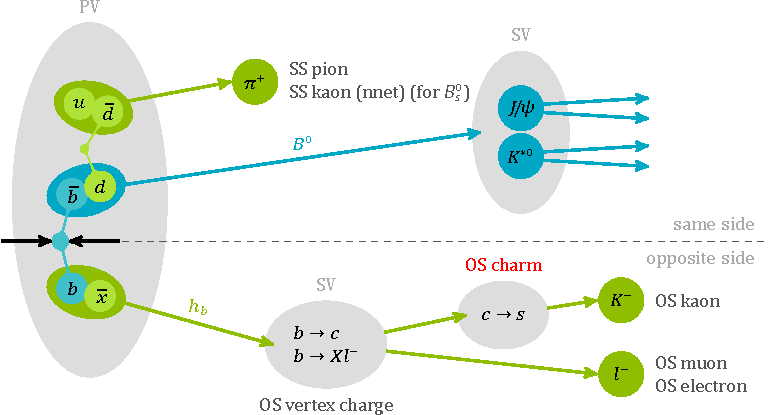
\includegraphics[width=\textwidth]{FTScheme/FlavourTaggerScheme.pdf}
\end{center}
\vspace{-0.6em}
Each tagger provides a decision $d$ on the initial flavour \newline(“tag”) and a probability to be wrong,  $\eta$.\\[0.3cm]
%\begin{itemize}
%\setlength\itemsep{0.01em}
%\item a decision on the initial flavour ("tag")
%\item an estimate to be wrong ($\eta$)
%\end{itemize}
\vspace{-0.75em}
\textbf{Flavour Tagging characteristics}
\vspace{0.1em}
\begin{itemize}
\item \textbf{mistag} \\[0.04cm] 
fraction of events with a wrong tagging decision
\begin{equation*}
\hspace{-1.6em}
\omega=\frac{N_{\text{wrong}}}{N_{\text{right}}+N_{\text{wrong}}}
\end{equation*}
\vspace{-1.1em}
\item \textbf{tagging efficiency} \\[0.04cm] 
fraction of events with a tagging decision
\begin{equation*}
\hspace{-1.6em}
\varepsilon_\text{tag}=\frac{N_{\text{right}}+N_{\text{wrong}}}{N_{\text{all}}}
\end{equation*}
\vspace{-1.1em}
\item \textbf{effective tagging efficiency} \\[0.04cm] 
represents the statistical reduction factor of a sample in a tagged analysis
\vspace{-0.3em}
\begin{equation*}
\hspace{-1.6em}
\vspace{0.5em}
\varepsilon_\text{eff}=\varepsilon_\text{tag}\left(1-2\omega\right)^2
\end{equation*}
\end{itemize}
%$N_R$/$N_W$/$N_U$ $:=$ number of correctly/incorrectly/untagged events.
%where $R$,$W$,$U$ are the number of correctly tagged, incorrectly tagged and untagged events. The tagging algorithms were developed and studied simulated events. (??) (REF)\\


}

% !TEX root = poster.tex
\headerbox{\textbf{Calibration}}{name=calib,column=0,row=1,below=basics,above=bottom}{
\textbf{Mistag calibration}
\vspace{-0.6em}
\begin{center}
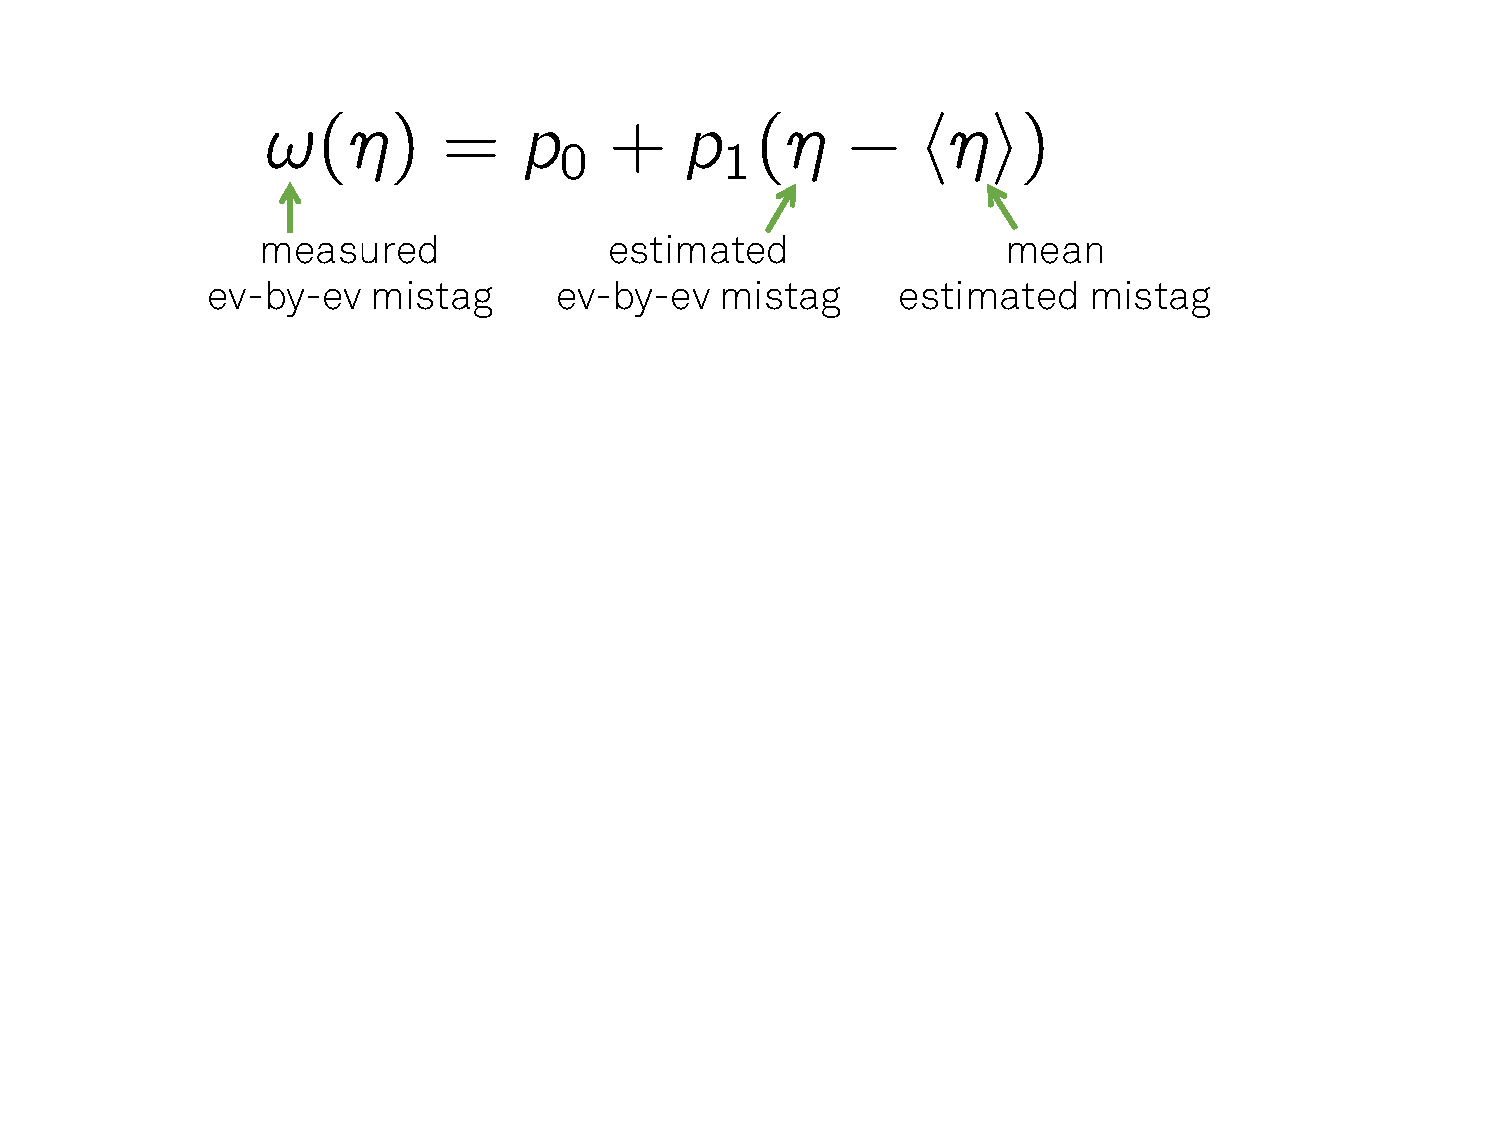
\includegraphics[width=0.75\textwidth]{figures/Calibration.pdf}
\end{center}
\vspace{-0.45em}
Several flavour-specific decay channels are used
\vspace{-0.5em}
\begin{itemize}
\setlength\itemsep{0.01em}
\item \BuToJPsiKp, $\Bu \rightarrow \D^0 \pi^+$ \\[0.05cm]
charged channels: extract $\omega$ by comparing tag decision with charge of final state
\item \BdToJPsiKst, \BdToDstarmunu, $\Bs \rightarrow D_s^- \pi^+$, ...\\[0.05cm]
neutral channels: full time-dependent analysis to extract $\omega$ from the mixing asymmetry 
%\vspace{-0.1em}
\begin{equation*}
\mathcal{A}_{\text{mix}}(t) = (1-2\omega)\cos (\Delta m_{d/s} t)
\end{equation*}
\end{itemize}
\vspace{-1.8em}
\begin{center}
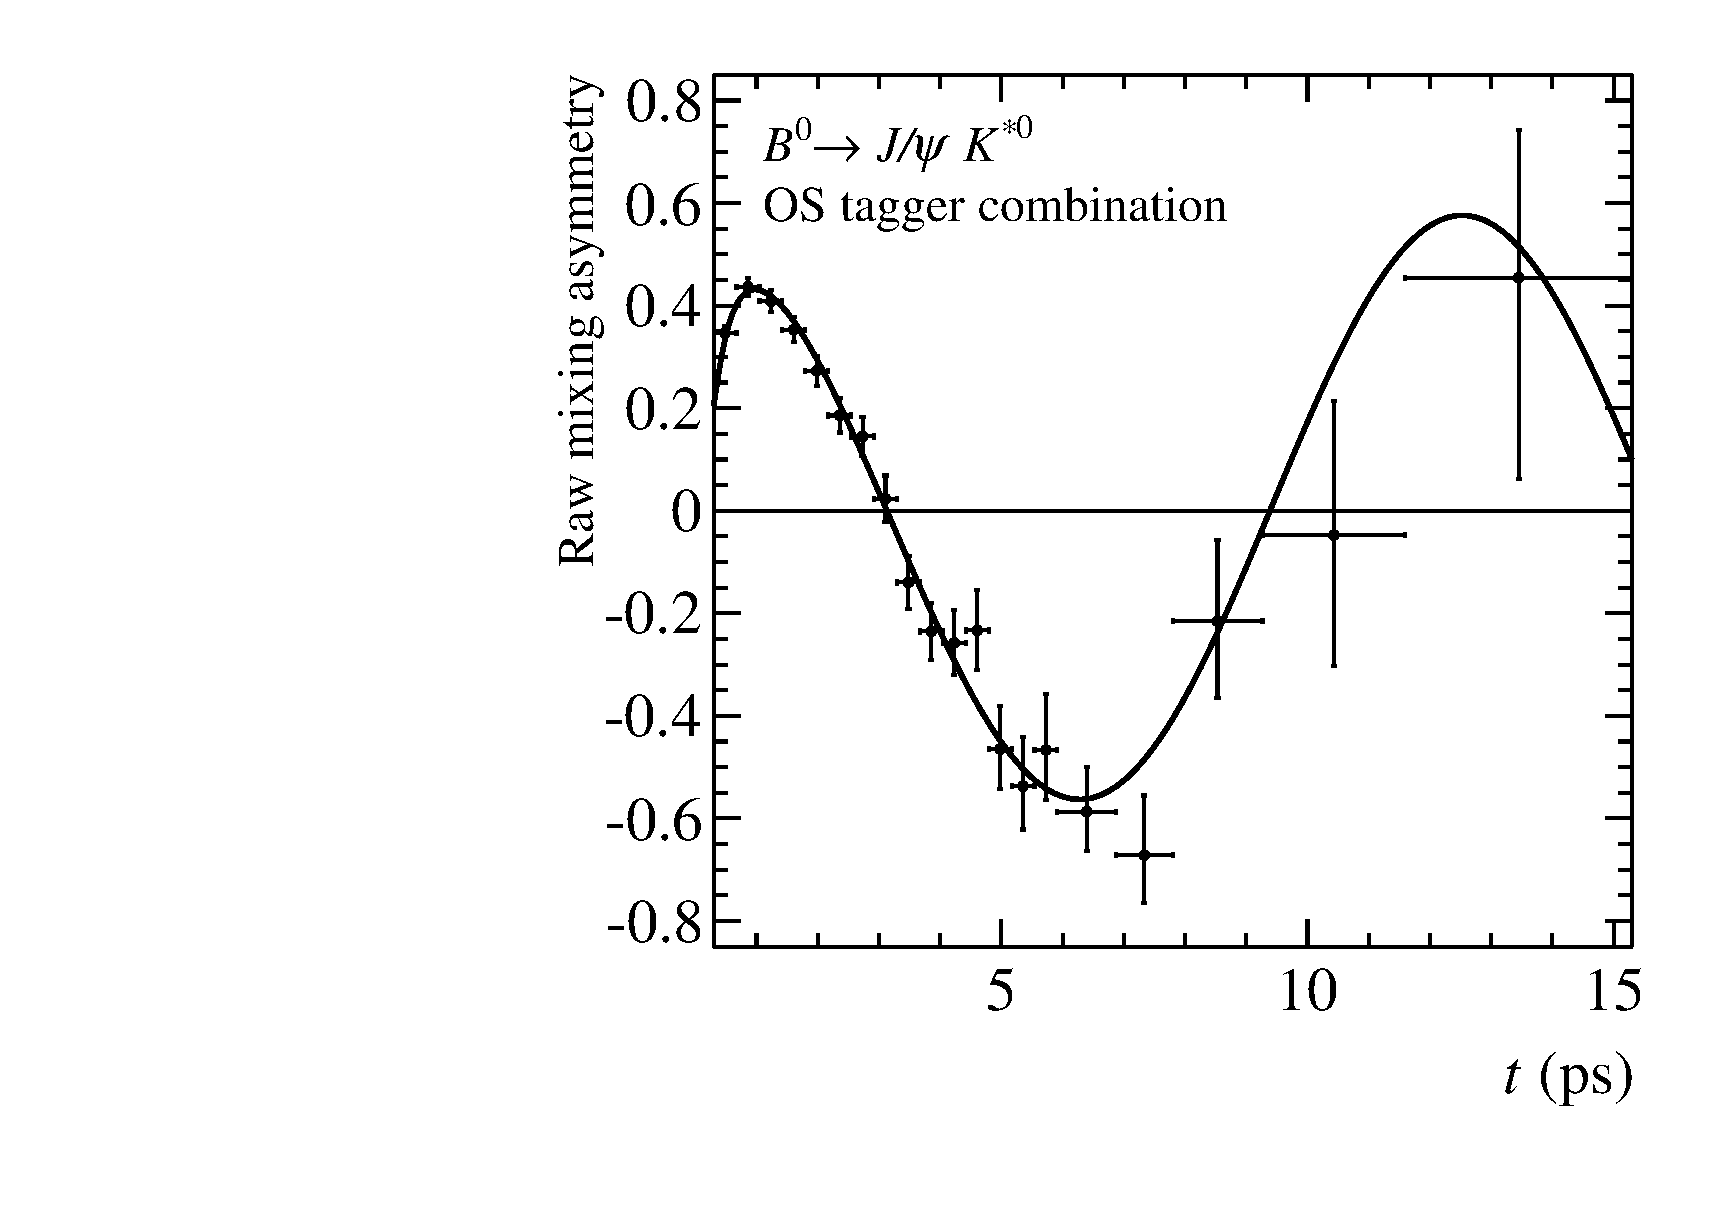
\includegraphics[width=0.475\boxwidth]{KstAsym.pdf}
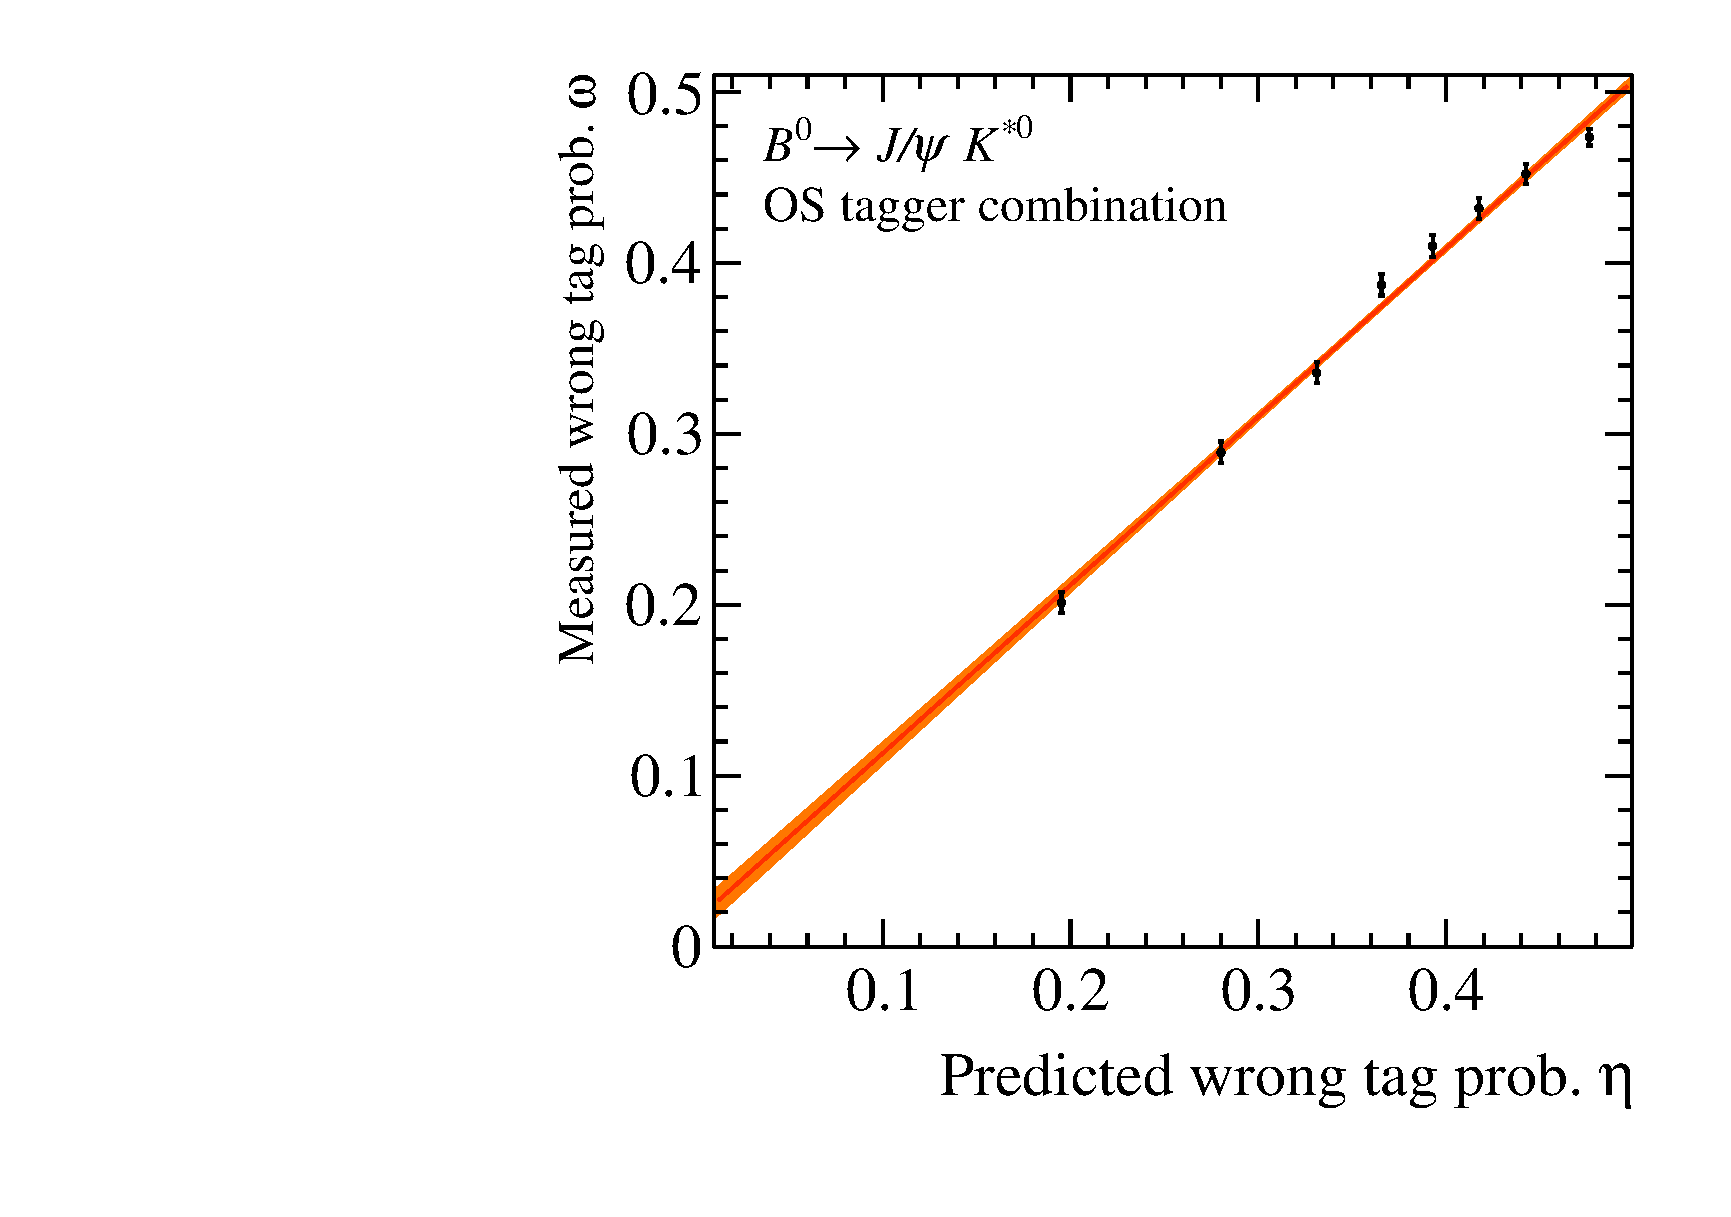
\includegraphics[width=0.475\boxwidth]{Bd2JpsiKst-Kst-OST-8ScalingFunction_raw.pdf}
\end{center}

}
% !TEX root = poster.tex
\headerbox{\textbf{Flavour Tagging in Run I}}{name=run1,column=1,span=2,row=0}{
\begin{minipage}{0.474\boxwidth}
\textbf{Usage in analyses}\\[-0.45em]
\vspace{-0.5em}
\begin{itemize}
\setlength\itemsep{0.01em}
\vspace{-0.3em}
\item one calibration per tagger valid for all channels
\item systematic uncertainties from
\begin{itemize}
\setlength\itemsep{0.01em}
\setlength{\itemindent}{-.11in}
\vspace{-0.4em}
\item[${\color{tu_gruen}-}$] calibration methods
\item[${\color{tu_gruen}-}$] results in different control channels 
\end{itemize}
\vspace{-0.4em}
\item  ``ad-hoc'' calibration using best-suited control channels for analyses dominated by FT uncertainty %(\BdToJPsiKS)
\end{itemize}
%\vspace{-0.9em}
%\begin{center}
%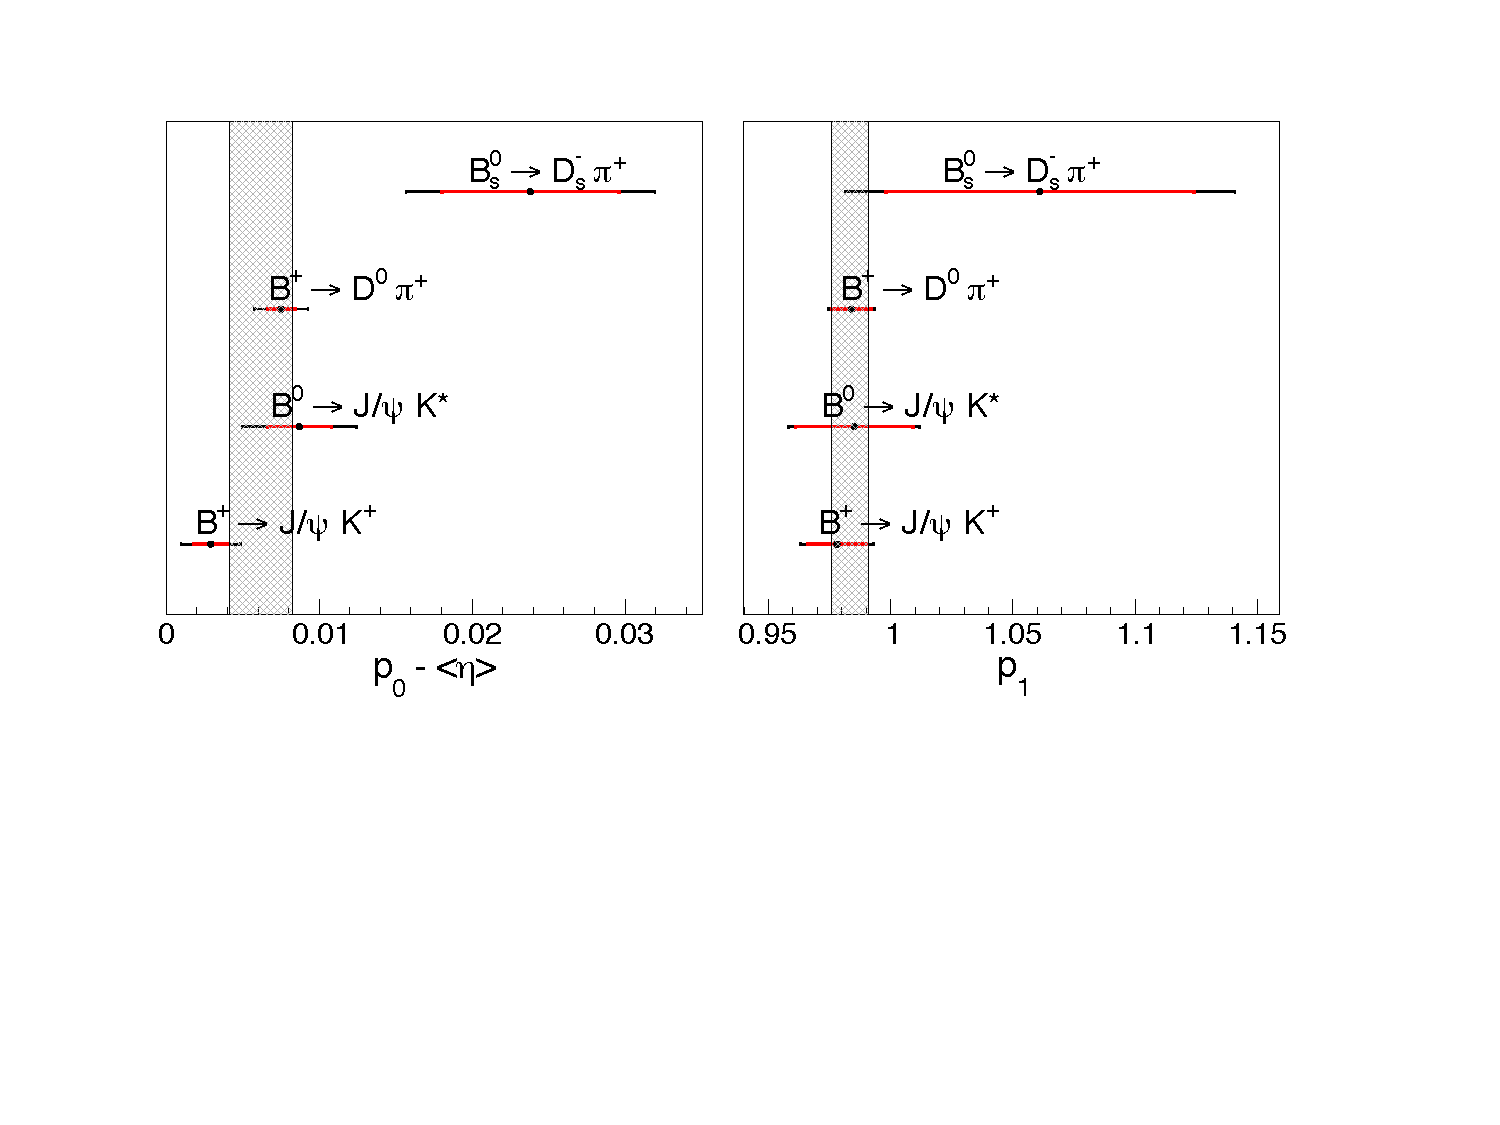
\includegraphics[width=0.466\boxwidth]{graphP0P1.pdf}
%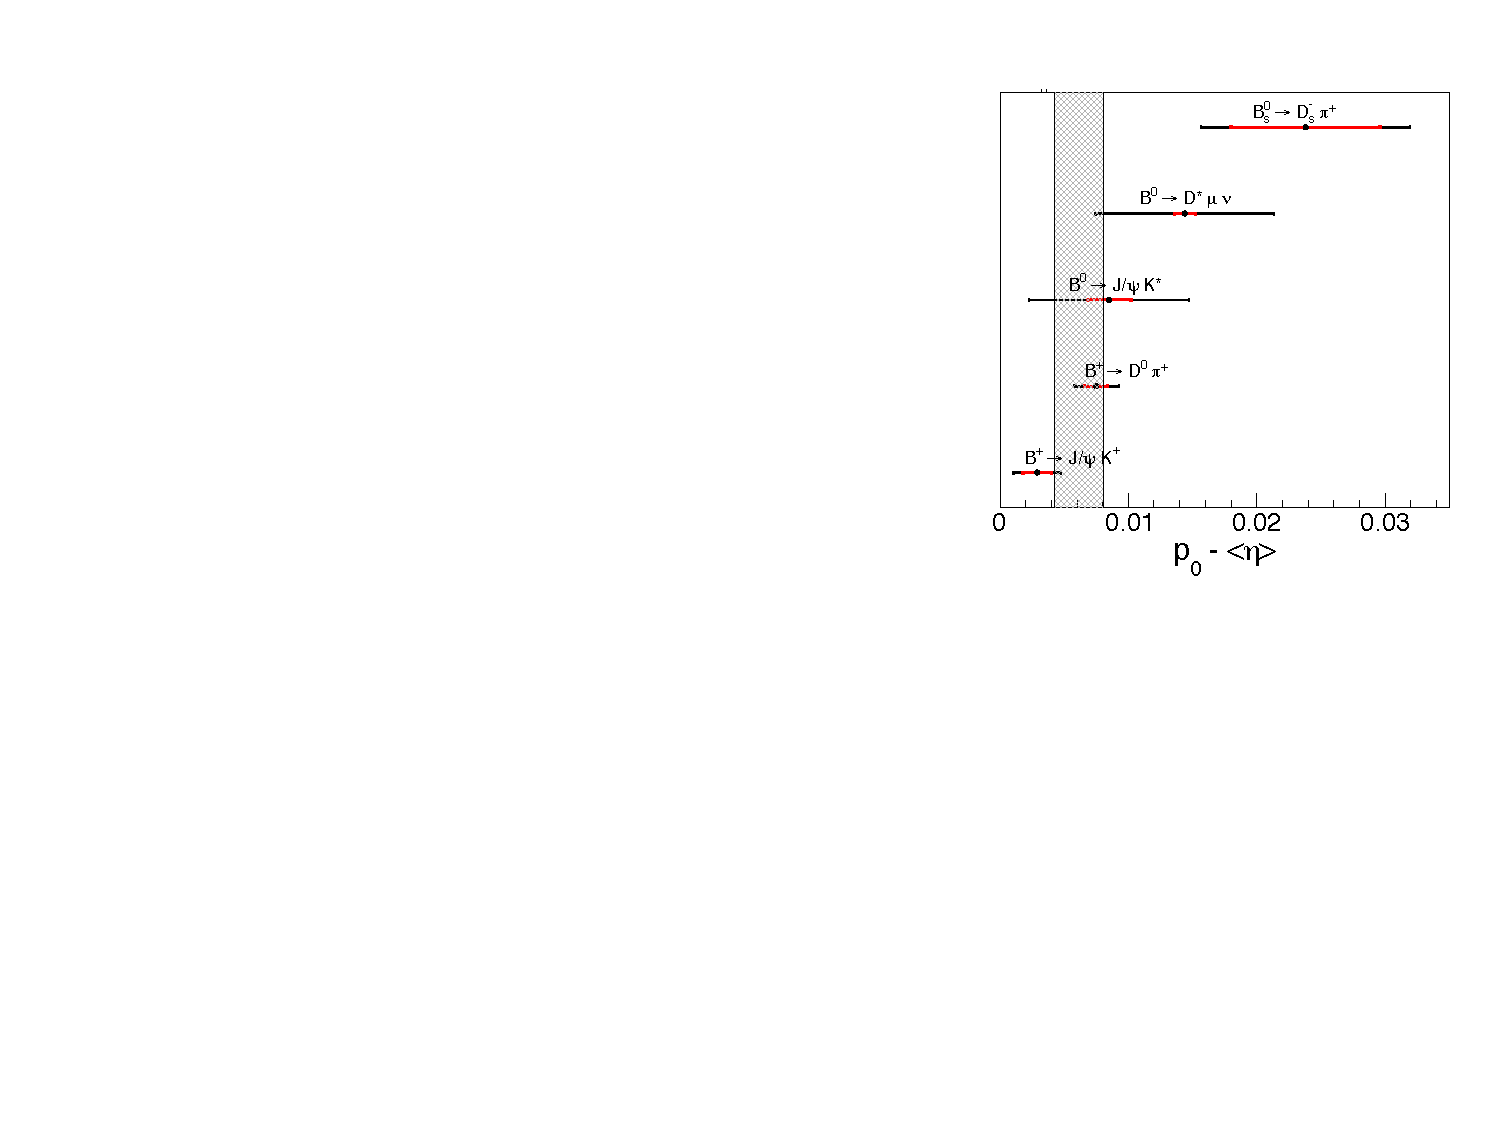
\includegraphics[width=0.233\boxwidth]{portability_p0.pdf}
%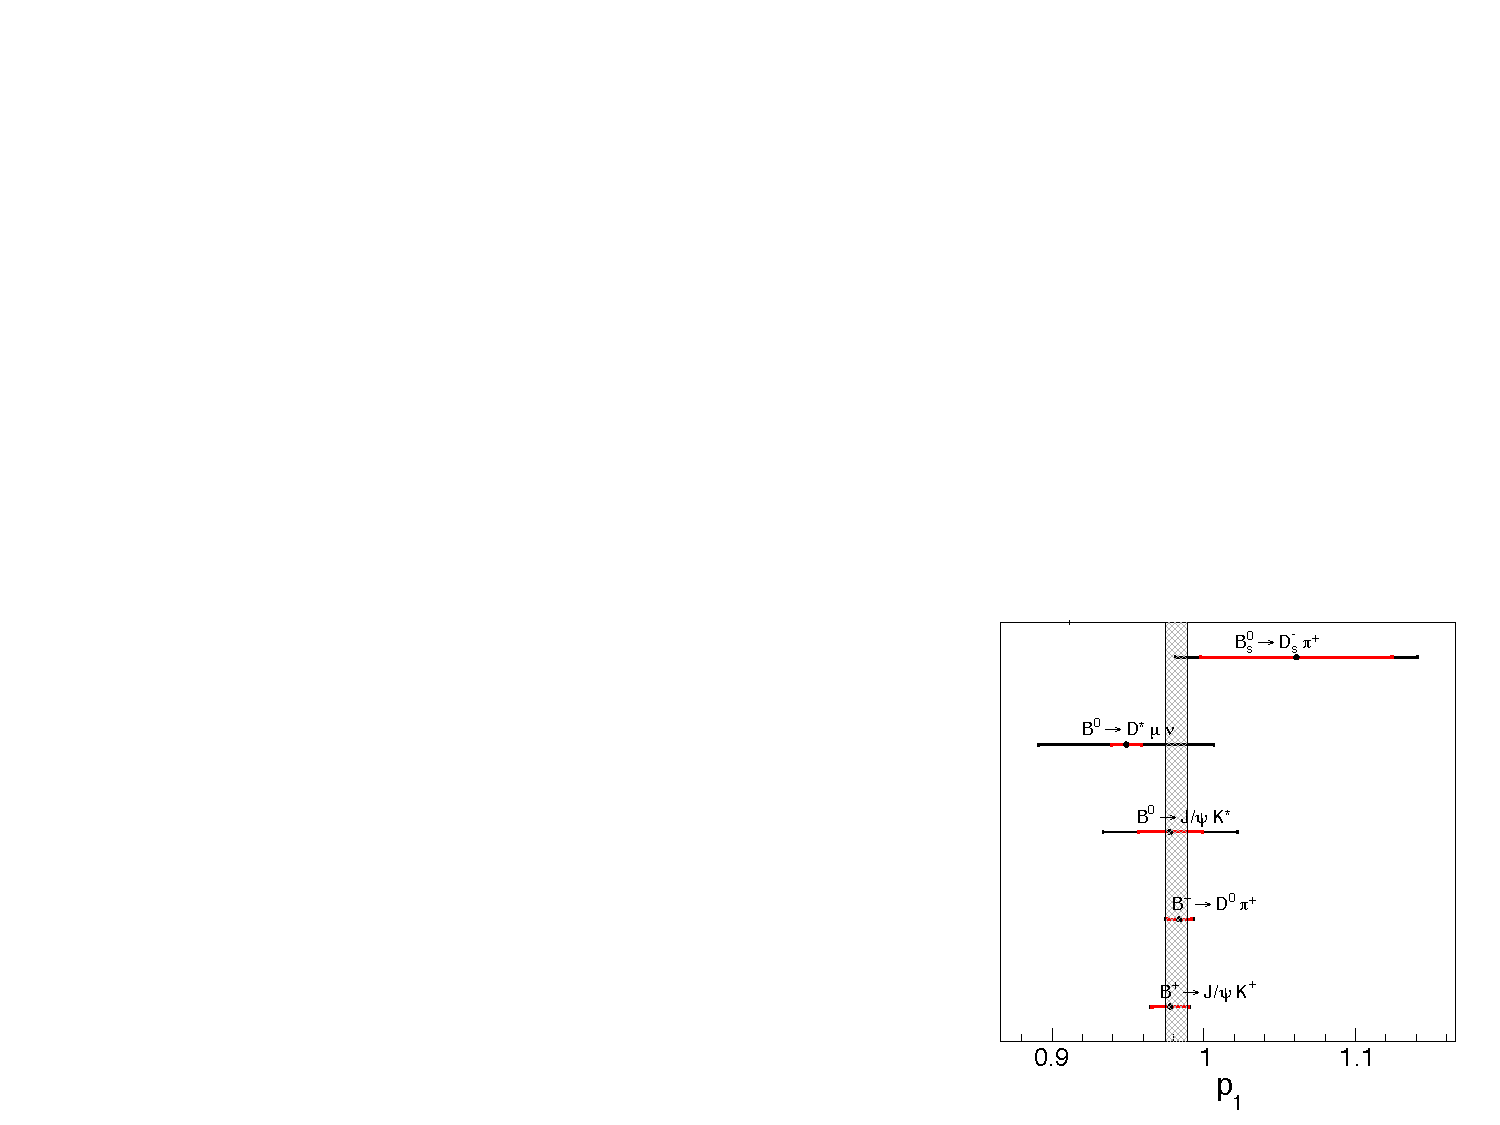
\includegraphics[width=0.233\boxwidth]{portability_p1.pdf}
%\end{center}
\vspace{0.45em}
\textbf{Highlights of flavour-tagged measurements}
\vspace{-0.3em}
\begin{itemize}
\item\textbf{Measurements of $\phi_s$}

\vspace{-1.1em}
\begin{center}
%\hspace{-1.5em}
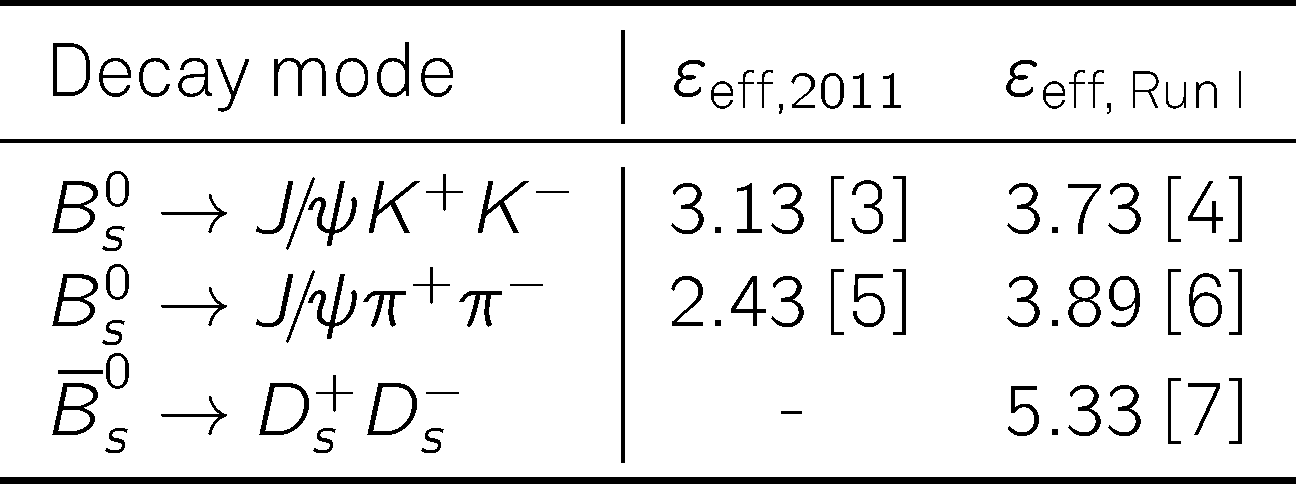
\includegraphics[width=0.802\textwidth]{figures/Bs2JpsiKK3.pdf}
\end{center}
\vspace{-2.3em}

	\begin{itemize}
	\setlength\itemsep{0.01em}
	\setlength{\itemindent}{-.11in}
	%\item[${\color{tu_gruen}-}$] analysis on \num{2011} data: $\varepsilon_\text{eff}=\SI{3.13}{\%}$ [3] 
	%\item[${\color{tu_gruen}-}$] full Run I analysis: $\varepsilon_\text{eff}=\SI{3.73}{\%}$ [4] 
	\item[${\color{tu_gruen}-}$] newest analyses profited from: 
	\setlength{\itemindent}{.05in}
	\item[${\color{tu_gruen}\rightarrow}$] including SS kaon nnet tagger
	\item[${\color{tu_gruen}\rightarrow}$] re-optimisation of OS algorithms
	\end{itemize}
	
\vspace{-2.8em}
\begin{center}
%\hspace{-1.5em}
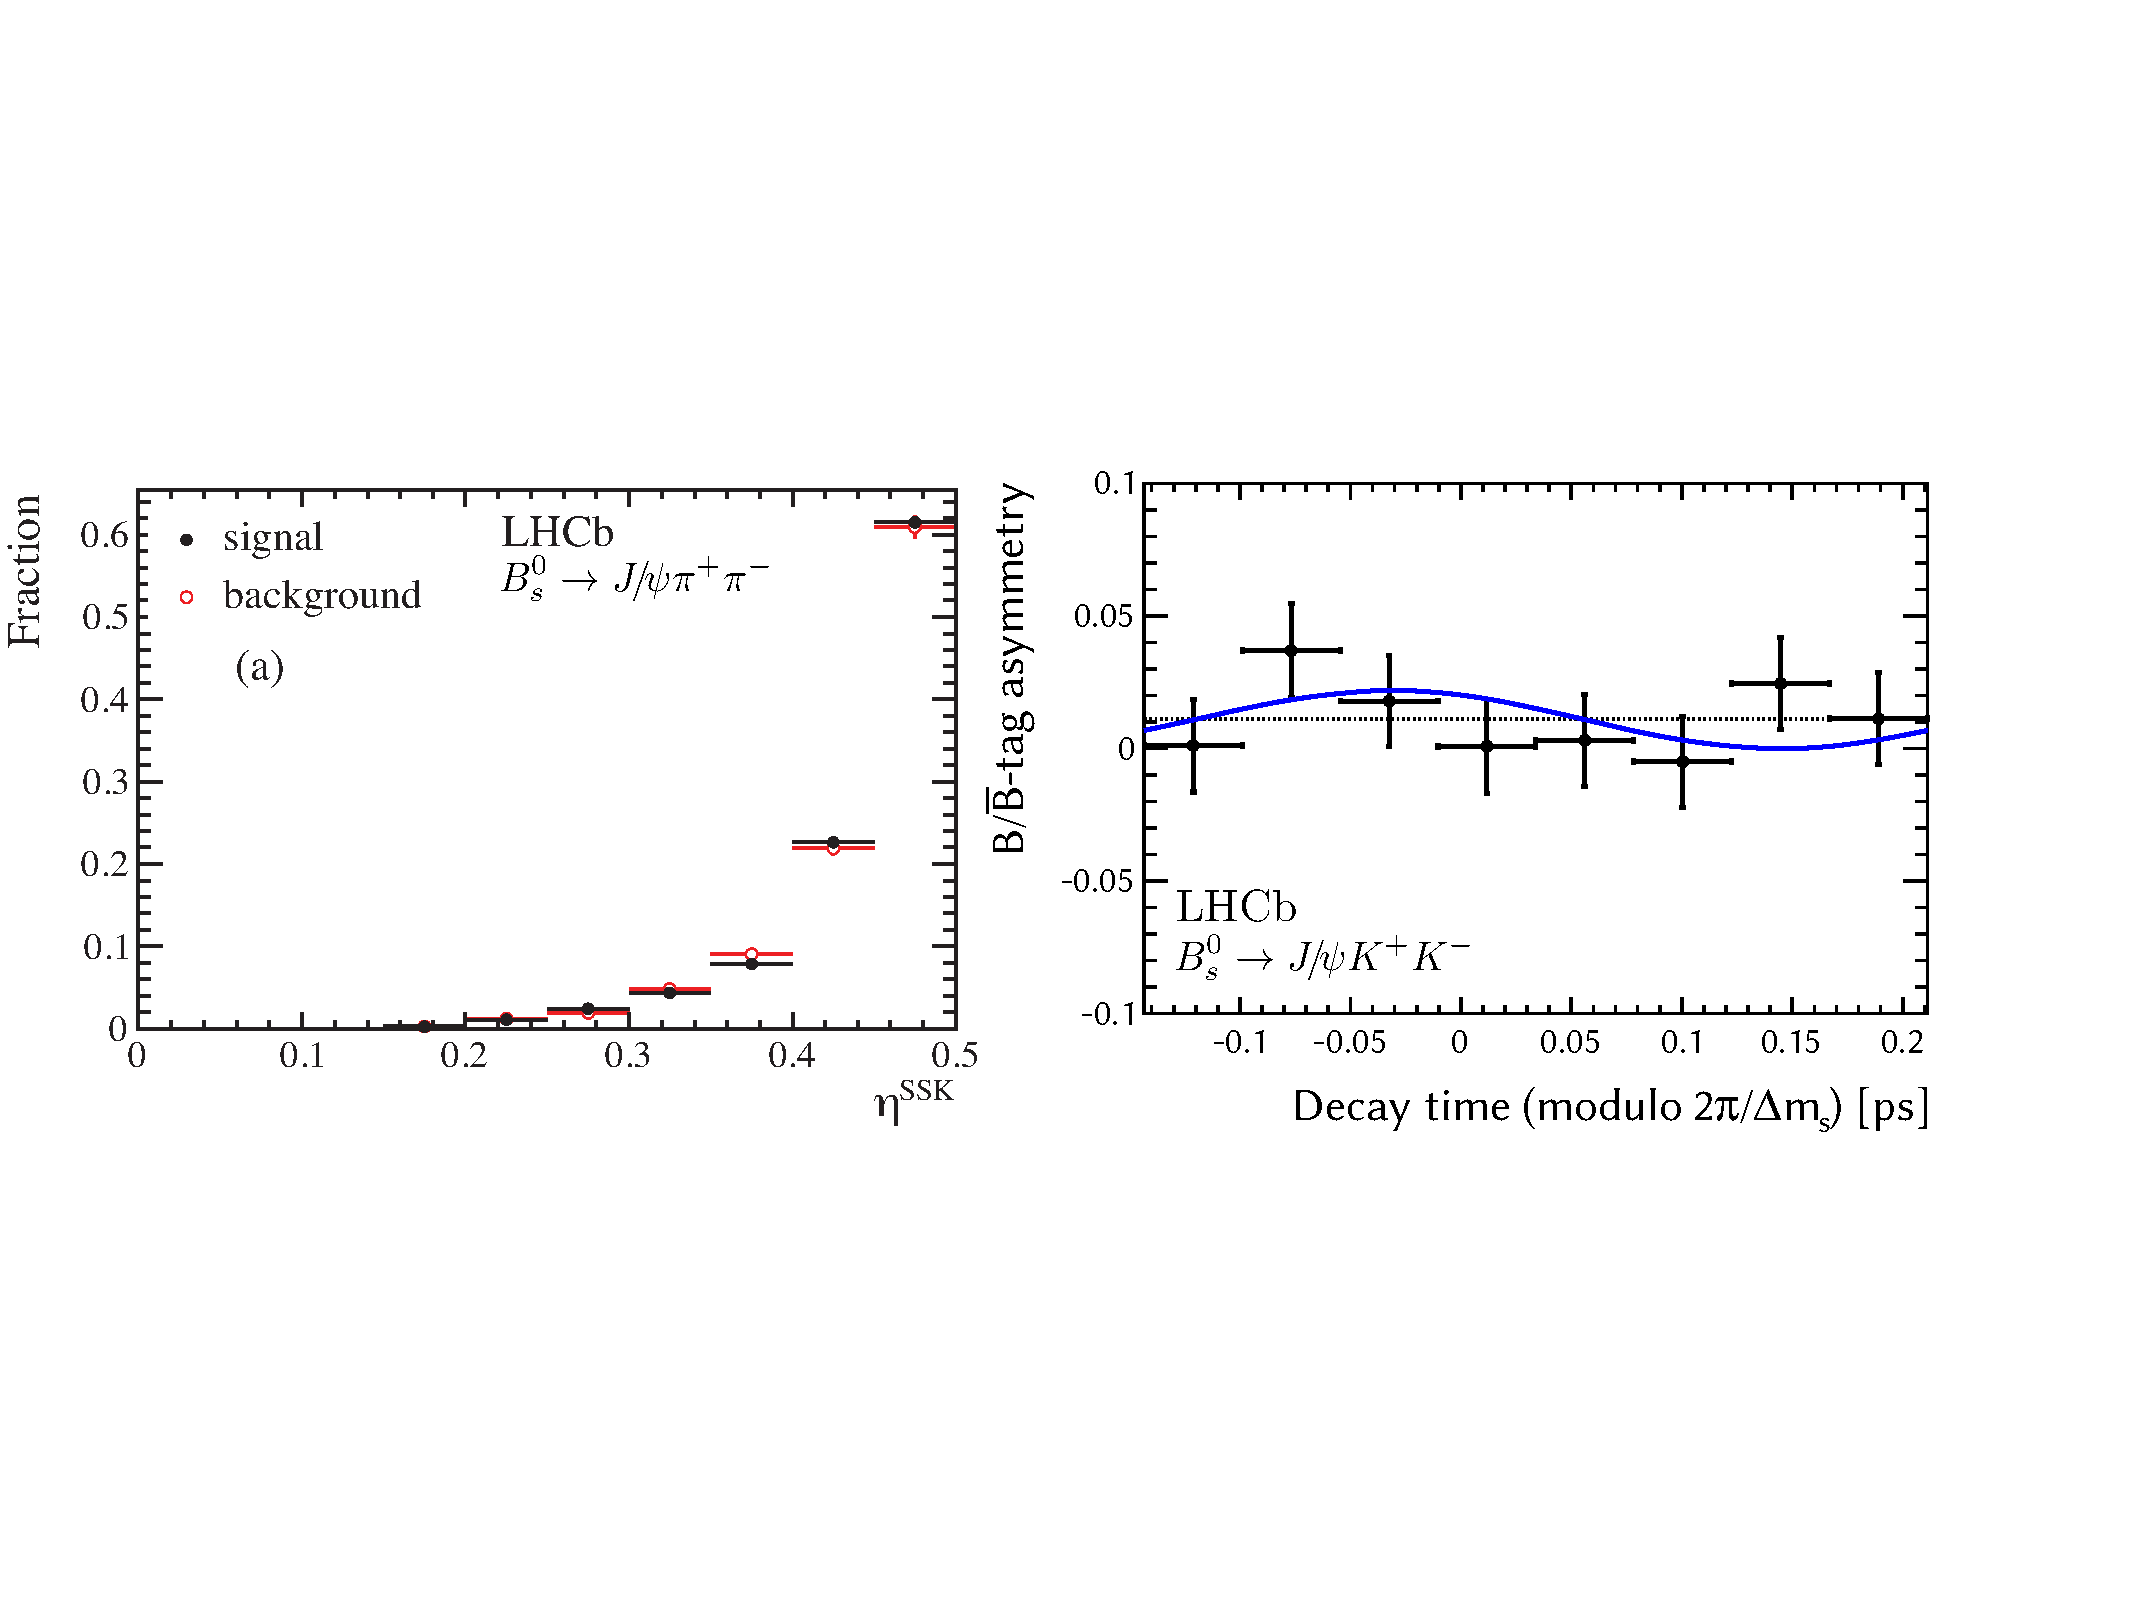
\includegraphics[width=0.474\boxwidth]{figures/Bs2JpsiKK4.pdf}
\end{center}
\vspace{-1.05em}
	
\setlength\itemsep{-0.21em}
\item\textbf{\CP violation in \BsToDsK}

\vspace{-2.1em}
\begin{flushleft}
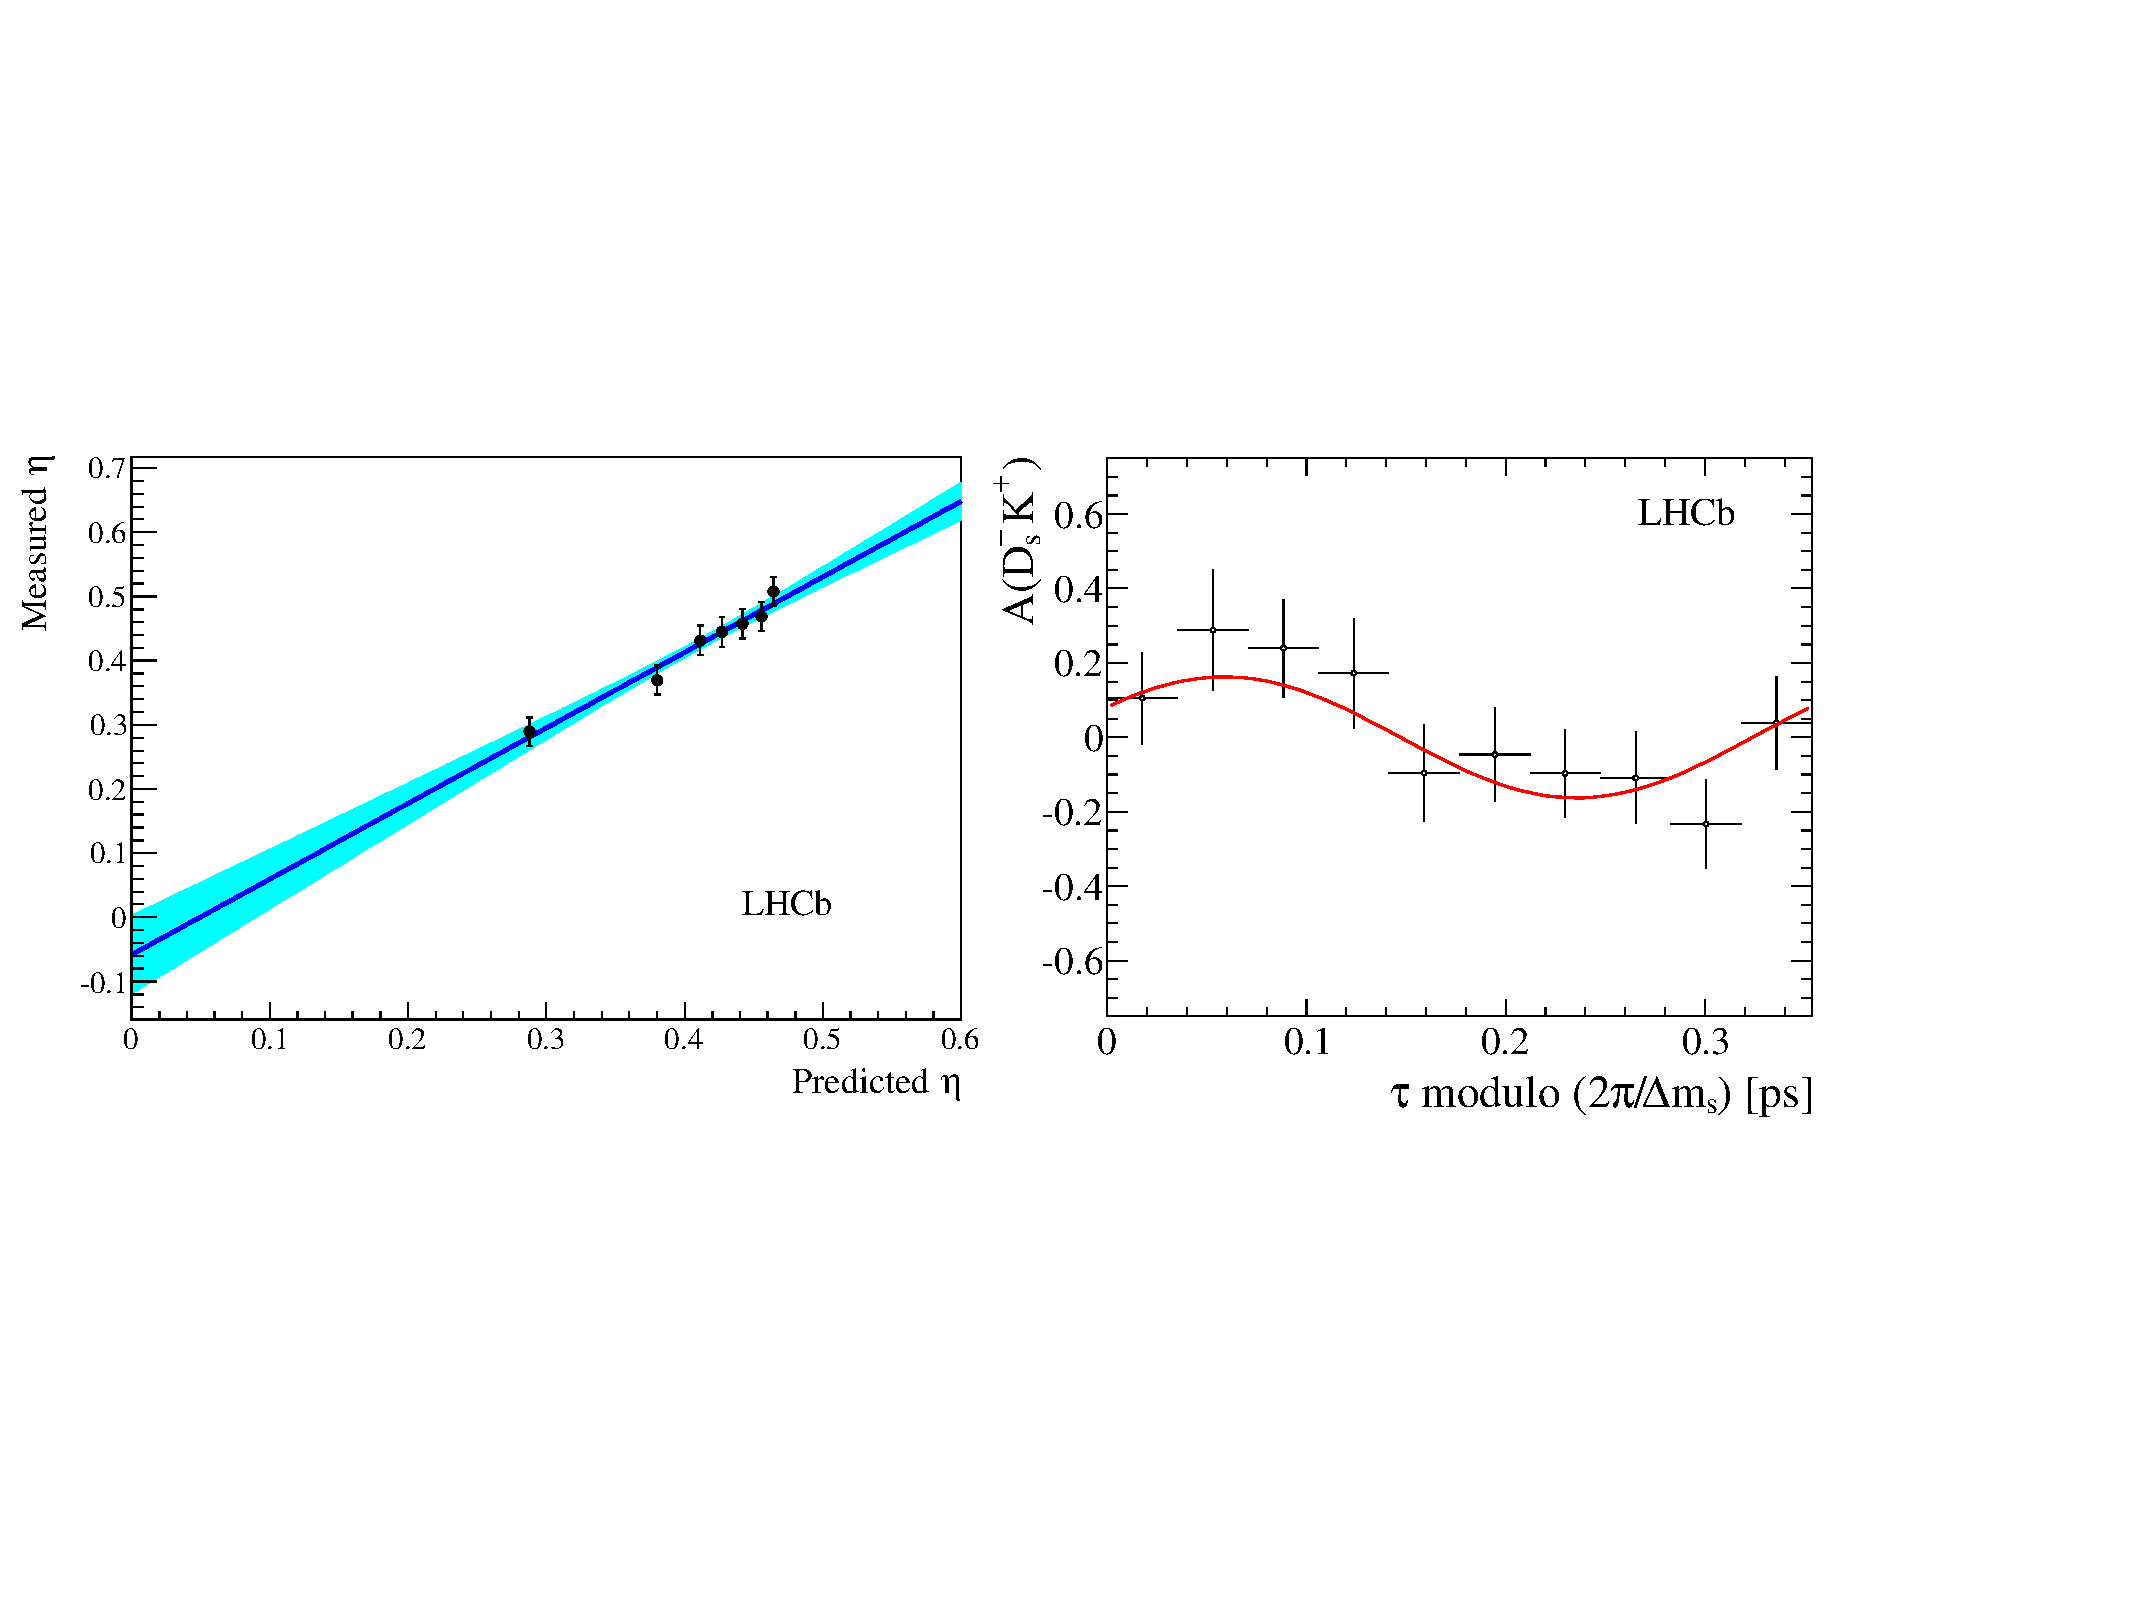
\includegraphics[width=0.474\boxwidth]{CPV_DsK2.pdf}
\end{flushleft}
\vspace{-2.8em}

	\begin{itemize}
	\setlength\itemsep{0.01em}
	\setlength{\itemindent}{-.11in}
	\item[${\color{tu_gruen}-}$] analysis on \num{2011} data: $\varepsilon_\text{eff}=\SI{5.07}{\%}$
	\item[${\color{tu_gruen}-}$] SS kaon nnet adds more than \SI{1.3}{\%} to $\varepsilon_\text{eff}$ [8]
	\end{itemize}
\end{itemize}
\end{minipage}
\vspace{0.7em}
\hfill
\begin{minipage}{0.474\boxwidth}
\vspace{-0.3em}
\begin{itemize}
\item\textbf{\CP violation in \BdToJPsiKS ($\sin2\beta$)}
\vspace{-0.2em}
	\begin{itemize}
	\setlength\itemsep{0.01em}
	\setlength{\itemindent}{-.11in}
	\item[${\color{tu_gruen}-}$] analysis on \num{2011} data: $\varepsilon_\text{eff}=\SI{2.38}{\%}$ [9]
	\item[${\color{tu_gruen}-}$] full Run I analysis: $\varepsilon_\text{eff}=\SI{3.02}{\%}$ [10] 
	\setlength{\itemindent}{.05in} 
	\item[${\color{tu_gruen}\rightarrow}$] SS pion tagger adds more than \SI{0.376}{\%} to $\varepsilon_\text{eff}$ 
	\end{itemize}
	
\vspace{-1.7em}
\begin{center}
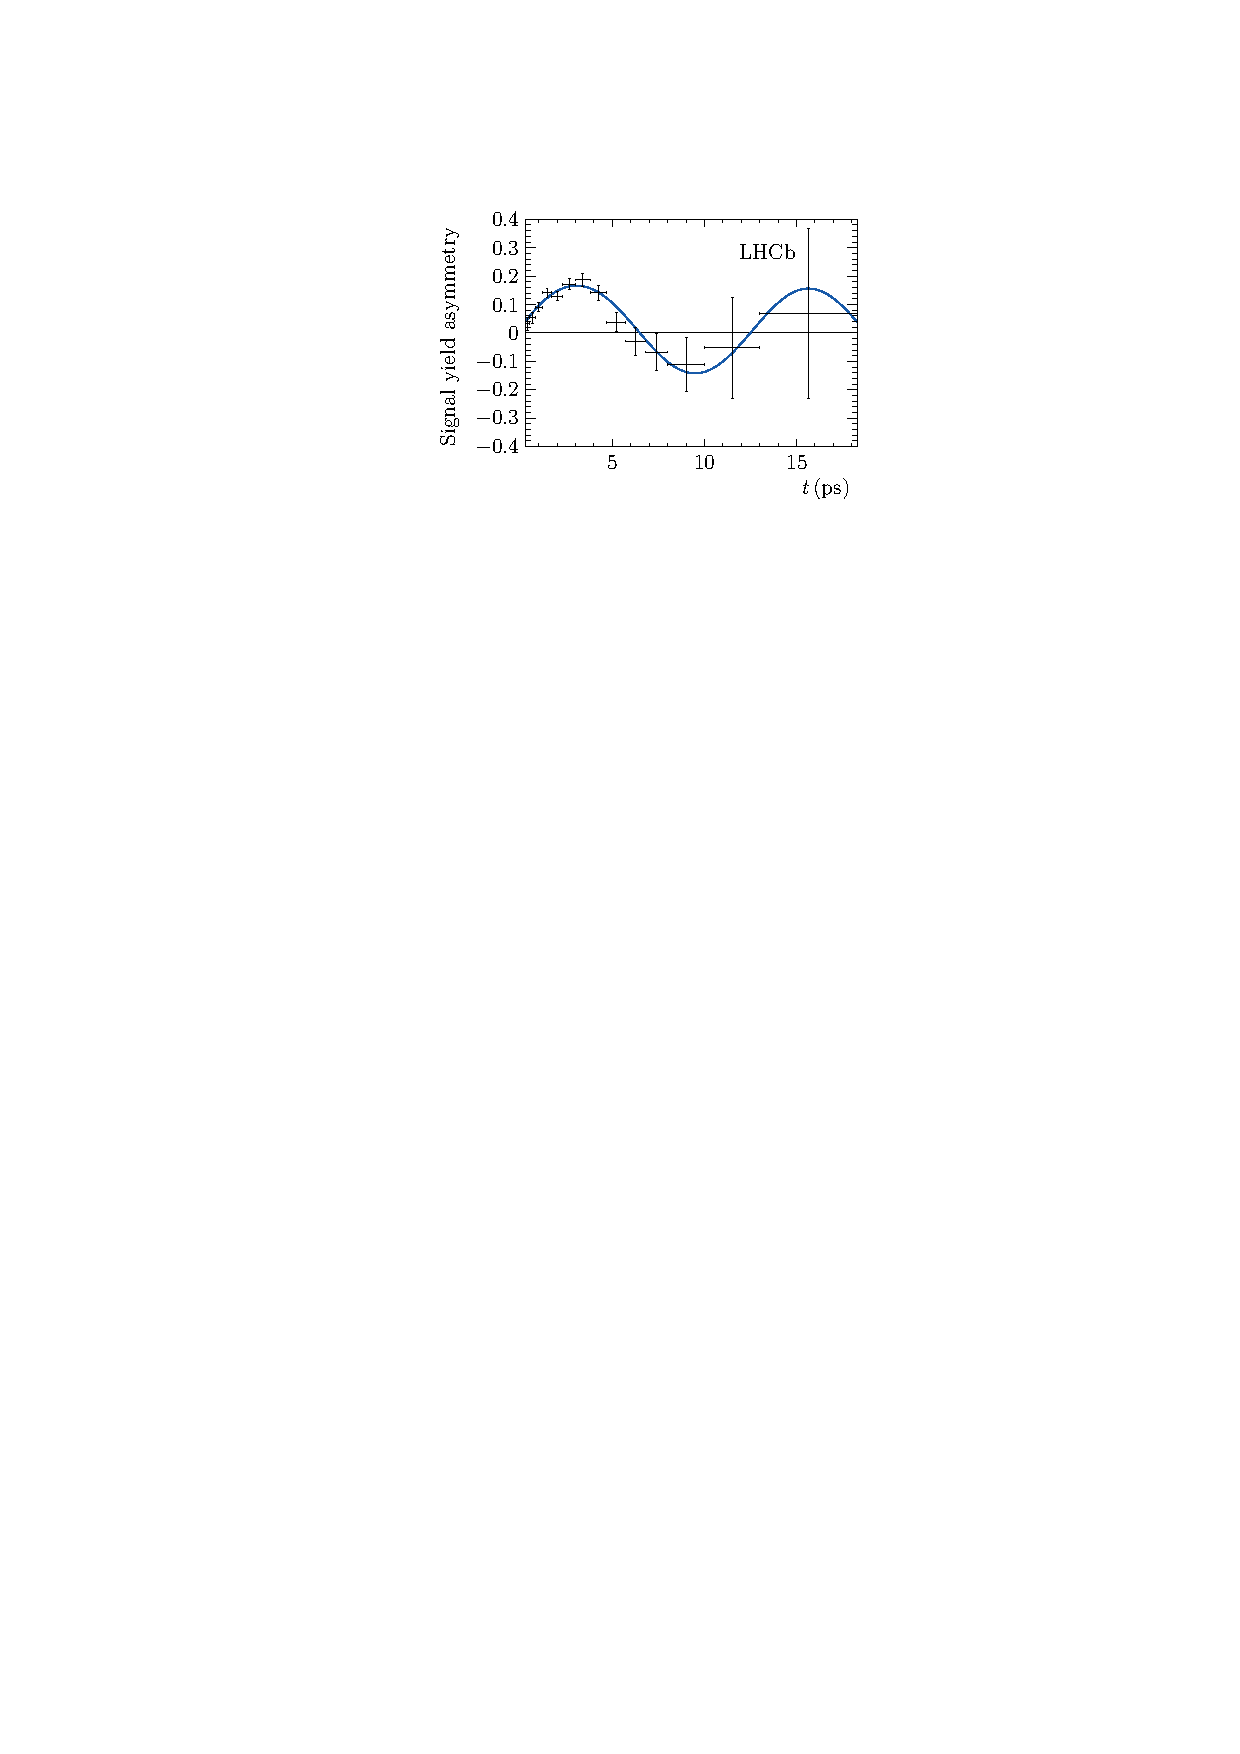
\includegraphics[width=0.335\boxwidth]{CPV_sin2beta.pdf}
\end{center}
\vspace{-2.5em}

	\begin{itemize}
	\setlength{\itemindent}{-.11in}
	\setlength\itemsep{0.01em}
	\item[${\color{tu_gruen}-}$] precision analysis \hspace{0.1em}${\color{tu_gruen}\rightarrow}$ ``ad-hoc'' FT calibration
	\setlength{\itemindent}{.05in}
	%\item[${\color{tu_gruen}\rightarrow}$] smaller uncertainties from FT 
	\item[${\color{tu_gruen}\rightarrow}$] OS algorithms calibrated with \BuToJPsiKp 
	\item[${\color{tu_gruen}\rightarrow}$] SS pion calibrated with \BdToJPsiKst
	\end{itemize}
%\vspace{0.1em}
%\item\textbf{\BsTophiphi}

\vspace{-0.1em}
\item\textbf{\CP violation in \BsToJPsiKS}
	\begin{itemize}
	\setlength\itemsep{0.01em}
	\setlength{\itemindent}{-.11in}
	\item[${\color{tu_gruen}-}$] not possible to exclude \Bd events in selection
	\end{itemize}
	
\vspace{-2.1em}
\begin{flushleft}
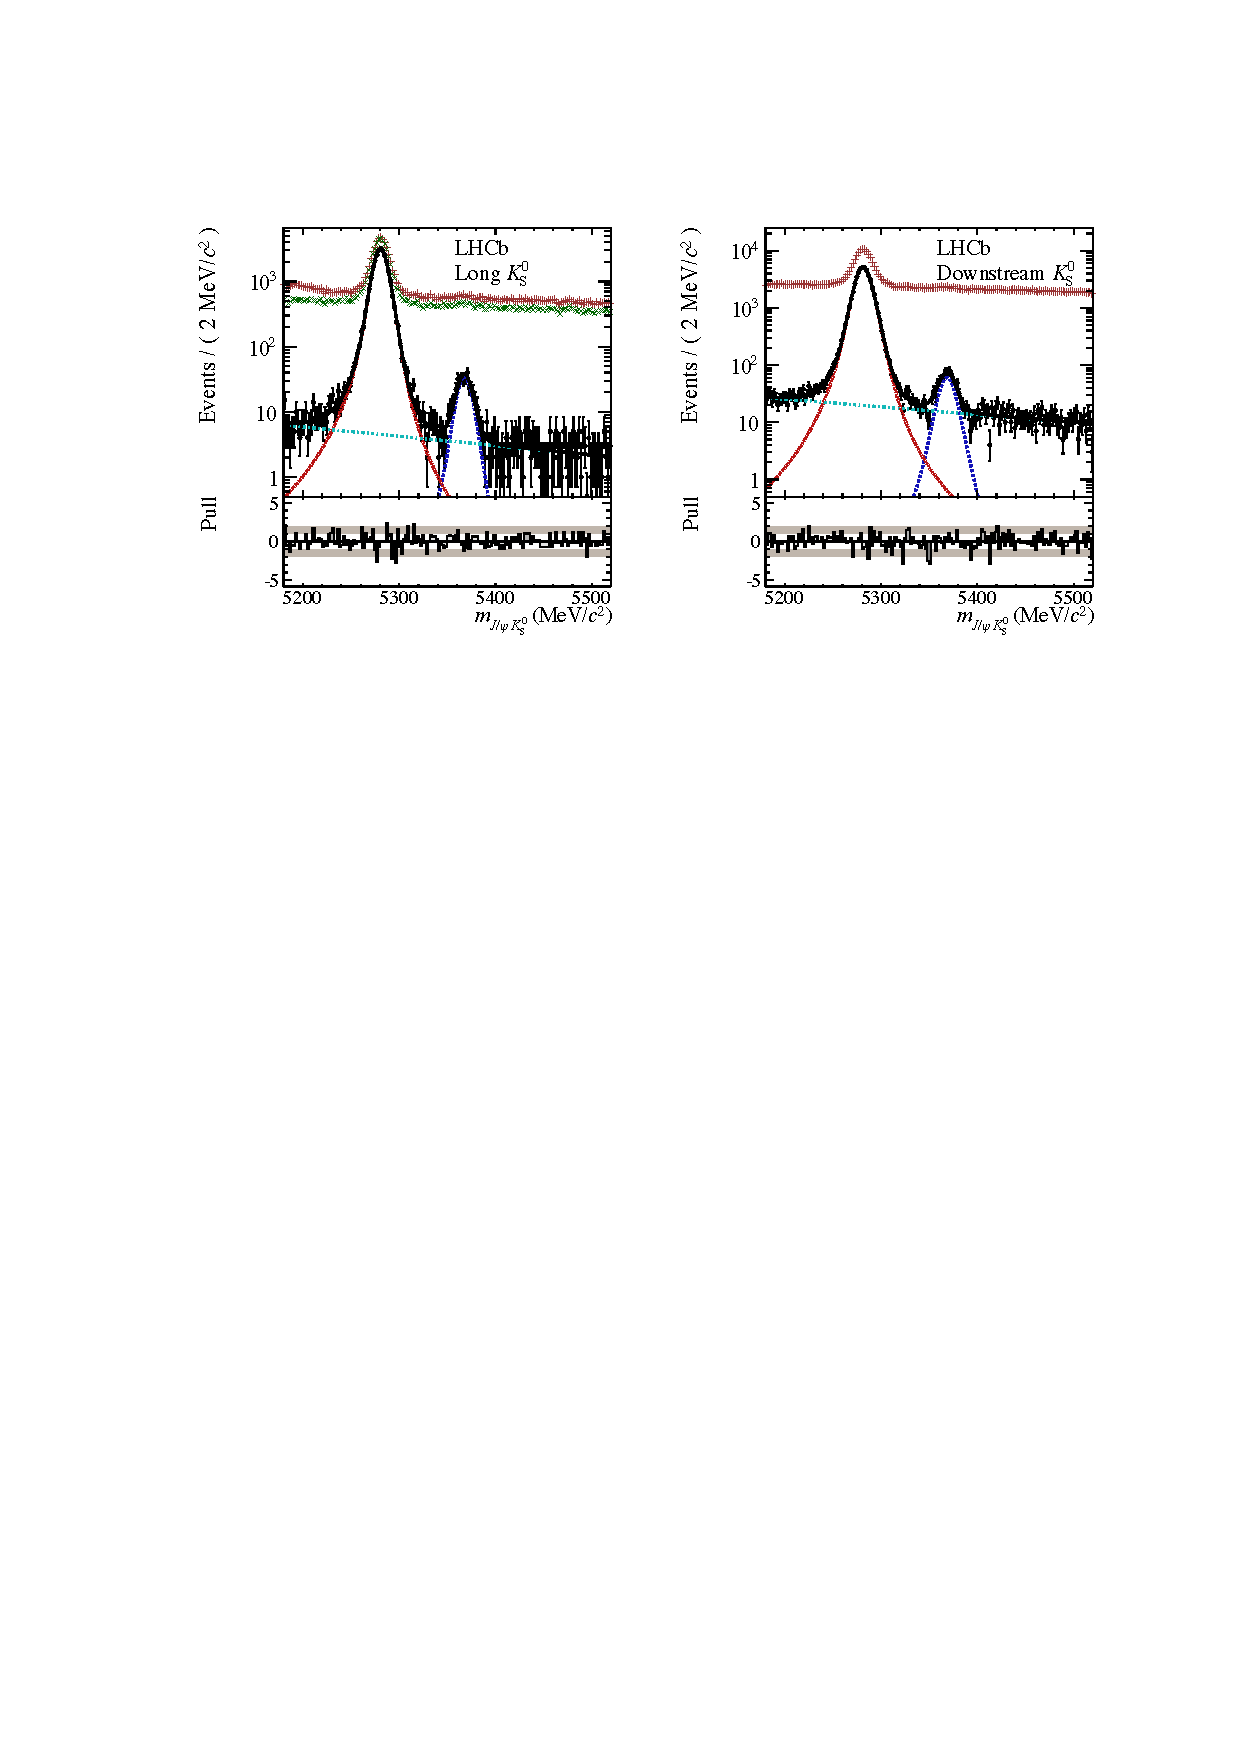
\includegraphics[width=0.45\boxwidth]{CPV_BsJpsiKS.pdf}
\end{flushleft}
\vspace{-2.2em}

	\begin{itemize}
	\setlength\itemsep{0.01em}
	\setlength{\itemindent}{-.11in}
	\item[${\color{tu_gruen}-}$] \Bs events: $\varepsilon_\text{eff}=\SI{4.00}{\%}$ [11]
	\item[${\color{tu_gruen}-}$] \Bd events: $\varepsilon_\text{eff}=\SI{2.62}{\%}$ [11]
	\setlength{\itemindent}{.05in}
	\item[${\color{tu_gruen}\rightarrow}$] small tagging power of SS kaon for \Bd:
	%\item[${\color{tu_gruen}\rightarrow}$] origins of this effect:
	\setlength{\itemindent}{.10in}
	\item[${\color{tu_gruen}-}$] same-side protons misidentified as kaons
	\item[${\color{tu_gruen}-}$] kaons from same-side \Kstar(892)
	\vspace{-0.35em}
		\begin{itemize}[leftmargin=.05in]
		%\setlength{\itemindent}{.05in}
		\item[${\color{tu_gruen}\Rightarrow}$] kaons have opposite charge for \Bd:\\ tagging decision has to be inverted
		\end{itemize}
	\end{itemize}


%\item\textbf{Measurement of \dms with \BsToDspi}
%
%\vspace{-1.7em}
%\begin{center}
%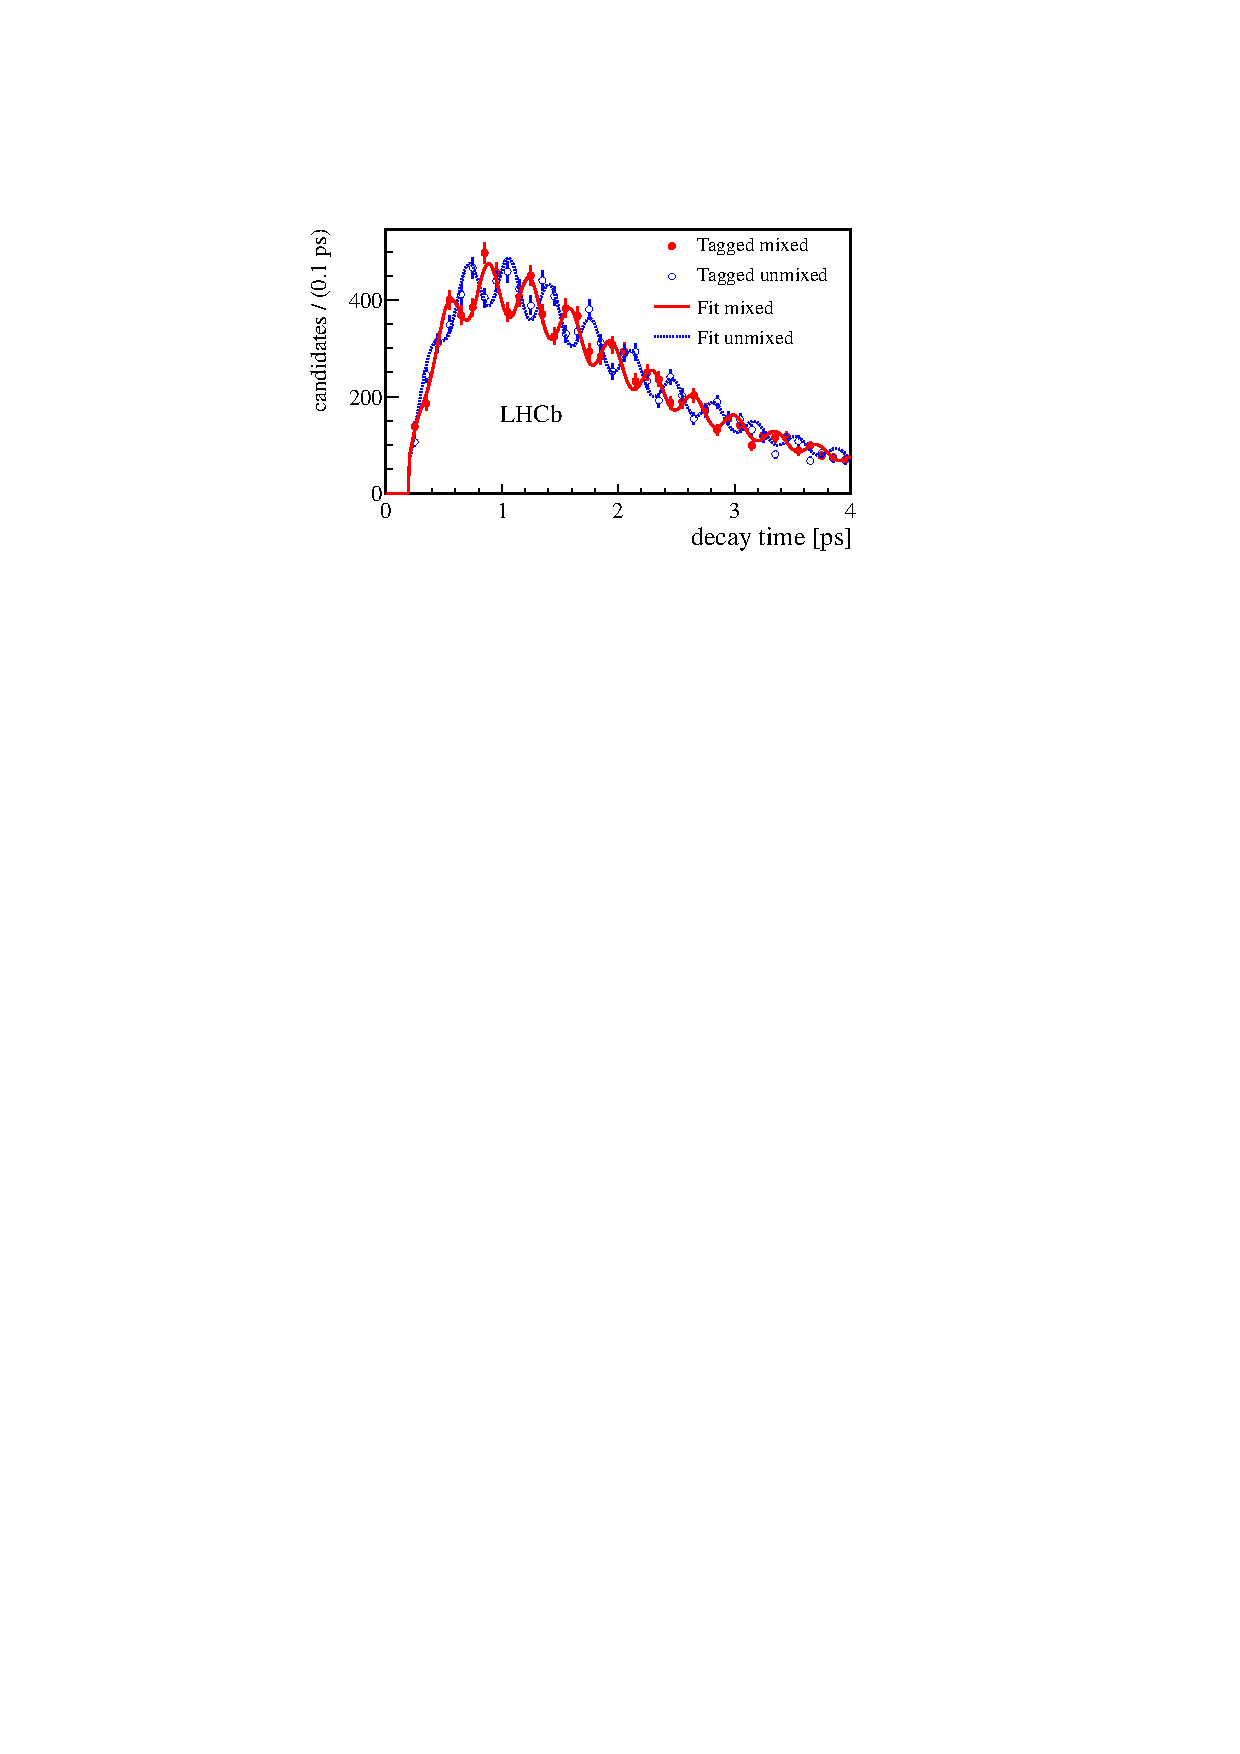
\includegraphics[width=0.266\boxwidth]{Bs_mixing1.pdf}
%\end{center}
%\vspace{-2.5em}
%
%	\begin{itemize}
%	\item[${\color{tu_gruen}-}$] Decay rates: $e^{-\Gamma t}\left(...+\!d\cos\left(\Delta mt\right)\right)$
%	\end{itemize}
\end{itemize}

%\textbf{Overall performance improvements in Run I}
%\begin{itemize}
%\setlength\itemsep{0.01em}
%\vspace{-0.3em}
%\item OS tagging improved $\mathcal{O}$(15\%) 
%\item SS kaon tagging improved $\mathcal{O}$(40\%)
%\vspace{0.5em}
%\setlength{\itemindent}{.14in}
%\item[$\color{tu_gruen}\Rightarrow$] \textbf{Flavour Tagging has been a success in Run I}
%\end{itemize}
\end{minipage}
\vspace{-0.1em}
}

% !TEX root = poster.tex
%\headerbox{Recent Developments}{name=devs,column=1,row=1,below=run1,above=bottom}{
\headerbox{\textbf{Developments}}{name=devs,column=1,row=1,span=2,below=run1}{
\begin{minipage}{0.474\boxwidth}
\vspace{-2.72em}
\textbf{SS kaon calibration with excited \Bs states}
\vspace{-0.1em}
\begin{itemize}
\item SS kaon taggers calibrated with \BsToDspi only
\begin{itemize}
\setlength{\itemindent}{-.11in}
\item[${\color{tu_gruen}-}$] limited statistics
\item[${\color{tu_gruen}-}$] time-dependent analysis required
\end{itemize}
\vspace{-0.8em}
\item new idea: calibrate with $B_s^{**0}$ decays
%\setlength{\itemindent}{.05in}
%\item[${\color{tu_gruen}\Rightarrow}$] further control channel for SS kaon tagging
\begin{itemize}
\setlength\itemsep{0.01em}
\setlength{\itemindent}{-.11in}
\item[${\color{tu_gruen}-}$] narrow states
\item[${\color{tu_gruen}-}$] reconstruct in  $B_s^{**0}\to\Bp\Km$ decays
\item[${\color{tu_gruen}-}$] calibrate by counting, as in other charged modes 
\end{itemize}
\end{itemize}
\begin{center}
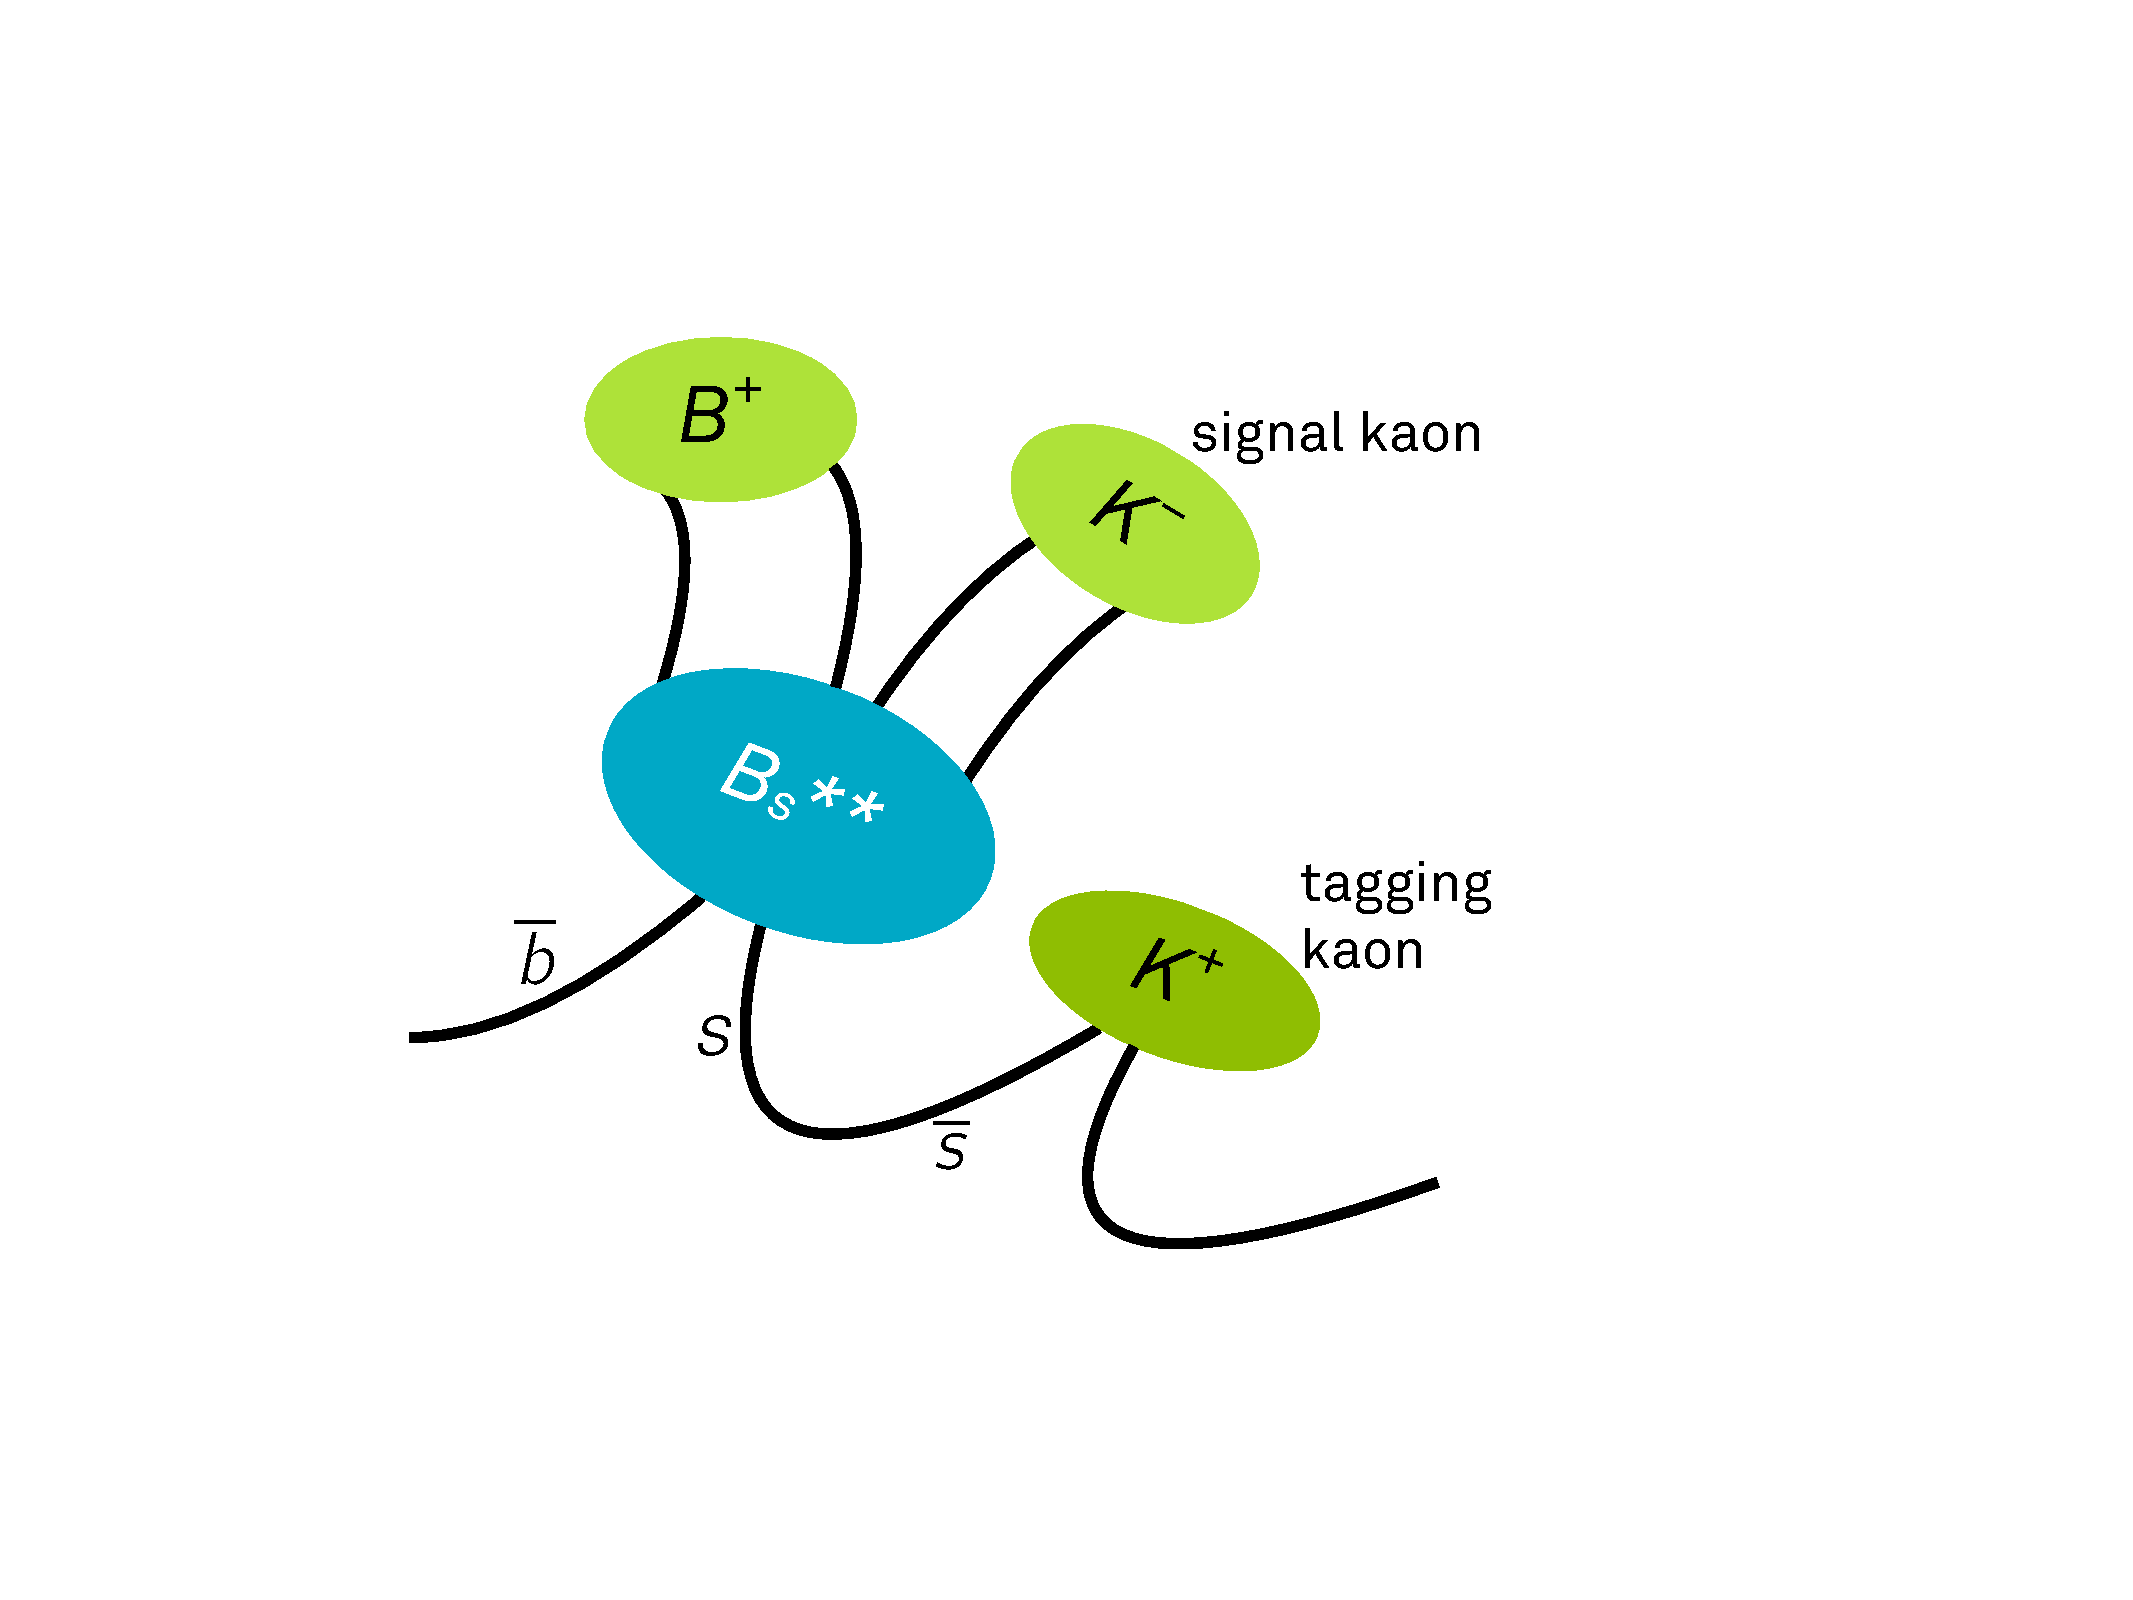
\includegraphics[width=0.608\textwidth]{figures/Bscalib.pdf}
\end{center}
\vspace{-1.7em}
\begin{itemize}
\setlength\itemsep{0.01em}
%\item further excited \Bs states are considered:
%\begin{itemize}
%\setlength\itemsep{0.01em}
%\setlength{\itemindent}{-.11in}
%\item[${\color{tu_gruen}-}$] $B_{s1}/B_{s2}^*\to B^{*+}K$
%\item[${\color{tu_gruen}-}$] add just few statistics
%\item[${\color{tu_gruen}-}$] missing \g from $B_{s1,2}^*\to\B\g$ is challenging
%\item[${\color{white}-}$] changes kinematic distributions of $B_{s1,2}$
%\end{itemize}
%\end{itemize}
%\begin{center}
%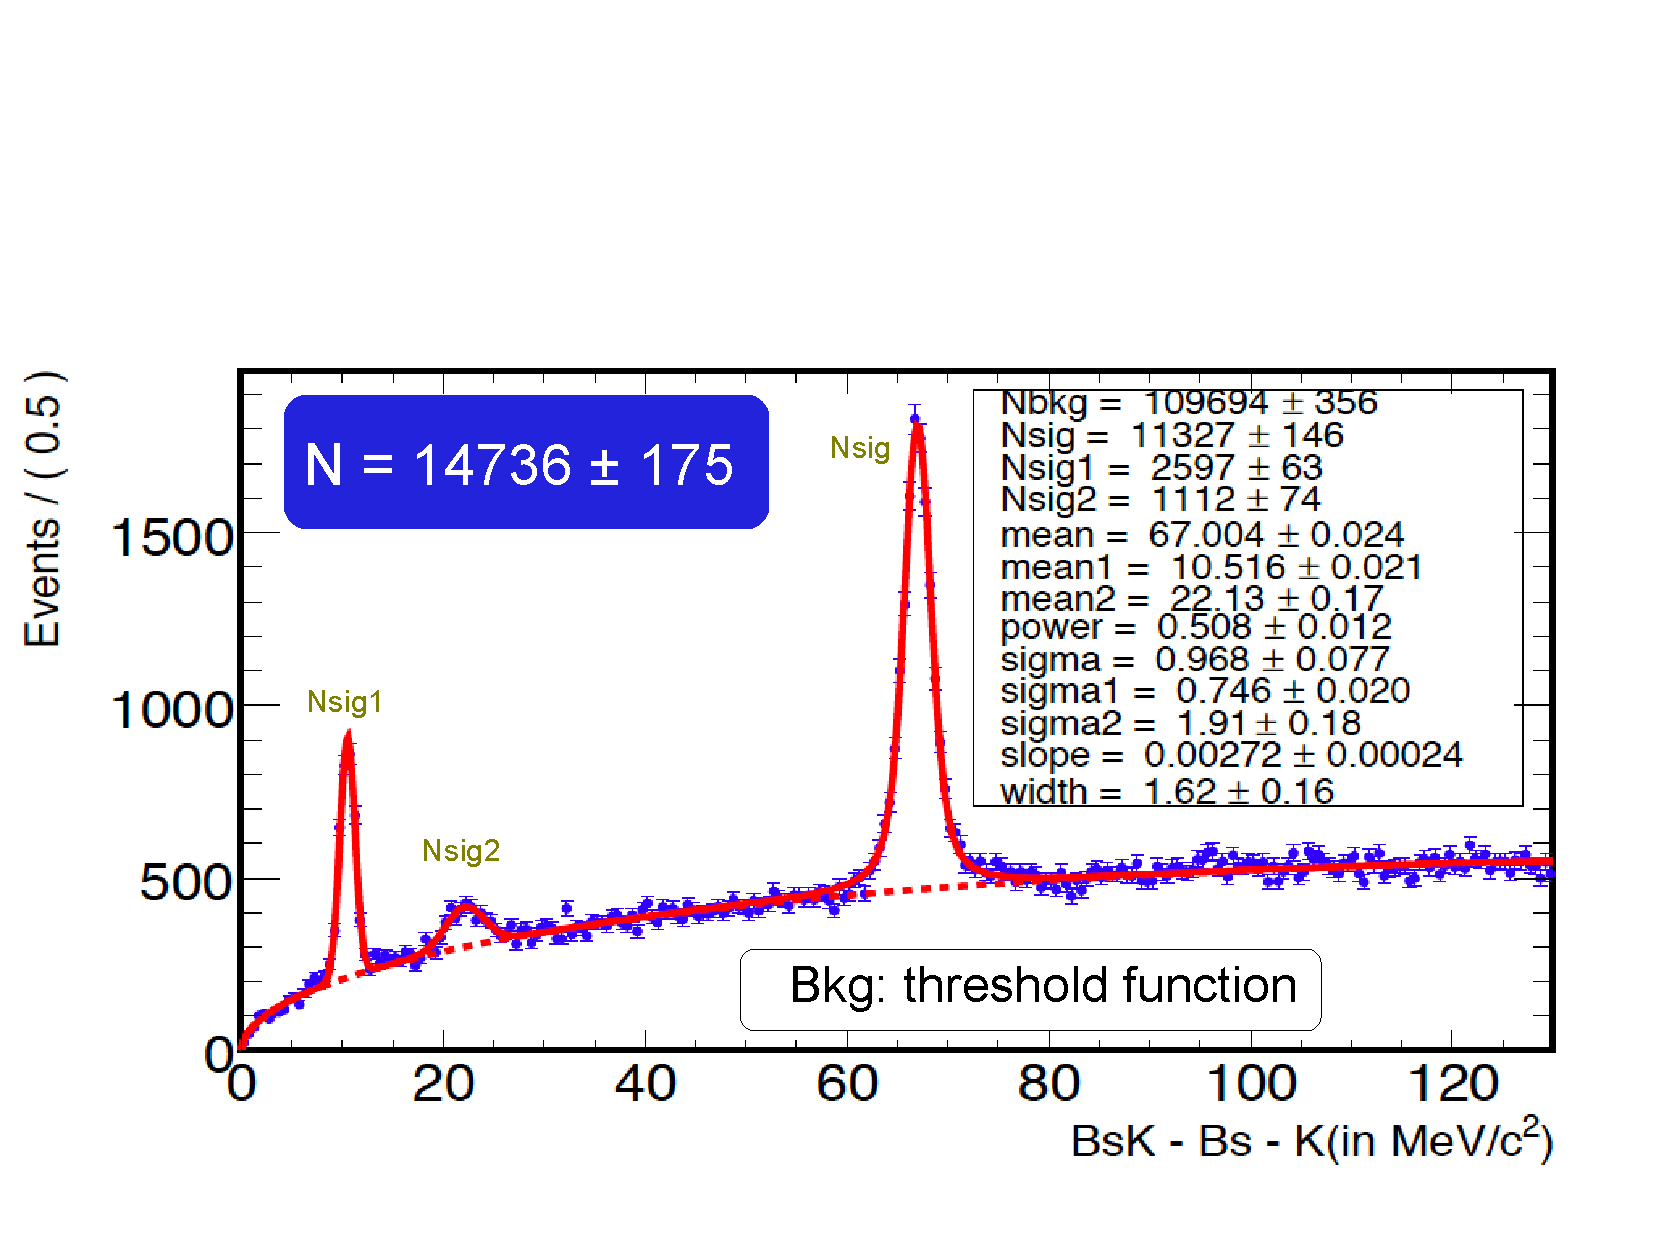
\includegraphics[width=\textwidth]{figures/BsdoublestarMass.pdf}%dürfen wir diesen Plot so zeigen?? -> ist aus dem PPTS Vortrag
%\end{center}
%\begin{itemize}
\item true independent crosscheck for \BsToDspi
\item results in agreement with \BsToDspi channel
%\item statistical uncertainties still limited
%\begin{equation*}
%\Delta p_0=0.002\pm0.011\hspace{0.5cm} \Delta p_1=-0.22\pm0.017 %ich weiß nicht ob wir diese Zahlen zeigen dürfen, vermute eher nicht
%\end{equation*}
%\vspace{-1.7em}
%\item analysis note in preparation
\end{itemize}

\vspace{0.1em}

\textbf{SS pion calibration}
\vspace{-0.1em}
\begin{itemize}
\setlength\itemsep{0.01em}
\item calibration performed with \BdToJPsiKst
\item full evaluation of systematic uncertainties 
%\begin{equation*}
%\begin{aligned}
%  p_0^{\text{SS\pion}}        &= \phantom{-}0.4232  \,\pm\, 0.0029           \text{\,(stat)} \,\pm\, 0.0020           \text{\,(syst)} \\ 
%  p_1^{\text{SS\pion}}        &= \phantom{-}1.011\phantom{0}   \,\pm\, 0.064\phantom{0} \text{\,(stat)} \,\pm\, 0.009\phantom{0} \text{\,(syst)} \\ 
%  \Delta p_0^{\text{SS\pion}} &= -0.0026 \,\pm\, 0.0043           \text{\,(stat)} \,\pm\, 0.0024           \text{\,(syst)}  \\
%  \Delta p_1^{\text{SS\pion}} &= -0.171\phantom{0}   \,\pm\, 0.096\phantom{0} \text{\,(stat)} \,\pm\, 0.029\phantom{0} \text{\,(syst)} \\
%  \langle\eta^{\text{SS\pion}}\rangle        &= \phantom{-}0.425\phantom{0} 
%\end{aligned}
%\end{equation*}
\item used for the first time in the measurements of
\begin{itemize}
\setlength{\itemindent}{-.11in}
\item[${\color{tu_gruen}-}$] $\sin(2\beta)$ with $\Bd \rightarrow \jpsi K_S^0$
\setlength{\itemindent}{.05in}
\item[${\color{tu_gruen}\Rightarrow}$] precision comparable to $B$-factories
\item[${\color{tu_gruen}\Rightarrow}$] $\varepsilon_{\text{eff}}^{\text{SS}\pion} = 0.38\,\%$
\setlength{\itemindent}{-.11in}
\item[${\color{tu_gruen}-}$] $\sin(2\beta_{\text{eff}})$ with $\Bd \rightarrow \jpsi \pi^+ \pi^-$
\setlength{\itemindent}{.05in}
\item[${\color{tu_gruen}\Rightarrow}$] $\varepsilon_{\text{eff}}^{\text{SS}\pion} = 0.54\,\%$
\end{itemize}


%\begin{equation*}
%\begin{aligned}
%&\Bd \rightarrow \jpsi K_S^0: &\varepsilon_{\text{eff}}^{\text{SS}\pion} &= 0.54\,\% \\
%&\Bd \rightarrow \jpsi \pi^+ \pi^-: &\varepsilon_{\text{eff}}^{\text{SS}\pion} &= 0.376\,\% 
%\end{aligned}
%\end{equation*}

\end{itemize}
\end{minipage}
\vspace{0.1em}
\hfill
\begin{minipage}{0.474\boxwidth}
\textbf{OS and SS Kaon tagging using neural nets (NN)}
\vspace{-0.1em}
\begin{itemize}
\item basic idea: use two NN
\begin{itemize}
\setlength\itemsep{0.01em}
\setlength{\itemindent}{-.11in}
\item[${\color{tu_gruen}-}$] first NN distinguishes between:
\begin{enumerate}
\item fragmentation tracks\\
${\color{tu_gruen}\Rightarrow}$ signal for SS kaon nnet
\item OS $b$ hadron tracks\\
${\color{tu_gruen}\Rightarrow}$ signal for OS kaon nnet
\item underlying event tracks 
\end{enumerate}
\end{itemize}
\vspace{-1.7em}
\begin{center}
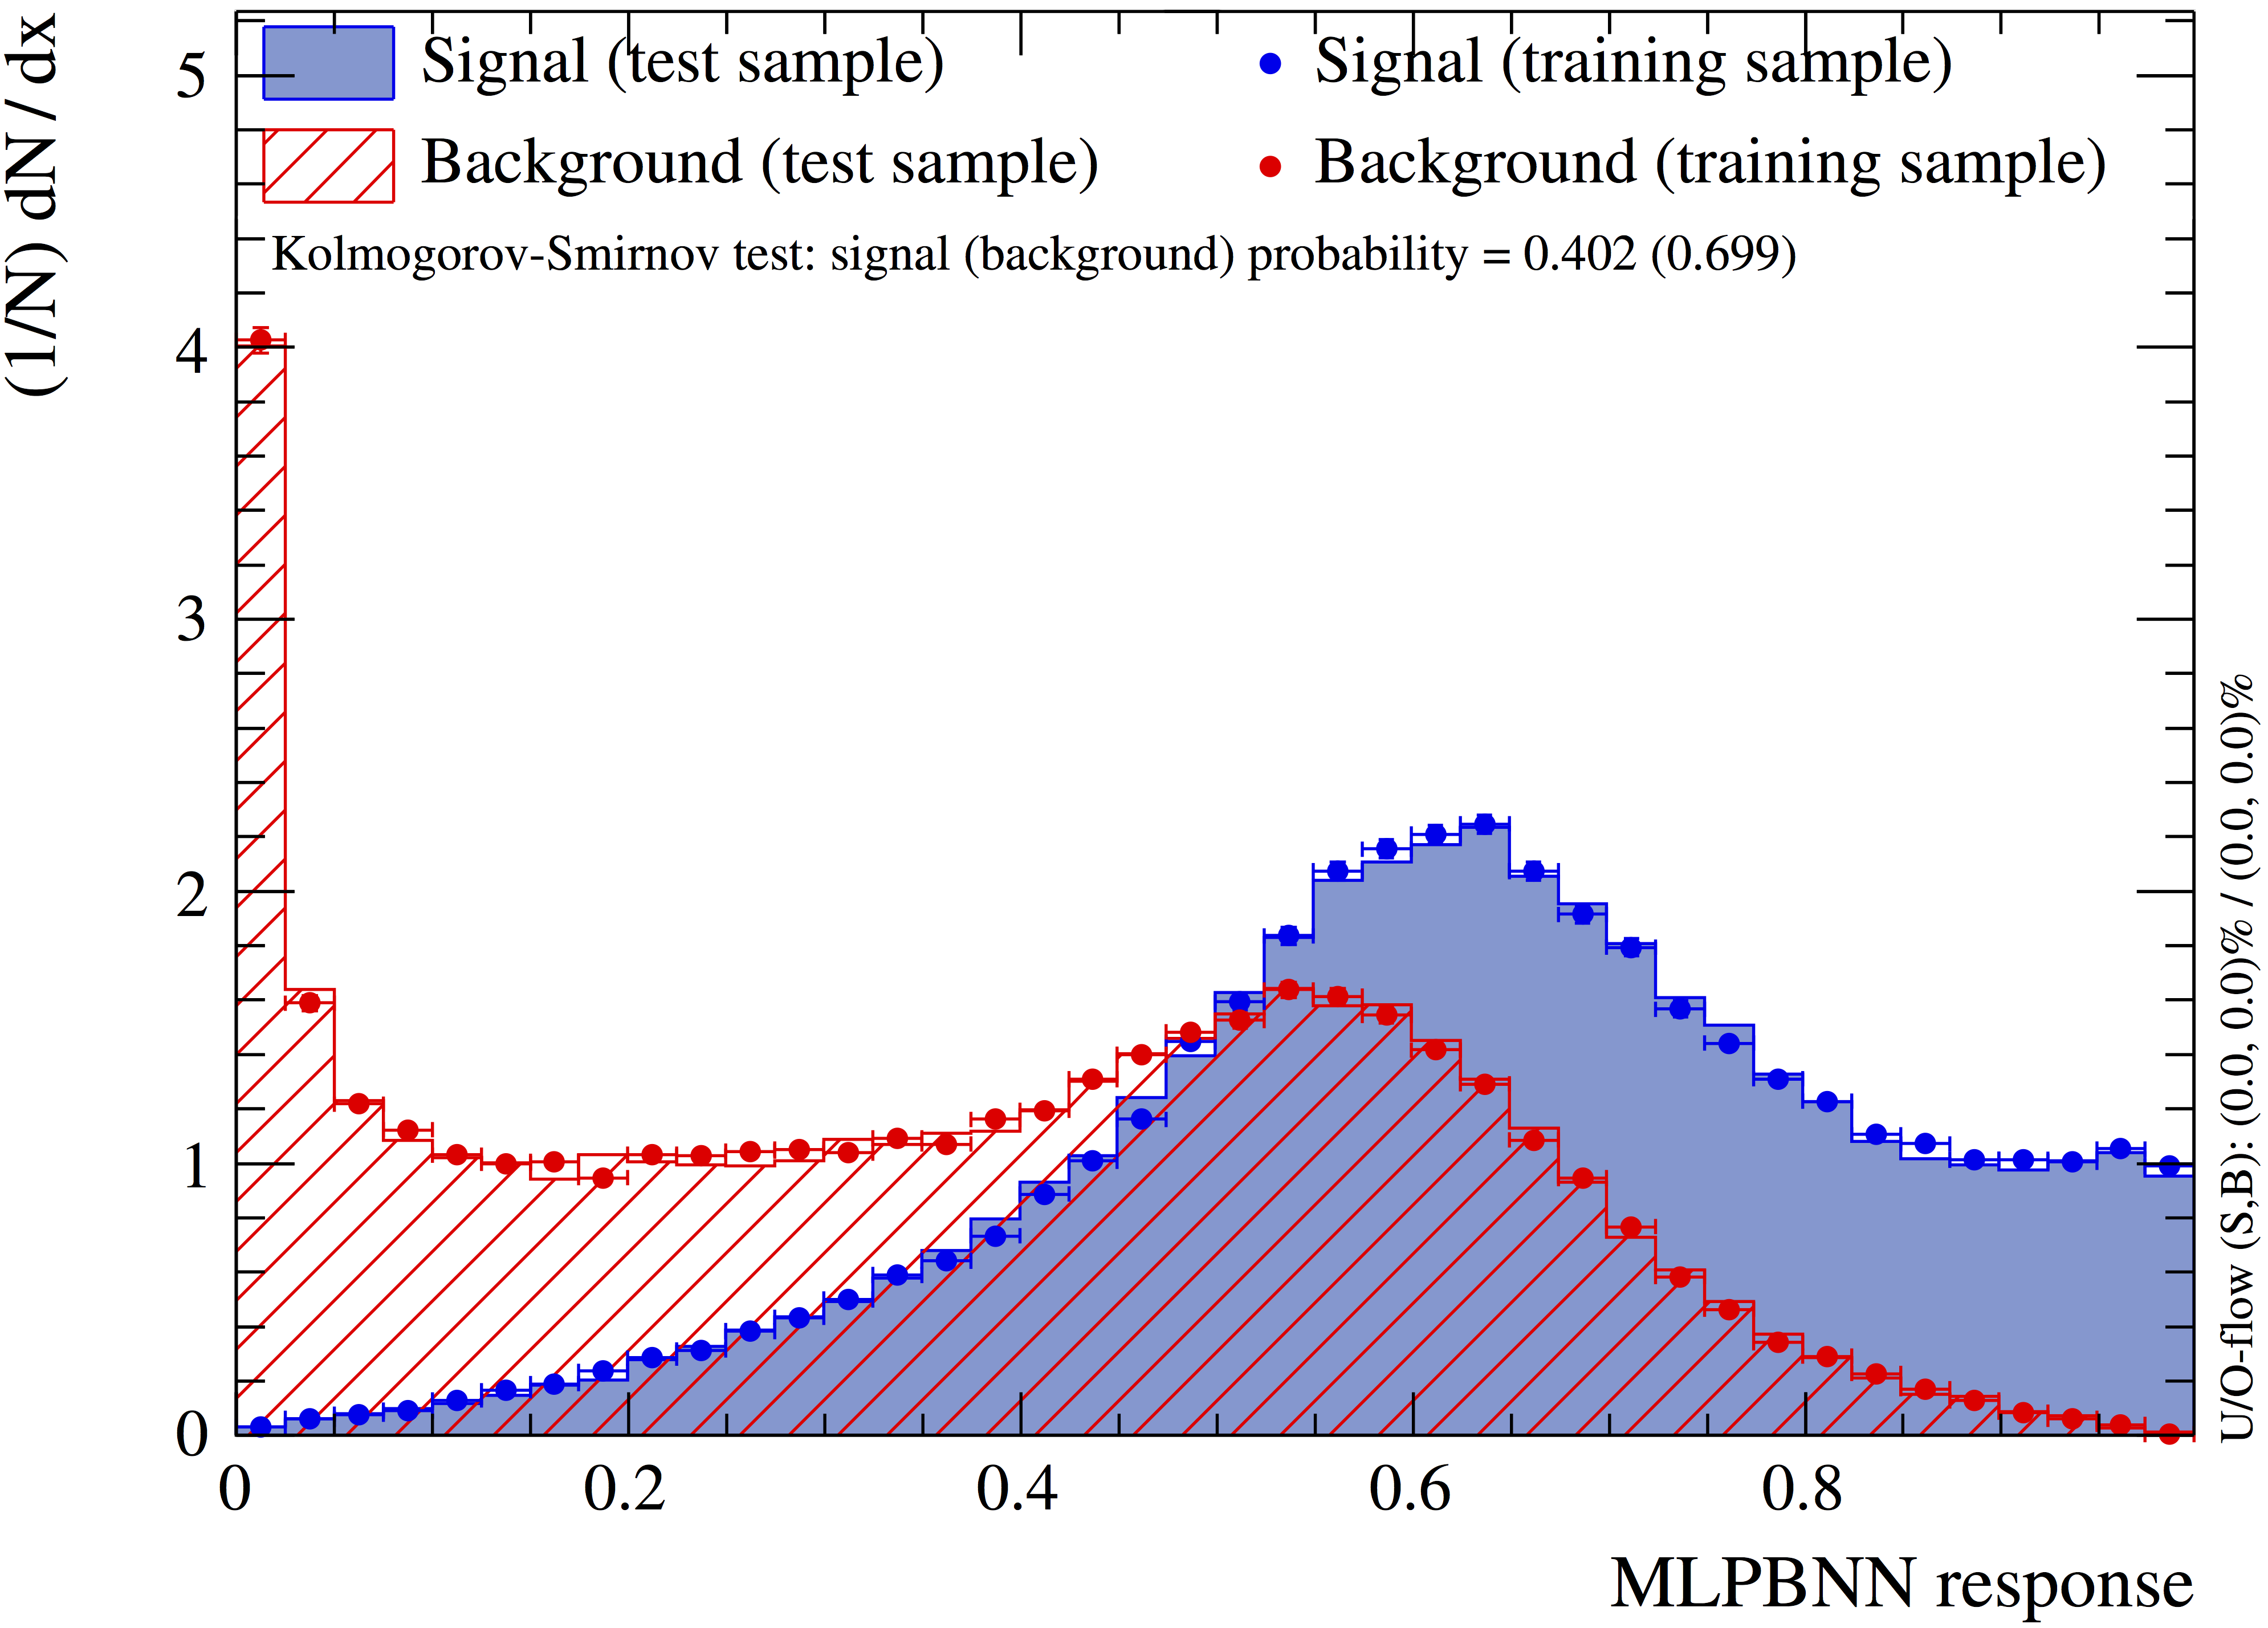
\includegraphics[width=0.802\textwidth]{figures/sskaonNnetfirstNN3.png}
\end{center}
\vspace{-2.5em}
\setlength\itemsep{0.01em}
\setlength{\itemindent}{-.11in}
\begin{itemize}
\setlength{\itemindent}{-.11in}
\item[${\color{tu_gruen}-}$] second NN:
\begin{itemize}
\item[${\color{tu_gruen}\circ}$] receives up to 3 candidates 
\item[${\color{tu_gruen}\circ}$] assigns final tag and mistag
\end{itemize}
\end{itemize}
\end{itemize}
\begin{itemize}
\setlength\itemsep{0.01em}
%\item both taggers have a high efficiency
\item SS kaon nnet tagger is a great success, compared \newline to the previous cut-based SS kaon it gives  
\begin{itemize}
\setlength{\itemindent}{-.11in}
\vspace{-0.5em}
\item[${\color{tu_gruen}-}$] \BsToDspi: $50\,\%$ relative improvement in $\varepsilon_{\text{eff}}$
\item[${\color{tu_gruen}-}$] \BsToJPsiPhi: $41\,\%$ relative improvement in $\varepsilon_{\text{eff}}$
\end{itemize}
%\item combined paper for both taggers in preparation
%\item SS kaon nnet:
%\begin{itemize}
%\setlength\itemsep{0.01em}
%\setlength{\itemindent}{-.11in}
%\item[${\color{tu_gruen}-}$] high mistag tagger: mean mistag O(43\%)
%\item[${\color{tu_gruen}-}$] compensating this with high statistics
%\item[${\color{tu_gruen}-}$] Improves tagging power by 40 \%
%\setlength\itemsep{0.01em}
%\setlength{\itemindent}{-.11in}
%\item[${\color{tu_gruen}-}$] improve selection of fragmentation tracks with neural network (trained on $\Bs\to\Ds\pi$)
%\item[${\color{tu_gruen}-}$] a second neural network, which computes the mistag and the tagging decision combines up to 3 multiple candidates
%\end{itemize}
%\begin{center}
%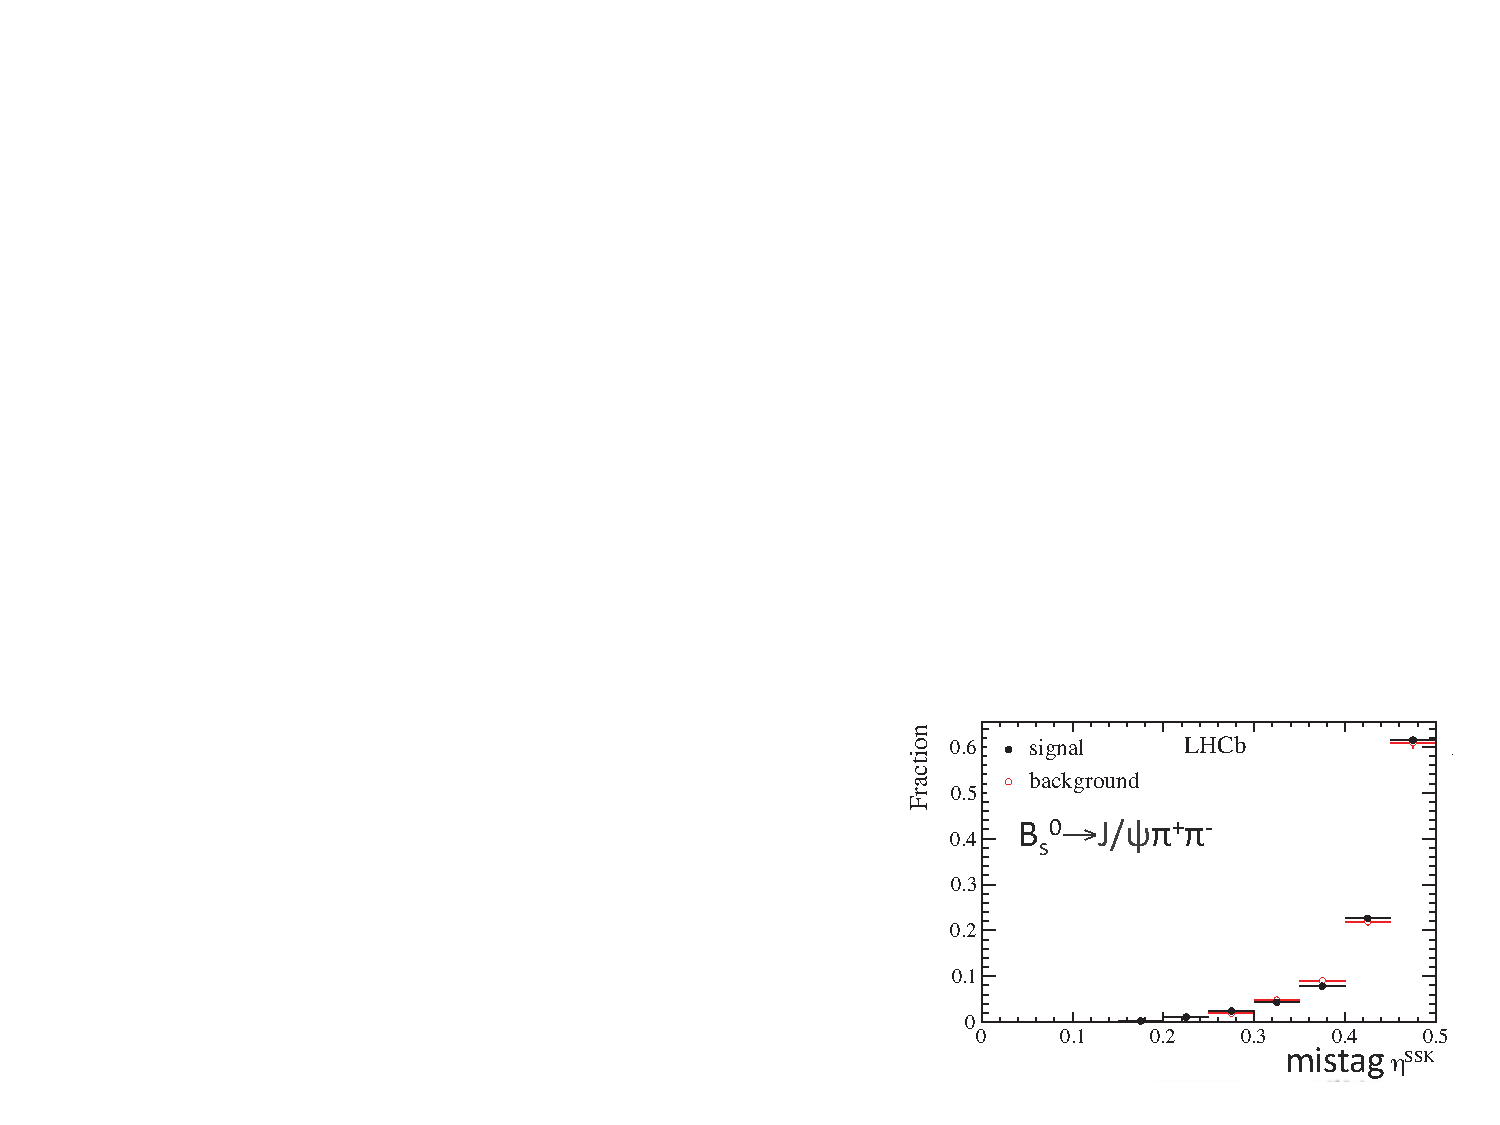
\includegraphics[width=0.8\textwidth]{figures/mistag_sskaonNN.pdf}
%\end{center}
\end{itemize}
\vspace{-0.1em}
\textbf{OS charm tagger}
\vspace{-0.15em}
\begin{itemize}
\setlength\itemsep{0.01em}
\item reconstruct $D^0$/$D^\pm$/$D^*$ decays related to OS $b$ decay
\item one boosted decision tree (BDT) for each mode
\item clean measure of \B meson flavour (low mistag) 
\item adds about $0.37\,\%$ to $\epsilon_{\text{eff}}$
%\item analysis note in preparation
\end{itemize}
\vspace{0.2em}
\textbf{SS pion BDT and SS proton}
\vspace{-0.1em}
\begin{itemize}
\setlength\itemsep{0.01em}
\item promising new taggers based on BDT's
\item development ongoing
\end{itemize}
\vspace{-0.75em}
\end{minipage}
}




%combine NNet Tagger chapters
%% !TEX root = poster.tex
%\headerbox{Outlook}{name=out,column=2,row=2,below=run1,above=refs}{
\headerbox{\textbf{Outlook on Run II}}{name=out,column=1,row=2,span=2,below=devs}{
\begin{minipage}{0.474\boxwidth}
\textbf{Effects of new conditions}
\vspace{-0.1em}
\begin{itemize}
\setlength\itemsep{0.01em}
\item \lhc will run at $\sqrt{s}=$13\,TeV 
\setlength{\itemindent}{.14in}
\item[${\color{red}\downarrow}$] higher track multiplicity (degrades OS/SS taggers)
\item[${\color{green}\uparrow}$] higher $B$ momentum (improves SS taggers)
\setlength{\itemindent}{.in}
\item luminosity leveling at \lhcb
\setlength{\itemindent}{.14in}
\item[${\color{green}\uparrow}$] lower PV multiplicity (improves OS/SS taggers)
\setlength{\itemindent}{0.in}
%\item[${\color{tu_gruen}\uparrow}$] effects should balance in FT performance
%\item[${\color{tu_gruen}\Rightarrow}$] first checks on simulations are encouraging
\end{itemize}
\vspace{-0.47em}
\end{minipage}
\hfill
\begin{minipage}{0.474\boxwidth}
\vspace{-0.70em}
\textbf{Preparations}
\vspace{-0.1em}
\begin{itemize}
\setlength\itemsep{0.01em}
\item taggers are optimised for Run I
\setlength{\itemindent}{.14in}
\item[${\color{tu_gruen}\Rightarrow}$] need to optimise tagging candidates’ selections
\item[${\color{tu_gruen}\Rightarrow}$] retrain with simulations of the 2015 conditions... 
\item[${\color{tu_gruen}\Rightarrow}$] ...and check performances with first data
\setlength{\itemindent}{0.in}
\item recalibrate and reoptimise all taggers
\end{itemize}
%\vspace{0.3em}
\end{minipage}

}
% !TEX root = poster.tex
\headerbox{\textbf{References}}{name=refs,column=1,row=3,span=2,above=bottom}{
%\hspace{0.18em}
\begin{minipage}{0.474\boxwidth}
%\vspace{-0.6em}
\begin{compactitem}
{\tiny\item[{[1]}] LHCb Collaboration, R. Aaij et. al., {\it Opposite-side flavour tagging of \B mesons at the \lhcb experiment, Eur.Phys.J.} C72 (2012) 2022}
\end{compactitem}
\begin{compactitem}
{\tiny\item[{[2]}] LHCb Collaboration, R. Aaij et. al., {\it Optimization and calibration of the same-side kaon \mbox{tagging} algorithm using hadronic \Bs decays in 2011 data,} \lhcb-CONF-2012-033}
\end{compactitem}
\begin{compactitem}
{\tiny\item[{[3]}] LHCb Collaboration, R. Aaij et. al., {\it Measurement of \CP violation and the \Bs meson decay width difference with  \BsToJPsiKK and \BsToJPsipipi decays, } Phys.Rev. D87 (2013) 112010}
\end{compactitem}
\begin{compactitem}
{\tiny\item[{[4]}] LHCb Collaboration, R. Aaij et. al., {\it Precision measurement of \CP violation in \BsToJPsiKK decays, } Phys.Rev.Lett. 114 (2015) 4 041801}
\end{compactitem}
\begin{compactitem}
{\tiny\item[{[5]}] LHCb Collaboration, R. Aaij et. al., {\it Measurement of the CP-violating phase $\phi_s$ in \BsToJPsipipi decays, } Phys.Lett. B713 (2012) 378-386}
\end{compactitem}
\begin{compactitem}
{\tiny\item[{[6]}] LHCb Collaboration, R. Aaij et. al., {\it Measurement of the CP-violating phase $\phi_s$ in \BsToJPsipipi decays, } Phys.Lett. B736 (2014) 186}
\end{compactitem}
\begin{compactitem}
{\tiny\item[{[7]}] LHCb Collaboration, R. Aaij et. al., {\it Measurement of the \CP-violating phase $\phi_s$ in \BsToDsDs decays, } Phys.Rev.Lett. 113 (2014) 211801}
\end{compactitem}
\vspace{0.10em}
\end{minipage}
\hfill
\begin{minipage}{0.474\boxwidth}
\begin{compactitem}
{\tiny\item[{[8]}] LHCb Collaboration, R. Aaij et. al., {\it Measurement of \CP asymmetry in \BsToDsK decays, } JHEP 1411 (2014) 060}
\end{compactitem}
\begin{compactitem}
{\tiny\item[{[9]}] LHCb Collaboration, R. Aaij et. al., {\it Measurement of the time-dependent \CP asymmetry in \BdToJPsiKS decays, } Phys.Lett. B721 (2013) 24-31}
\end{compactitem}
\begin{compactitem}
{\tiny\item[{[10]}] LHCb Collaboration, R. Aaij et. al., {\it Measurement of \CP violation in \BdToJPsiKS decays, } Phys.Rev.Lett. 115 (2015) 031601}
\end{compactitem}
\begin{compactitem}
{\tiny\item[{[11]}] LHCb Collaboration, R. Aaij et. al., {\it Measurement of the time-dependent \CP asymmetries in \BsToJPsiKS, } JHEP 1506 (2015) 131}
\end{compactitem}
\begin{compactitem}
{\tiny\item[{[12]}] LHCb Collaboration, R. Aaij et. al., {\it \B flavor tagging using reconstructed charm decays at the LHCb experiment, } LHCb-PAPER-2015.027}
\end{compactitem}
\begin{compactitem}
{\tiny\item[{[13]}] G. A. Krocker, {\it Development and calibration of a same side kaon tagging algorithm and measurement of the $\Bs-\Bsb$ oscillation frequency \dms at the LHCb experiment, } PhD thesis, Heidelberg U., Sep, 2013, CERN-THESIS-2013-213}
\end{compactitem}
\vspace{0.10em}
\end{minipage}

}









\end{poster}%
\end{document}